\documentclass[a4paper]{article}
\usepackage{fullpage}
\usepackage{graphicx}
\usepackage{xcolor}

\IfFileExists{.git/gitHeadInfo.gin}{
    \usepackage[pcount,grumpy,mark,markifdirty]{gitinfo2}
}{%
    \usepackage[local,pcount,grumpy,mark,markifdirty]{gitinfo2}
}




%%%%%%%%%%%%%%%%%%%%%%%%%%%%%%%%%%%%%%%%%%%%%%%%%%%%%%%%%%%%%%%%%%%%%%%%%%%%%%%%%%%%%%%%%%%%%%%%%%%%%%%%%%%%%%%%%%%%%%%%
% Load packages
\usepackage{bbm}
\usepackage{amsmath,amsthm,amsfonts,amssymb}
\usepackage{stmaryrd}
\usepackage{graphicx}
\usepackage{subfigure}
\usepackage{multicol,multirow}
\usepackage{paralist}
\usepackage{textcomp}
\usepackage[ruled]{algorithm2e}
\usepackage[nopatch=footnote]{microtype}
\usepackage{indentfirst}
\usepackage{lmodern}
\usepackage{stmaryrd}
\usepackage{fixmath}
\usepackage{csvsimple}
\usepackage{numprint}
\usepackage{soul}
\usepackage{booktabs}
\SetSymbolFont{stmry}{bold}{U}{stmry}{m}{n}
\usepackage{textgreek}
\usepackage{siunitx}
\usepackage{listofitems} % for \readlist to create arrays
\usepackage{pgfplotstable} % <-- required in preamble
\usepackage{import}
\usepackage{currfile}

\usepackage{csquotes}
\usepackage[backend=biber, style=alphabetic]{biblatex}
\addbibresource{biblio.bib}

\usepackage{pgfplots}
\usepackage{pgfplotstable}
\pgfplotsset{compat=newest}

\usepgfplotslibrary{fillbetween}
\usetikzlibrary{positioning,shapes,shadows,arrows,angles,quotes,decorations.markings}
\usetikzlibrary{mindmap, backgrounds}
\usepgfplotslibrary{groupplots}
\usetikzlibrary{pgfplots.colormaps}


\tikzstyle{abstract}=[rectangle, draw=black, fill=blue!30, drop shadow,text centered, anchor=north, text=black]

\definecolor{colorFeel3}{RGB}{28, 142, 186}
\definecolor{colorFeel2}{RGB}{226, 19, 19}
\definecolor{colorOoi}{RGB}{34, 120, 15}
\definecolor{colorScott}{RGB}{244, 102, 27}
\definecolor{colorLi}{RGB}{108, 2, 119}

\definecolor{colorA}{RGB}{49,140,231}
\definecolor{colorB}{RGB}{238,16,16}

\definecolor{crimson2143940}{RGB}{214,39,40}
\definecolor{darkgray176}{RGB}{176,176,176}
\definecolor{darkorange25512714}{RGB}{255,127,14}
\definecolor{forestgreen4416044}{RGB}{44,160,44}
\definecolor{lightgray204}{RGB}{204,204,204}
\definecolor{steelblue31119180}{RGB}{31,119,180}
\definecolor{mediumpurple148103189}{RGB}{148,103,189}

\newcommand{\logLogSlopeTriangle}[5]
{
    % #1. Relative offset in x direction.
    % #2. Width in x direction, so xA-xB.
    % #3. Relative offset in y direction.
    % #4. Slope d(y)/d(log10(x)).
    % #5. Plot options.

    \pgfplotsextra
    {
        \pgfkeysgetvalue{/pgfplots/xmin}{\xmin}
        \pgfkeysgetvalue{/pgfplots/xmax}{\xmax}
        \pgfkeysgetvalue{/pgfplots/ymin}{\ymin}
        \pgfkeysgetvalue{/pgfplots/ymax}{\ymax}

        \pgfmathsetmacro{\xArel}{#1}
        \pgfmathsetmacro{\yArel}{#3}
        \pgfmathsetmacro{\xBrel}{#1-#2}
        \pgfmathsetmacro{\yBrel}{\yArel}
        \pgfmathsetmacro{\xCrel}{\xArel}

        \pgfmathsetmacro{\lnxB}{\xmin*(1-(#1-#2))+\xmax*(#1-#2)} % in [xmin,xmax].
        \pgfmathsetmacro{\lnxA}{\xmin*(1-#1)+\xmax*#1} % in [xmin,xmax].
        \pgfmathsetmacro{\lnyA}{\ymin*(1-#3)+\ymax*#3} % in [ymin,ymax].
        \pgfmathsetmacro{\lnyC}{\lnyA+#4*(\lnxA-\lnxB)}
        \pgfmathsetmacro{\yCrel}{(\lnyC-\ymin)/(\ymax-\ymin)} % THE IMPROVED EXPRESSION WITHOUT 'DIMENSION TOO LARGE' ERROR.

        \coordinate (A) at (rel axis cs:\xArel,\yArel);
        \coordinate (B) at (rel axis cs:\xBrel,\yBrel);
        \coordinate (C) at (rel axis cs:\xCrel,\yCrel);

        \draw[#5]   (A) -- % node[pos=0.5,anchor=north] {1}
                    (B) --
                    (C) -- node[pos=0.5,anchor=west] {\pgfmathprintnumber[precision=2]{#4}}
                    cycle;
    }
}


%%% Math macros
\newcommand{\vct}[1]{\mathbold{#1}}
\newcommand{\mat}[1]{\mathbold{#1}}
\DeclareMathOperator*{\argmax}{arg\,max}

\newcommand{\E}{\mathbb{E}}
\newcommand{\Em}{\mathcal{E}}
\newcommand{\Dmu}{D^{\mu}}
\newcommand{\N}{\mathcal{N}}
\newcommand{\n}{\vct{n}}
\renewcommand{\P}{\mathbb{P}}
\newcommand{\R}{\mathbb{R}}

\newcommand{\fem}{\mathrm{fem}}
\newcommand{\fpp}{Feel++}
\newcommand{\lb}{\mathrm{lb}}
\newcommand{\rbm}{\mathrm{rbm}}
\newcommand{\test}{\text{test}}
\newcommand{\tol}{\text{tol}}
\newcommand{\train}{\text{train}}
\newcommand{\ub}{\mathrm{ub}}
\newcommand{\var}{\mathrm{var}}
\newcommand{\x}{\vct{x}}

\newcommand{\logN}{\log\text{-}\mathcal{N}}
\newcommand{\unif}{\mathcal{U}}

\newcommand{\norm}[2]{\left\Vert#1\right\Vert_{#2}}
\newcommand{\scal}[3]{\left<#1,#2\right>_{#3}}
\newcommand{\prm}[1]{\textcolor{blue}{#1}}

%%% Theorems
\theoremstyle{plain}
\newtheorem{thm}{Theorem}[section]
\newtheorem{prop}[thm]{Proposition}
\newtheorem{coro}[thm]{Corollary}
\newtheorem{lem}[thm]{Lemma}

\theoremstyle{definition}
\newtheorem{defi}[thm]{Definition}
\newtheorem{ex}[thm]{Example}
\newtheorem{nota}[thm]{Notation}
\newtheorem{rem}[thm]{Remark}
\usepackage{hyperref}
\usepackage[noabbrev]{cleveref}
\usepackage{xurl}

\makeatletter
\title{Model order reduction and sensitivity analysis for complex heat transfer simulations inside the human eyeball}
\author{%
    \texorpdfstring{
        Thomas Saigre\textsuperscript{1}\textsuperscript{$\dagger$}, Christophe Prud'homme\textsuperscript{1}, Marcela Szopos\textsuperscript{2}\\
        \small\textsuperscript{1}Institut de Recherche Mathématique Avancée, UMR 7501 Université de Strasbourg et CNRS\\
        \small\textsuperscript{2}Université Paris Cité, CNRS, MAP5, F-75006 Paris, France\\
        \small\textsuperscript{$\dagger$}Corresponding author contact: \texttt{saigre@math.unistra.fr}
    }{Thomas Saigre, Christophe Prud'homme, Marcela Szopos}
}
\date{\gitReln\  \gitAuthorDate\ (\gitAbbrevHash)}

% Define custom color
\definecolor{CustomBlue}{rgb}{0.25, 0.41, 0.88} % RoyalBlue
% Set up hyperref with the custom citecolor
\hypersetup{
    pdftitle={\@title},
    pdfauthor={\@author},
    % pdfsubject={\@subject},
    pdfkeywords={LaTeX, GitHub Actions, Zotero, Overleaf},
    bookmarksnumbered,bookmarksopen,linktocpage,
    colorlinks=true,
    citecolor=CustomBlue,
    linkcolor=CustomBlue,
    urlcolor=blue
}
\makeatother
\renewcommand{\d}{\,\mathrm{d}}


\begin{document}

\maketitle

\begin{abstract}
    Heat transfer in the human eyeball, a complex organ, is significantly influenced by various pathophysiological and external parameters.
    Particularly, heat transfer critically affects fluid behavior within the eye and ocular drug delivery processes.
    Overcoming the challenges of experimental analysis, this study introduces a comprehensive three-dimensional mathematical and computational model to simulate the heat transfer in a realistic geometry.
    Our work includes an extensive sensitivity analysis to address uncertainties and delineate the impact of different variables on heat distribution in ocular tissues.
    To manage the model's complexity, we employed a very fast model reduction technique with certified sharp error bounds, ensuring computational efficiency without compromising accuracy.
    Our results demonstrate remarkable consistency with experimental observations and align closely with existing numerical findings in the literature.
    Crucially, our findings underscore the significant role of blood flow and environmental conditions, particularly in the eye's internal tissues.
    Clinically, this model offers a promising tool for examining the temperature-related effects of various therapeutic interventions on the eye.
    Such insights are invaluable for optimizing treatment strategies in ophthalmology.
\end{abstract}

\tableofcontents



\vspace{\baselineskip}

\noindent
\textbf{Keywords :} mathematical and computational ophthalmology, heat transfer, validation, finite element method, real-time model order reduction, uncertainty quantification, sensitivity analysis, Sobol index analysis.

% 1. Introduction
%!TeX root=../article.heat-fom-rom-sa.ijnmbe24.tex
\section{Introduction}
\label{sec:intro}

The development of new technologies allows us to simulate more and more complex models in order to apprehend the world we live in.
In this study, we will focus on a specific model: heat transfer inside the human eyeball.
The temperature of the eyeball may have an impact on the distribution of drugs in the eye, partly due to the aging of the tissues \cite{BHANDARI2020286}.
Hyperthermia is one of the most common treatments for eye tumors~\cite{li2010}, and understanding the mechanism of heat transfer could enhance the efficacy of ophthalmic treatments, such as laser therapy of the retina~\cite{Masters2004}.

Heat transfer is also a key factor in the study of the effects of electromagnetic radiation on the eye, as pointed out in \cite{Hirata2007,doi:10.1142/S0219519409002936}.
The model, originally introduced in \cite{Scott_1988} to examine temperature rises induced by exposure to infrared radiation,
has been expanded upon in subsequent studies \cite{NG2006268, NG2007829, OOI2008252, li2010} using diverse methods for computing heat transfer.

While invasive studies on animals have been conducted \cite{Purslow2005-ky}, non-invasive measurements on human subjects are scarce, complex to perform, and may yield inaccurate results \cite{ROSENBLUTH1977325}.
Most studies focus on temperature measurements at the eye's surface \cite{MAPSTONE1968237, Efron1989OcularST} but report significant differences and identify several sources of uncertainty.
Alternatively, numerical simulations can provide complementary information.
However, in order to guarantee the reliability of such results, a rigorous validation step is required.

The present contribution aims to contribute to these developments, by means of a mathematical and computational modeling approach, combined with a sensitivity analysis study performed thanks to a model reduction technique.
The comparison with data available in the literature, obtained either by measurement on healthy subjects~\cite{Efron1989OcularST} or by other simulations \cite{NG2006268, NG2007829, li2010} will ensure the validity of the approach.

In this model, numerous parameters, both biomechanical and geometrical, are involved.
The present study concentrates on biomechanical parameters, in a large range that include potential extremal conditions.
The variation of these parameters can have a significant impact on the results.
To quantify their impact, we set up a framework to perform a forward uncertainty quantification study, complemented by a sensitivity analysis.
Deterministic sensitivity analysis has already been performed in \cite{Scott_1988, NG2006268, NG2007829, li2010}, using various numerical methods.
In this work, we reproduce and extend these results, to incorporate the effect of blood flow, as suggested for instance in \cite{Scott_1988}.
We also run a global sensitivity analysis, that accounts for stochastic effects, and discriminate among different factors by means of Sobol's indices \cite{Sobol1993SensitivityEF}.
The combination of deterministic and stochastic methods is an effective practice in the field of uncertainty quantification, and has been successfully used in recent various applications, such as \cite{DODIG201448} where the impact of uncertainties on the distribution of the electromagnetic field in the ocular tissue is studied;
or more generally in the human head \cite{SUSNJARA20221,9522096}.
To the best of our knowledge, this is the first time that such a study is performed in the context of bioheat transport in the tissues of the human eyeball.

While Sobol's indices are effective in measuring parameter impact and interactions, the complexity and the significant computational time of our model are very challenging.
To overcome this, we adopt the certified reduced basis method \cite{10.1115/1.1448332, Quarteroni2016} to obtain a reduced model, maintaining its 3D nature while significantly reducing computational demands.
This method aligns with the paradigm observed in patient-specific mathematical models applied to biomedical problems,
ensuring a comprehensive approach involving data integration, model derivation, numerical solving, validation, and uncertainty quantification, as seen in mature research fields like cardiovascular simulations or cerebral hemodynamics.
In ophthalmology, a similar paradigm is imperative due to the richness and heterogeneity of available data, requiring innovative approaches for diagnosis and monitoring.

More generally, the present work aims to contribute to the project Eye2Brain \cite{eye2brain},
that has the ambitious objective to connect the cerebral and ocular environments and contribute in the long term to a better understanding of neurodegenerative diseases~\cite{Guidoboni2020-vr}.
In this context, a model accounting for the combined effects of ocular blood flow and different ocular tissues was proposed in \cite{https://doi.org/10.1002/cnm.3791}0
To incorporate inherent uncertainties and variability, an uncertainty propagation and sensitivity analysis on the component simulating the fluid flows in the eye was developed in \cite{MBE2021}.
We here focus on the heat propagation phenomena, with the perspective of coupling the fluid and thermal contributions in future work.%\todo[est-ce qu'il faut citer ici le papier CMBE ? On le cite à la fin.]

The structure of the paper is the following.
After the introduction, we describe in \Cref{sec:model-phys} the geometrical model describing the human eyeball,
the biophysical model governing the heat transfer, as well as the parameters involved in the equations.
Next, we present in \Cref{sec:model-num} the methods developed to simulate the full and reduced models, including a step of verification and validation,
to ensure that the mathematical and computational framework is correct.
We report in \Cref{sec:uq} our results of the sensitivity analysis, using two methods: a deterministic one and a stochastic approach.
All the methods are implemented in the open-source software Feel++ \cite{christophe_prud_homme_2023_8272196} and can be reproduced following guidelines described in \Cref{app:reproduce}.
Finally, conclusions and perspectives are outlined in \Cref{sec:conclusion}.


% 2. Three-dimensional biophysical model
%!TeX root=../article.heat-fom-rom-sa.ijnmbe24.tex
\section{Three-dimensional biophysical model}
\label{sec:model-phys}

%%%%%%%%%%%%%%%%%%%%%%%%%%%%%%%%%%%%%%%%%%%%%%%%%%%%%%%%%%%%%%%%%%%%%%%%%%%%%%%%%%%%%%%%%
%!TeX root=../article.heat-fom-rom-sa.ijnmbe24.tex
\subsection{Geometry of the human eyeball}
\label{sec:model-geo}


In this section, we describe the realistic three-dimensional geometry that will be used in the sequel.
The model we employ in the present work stems from \cite{https://doi.org/10.1002/cnm.3791},
and was constructed using a CAD (Computer Aided Design) module from SALOME \cite{salome}.
\Cref{fig:geo-eye} shows a cut-away view along a vertical plane of the reconstructed eye anatomy.


\begin{figure}
    \centering

    \def\svgwidth{0.5\columnwidth}
    \import{./fig/eye/vectorized-figures}{eye.pdf_tex}
    \caption{Geometrical model of the human eye.}
    \label{fig:geo-eye}
\end{figure}


The eye is composed of several regions, which have different physical properties.
The original geometry contained five subdomains: the sclera, the choroid, the retina, the cornea and the lamina cribrosa.
To have a better assessment of the thermal properties of each part, we further decompose the geometry as follows:
(i) the cornea which allows heat transfer between the eye and the ambient air,
(ii) the envelope of the eye composed of the sclera, the optic nerve, and the lamina cribrosa,
(iii) the vascular beds namely the choroid and the retina, mostly composed of blood vessels,
(iv) the anterior and posterior chambers, filled with aqueous humor,
(v) the lens and
(vi) the vitreous body filled with the vitreous humor, a transparent liquid allowing the light to reach the retina.
In the present model, the optic nerve domain is assumed to be homogeneous, the contribution of the inner vessels is not directly taken into account in heat transfer.


Several more simplified geometrical descriptions were already utilized in the literature to study heat transport in the eye;
mostly in 2D \cite{Scott_1988,NG2006268} or in 3D \cite{NG2007829,li2010}.
In particular, the 3D model developed in \cite{NG2007829} did not incorporate a detailed description of the vascular beds, although previous studies \cite{Scott_1988} and our further sensitivity analysis pointed out the importance of the influence of the blood temperature on the heat distribution.

In order to compare in a first stage our results with previously reported findings \cite{Efron1989OcularST},
we define on the front part of the cornea the \emph{geometrical center of the cornea} (GCC), see \Cref{fig:geo-eye}, which is an imaginary line ``cutting'' the cornea horizontally.
This region is interesting because this part of the eye is easily accessible and the temperature can be measured non-invasively.



We focus on \emph{outputs of interest} that are studied in the literature \cite{Scott_1988, NG2006268}.
These outputs are the temperature values at given locations or the mean temperature on a given domain.
Precisely, we select on points present at the interface of two regions of the eye, as well as the mean temperature over the cornea.
For a precise description of these locations, see \Cref{fig:outputs}.


\begin{figure}
    \centering
    \def\svgwidth{0.5\columnwidth}
    \import{./fig/eye/vectorized-figures}{eye-cut.pdf_tex}
    \caption{Featured geometrical locations for the output of interest (pointwise temperature).}
    \label{fig:outputs}
\end{figure}




%%%%%%%%%%%%%%%%%%%%%%%%%%%%%%%%%%%%%%%%%%%%%%%%%%%%%%%%%%%%%%%%%%%%%%%%%%%%%%%%%%%%%%%%%
\subsection{Biomechanical non-linear continuous model and its linearization}

Based on \Cref{sec:model-geo}, the geometry of the eye can be written as a disjoint union of different regions:
$\Omega = \bigsqcup_{i=1}^{10} \Omega_i$, where $i$ is the index of the subdomain and $\Omega_i$ corresponds to the following regions: cornea, vitreous humor, aqueous humor, retina, iris, choroid, lens, sclera, lamina cribrosa, and optic nerve.

% The following model has first been introduced in \cite{Scott_1988}, where a similar analysis was made.
% The geometry used in \cite{Scott_1988} is a 2D geometry composed of six regions: cornea, aqueous humor, lens, iris, ciliary body, and vitreous humor.
% \cite{NG2006268,NG2007829} also run this analysis with a similar geometry in both 2D and 3D, using a FEM model.
% \cite{li2010} used the same geometry to run simulations, using $\alpha$ finite element method.
% The novelty of our geometry is that the iris and choroid, forming vascular beds, are added to it.
% We will determine whether or not the addition of it results in a better understanding of heat transfer in the eyeball.

\begin{subequations}
We focus on stationary heat transfer in this domain.
Following \cite{Scott_1988, NG2006268} the steady-state condition of the heat transfer in the human eye can be described by the following system
\begin{equation}
    \nabla\cdot\left(k_i\,\nabla T\right) = 0\qquad\text{ in }\Omega = \sqcup_{i=1}^{10}\Omega_i
    \label{eq:model:heat}
\end{equation}

where:
\begin{itemize}
    \item $i$ is the volume index (cornea, vitreousHumor...),
    \item $T_i$ [\unit{\kelvin}] is the temperature in the domain $\Omega_i$,
    \item $k_i$ [\unit{\watt.\meter^{-1}.\kelvin^{-1}}] is the thermal conductivity of $\Omega_i$.
\end{itemize}

We set the global thermal conductivity $k$ [\unit{\watt.\meter^{-1}.\kelvin^{-1}}] as a discontinuous piece-wise constant function: $k = k_i$ on $\Omega_i$.
The boundary $\partial\Omega$ is decomposed as: $\partial\Omega = \Gamma_\text{amb}\cup\Gamma_\text{body}$ (see \Cref{fig:boundary-conditions}),
where $\Gamma_\text{amb}$ corresponds to the boundary region exposed to the ambient environment and $\Gamma_\text{body}$ the boundary of the internal domain.
Denote by $\n$ the outward normal vector to the domain $\Omega$.
The following boundary conditions are adopted:

\begin{itemize}
    \item To model the exchange between the eye and the ambient air, and incorporate radiative heat transfer we impose the following non-linear Neumann condition:
        % \qs{sont-ce vraiment des conditions de Neumann ? selon wikipedia: $\partial_{\n} T(x) = f(x)$ et nous on a $\partial_{\n} T(x) = f(T,x)$}
        \begin{equation}
        -k\dfrac{\partial T}{\partial \n} = h_\text{amb}(T-T_\text{amb}) + \sigma\varepsilon(T^4-T_\text{amb}^4) + E
        \quad\text{on }\Gamma_\text{amb}
        \label{eq:model:neumann}
        \end{equation}
        Three terms are present in this condition to describe different heat loss mechanisms occurring on the cornea:
        (i) The first term in the equation represents the convective heat transfer between the surface of the eye and the surrounding air.
        The parameter $h_\text{amb}$ [\unit{\watt.\meter^{-2}.\kelvin^{-1}}] is the air convective coefficient, and $T_\text{amb}$ [\unit{\kelvin}] is the ambient temperature;
        (ii) the second term represents the radiative heat transfer between the surface of the eye and the surrounding environment,
        where the parameter $\sigma$ is the Stefan-Boltzmann constant ($\sigma = \qty{5.67e-8}{\watt.\meter^{-2}.\kelvin^{-1}}$), and $\varepsilon$ [--] is the emissivity of the surface;
        (iii) the third term represents the heat loss due to tear evaporation.
        The parameter $E$ [\unit{\watt.\meter^{-2}}] represents the heat transfer rate due to evaporation, which depends on the environmental conditions and the tear film characteristics.
        % Tear evaporation is a natural process that occurs at the surface of the eye, where tears constantly evaporate into the surrounding air.
        This process causes a cooling effect on the surface of the eye, which can be significant in dry environments or cases of reduced tear production.
        % The heat transfer rate due to tear evaporation depends on several factors, including the temperature and humidity of the surrounding air, the composition of the tear film, and the thickness of the tear film.

        % This condition stands over the external part of the cornea, which is in contact with the ambient air. In the following, we will denote with $\Gamma_\text{amb}$ this domain.
    \item  To model the thermal exchanges between the eye and the body, we impose:
        \begin{equation}
        -k\frac{\partial T}{\partial\n} = h_\text{bl}(T-T_\text{bl})
        \quad\text{on }\Gamma_\text{body}
        \label{eq:model:robin}
        \end{equation}
        where the parameter $h_\text{bl}$ [\unit{\watt.\meter^{-2}.\kelvin^{-1}}] is the blood convection coefficient and $T_\text{bl}$ [\unit{\kelvin}] is the blood temperature.
\end{itemize}



% \Cref{fig:boundary-conditions} represents the emplacements where these conditions stand, through a 2D cut of the geometry.

Finally, to ensure a continuous flow of heat flux and no temperature jump, we impose at the interface between two adjacent regions $\Omega_i$ and $\Omega_j$ the following condition:

\begin{equation}
\begin{cases}
    \begin{tabular}{rcl}
        $T_i$ & $=$ & $T_j$\\
        $k_i(\nabla T_i\cdot\n_i)$ & $=$ & $-k_j(\nabla T_j\cdot\n_j)$
    \end{tabular}
    \text{on } \partial\Omega_i\cap\partial\Omega_j
\end{cases}
\label{eq:model:interface}
\end{equation}
\label{eq:model}
where $\n_i$ (resp. $\n_j$) denotes the outward normal vector to the domain $\Omega_i$ (resp. $\Omega_j$).

\end{subequations}



\begin{figure}
    \centering
    \def\svgwidth{0.3\columnwidth}
    \import{./fig/eye/vectorized-figures/}{boudaries_color_free.pdf_tex}
    \caption{Description of the physical boundaries and interfaces of the domain $\Omega$.}
    \label{fig:boundary-conditions}
\end{figure}


System (\ref{eq:model:heat}) - (\ref{eq:model:interface}) defines a non-linear problem, denoted $\Em_\text{NL}$ in the sequel.



\begin{rem}
    \label{rem:linearization}
    Note that the condition (\ref{eq:model:neumann}) modeling radiative transfer is non-linear, because of the term in $T^4$,
    which requires a more complex treatment, both from the mathematical standpoint, for the reduced basis method; and from the numerical standpoint, due to extra computational cost.
    % The issue raised by this is that the numerical resolution requires extra effort.
    % Moreover, the reduced basis method we will use further does not allow us to compute non-linear problems.
    As an alternative, a linearization of the condition (\ref{eq:model:neumann}) was proposed in \cite{Scott_1988}:

    \begin{equation*}
        \sigma\varepsilon (T^4-T_\text{amb}^4) = (T-T_\text{amb})\underbrace{\sigma\varepsilon(T^2+T^2_\text{amb})(T+T_\text{amb})}_{=: h_\text{r}},
    \end{equation*}
    which leads to a linear Robin condition.
    The value $h_\text{r}$ stands for the \emph{radiation heat transfer coefficient} and is approximately equal to \qty{6}{\watt.\meter^{-2}.\kelvin^{-1}} \cite{Scott_1988}.%, corresponds to a range of tissue temperatures $T_\text{bl}$ between 30 and 45$^\circ$C, and the usual ambient room temperature.

    Condition (\ref{eq:model:neumann}) can hence be rewritten as:

    \begin{equation}
        -k\dfrac{\partial T_i}{\partial \n} = h_\text{amb}(T-T_\text{amb}) + h_\text{r}(T-T_\text{amb}) + E \qquad\text{ on }\Gamma_\text{amb}
        \label{eq:neumann-lin}
    \end{equation}

    The model described by Equations (\ref{eq:model:heat})-(\ref{eq:neumann-lin})-(\ref{eq:model:robin})-(\ref{eq:model:interface}) is further denoted $\Em_\text{L}$.
\end{rem}



%%%%%%%%%%%%%%%%%%%%%%%%%%%%%%%%%%%%%%%%%%%%%%%%%%%%%%%%%%%%%%%%%%%%%%%%%%%%%%%%%%%%%%%%%
\subsection{Model parameters}
\label{sec:parameters}

In the model presented in the previous section, many parameters are involved, but not all of them are directly measurable.
Moreover, inherent uncertainties due to noise and individual variability must be taken into account in the modeling process.
We therefore fixed in a first stage a set of baseline values, corresponding to the nominal values for the human body, according to the literature \cite{Scott_1988, NG2006268} (see \Cref{tab:parameters}).
In a second step, we split the total set of parameters into two subsets:
a first part kept fixed to baseline values, and a second part that varies in a certain range (see \Cref{tab:parameters}).
The aim is to perform a refined sensitivity analysis, that encompasses previously published studies \cite{Scott_1988, NG2006268, NG2007829}, and extends the analysis to a larger parameter space.

\begin{table}
    \centering
    \resizebox{\textwidth}{!}{
    \begin{tabular}{*{5}{c}}
        \toprule
        \textsf{\textbf{Symbol}} & \textsf{\textbf{Name}} & \textsf{\textbf{Dimension}} & \textsf{\textbf{Baseline value}} & \textsf{\textbf{Range}}\\
        \midrule
        $T_\text{amb}$                                  & Ambient temperature                   & [\unit{\kelvin}]                        & 298    & [283.15, 303.15] \\
        $T_\text{bl}$                                   & Blood temperature                     & [\unit{\kelvin}]                        & 310    & [308.3, 312] \\
        $h_\text{amb}$                                  & Ambient air convection coefficient    & [\unit{\watt.\meter^{-2}.\kelvin^{-1}}] & 10     & [8, 100] \\
        $h_\text{bl}$                                   & Blood convection coefficient          & [\unit{\watt.\meter^{-2}.\kelvin^{-1}}] & 65     & [50, 110] \\
        $E$                                             & Evaporation rate                      & [\unit{\watt.\meter^{-2}}]              & 40     & [20, 320] \\
        $k_\text{lens}$                                 & Lens conductivity                     & [\unit{\watt.\meter^{-1}.\kelvin^{-1}}] & 0.4    & [0.21, 0.544] \\
        $k_\text{cornea}$                               & Cornea conductivity                   & [\unit{\watt.\meter^{-1}.\kelvin^{-1}}] & 0.58   & -- \\
        \begin{tabular}{c}$k_\text{sclera}=k_\text{iris}
            =$\\$k_\text{lamina}=k_\text{opticNerve}$\end{tabular}       & Eye envelope components conductivity  & [\unit{\watt.\meter^{-1}.\kelvin^{-1}}] & 1.0042 & -- \\
        $k_\text{aqueousHumor}$                         & Aqueous humor conductivity            & [\unit{\watt.\meter^{-1}.\kelvin^{-1}}] & 0.28   & -- \\
        $k_\text{vitreousHumor}$                        & Vitreous humor conductivity           & [\unit{\watt.\meter^{-1}.\kelvin^{-1}}] & 0.603  & -- \\
        $k_\text{choroid}=k_\text{retina}$              & Vascular beds conductivity            & [\unit{\watt.\meter^{-1}.\kelvin^{-1}}] & 0.52   & -- \\
        $\varepsilon$                                   & Emissivity of the cornea              & [--]                                    & 0.975  & -- \\
        \bottomrule
    \end{tabular}
    }
    \caption{Parameters involved in the model, baseline values and ranges used in the sensitivity analysis.}
    \label{tab:parameters}
\end{table}

Specifically, we set the varying \emph{parameter space} $\Dmu\subset\R^6$ as the Cartesian product of the intervals defined in the last column of \Cref{tab:parameters}.
For the purpose of the sensitivity analysis, an element $\mu=\{T_\text{amb}, T_\text{bl}, h_\text{amb}, h_\text{bl}, E, k_\text{lens}\}\in\Dmu$ is called a \emph{parameter},
and we denote $\bar{\mu}$ the baseline parameter, extracted from the corresponding column in \Cref{tab:parameters}.
The dependence of the model concerning the parameter $\mu$ is emphasized by the notation $\Em_\text{L}(\mu)$ and $\Em_\text{NL}(\mu)$.




% 3. Mathematical and computational framework
%!TeX root=../article.heat-fom-rom-sa.ijnmbe24.tex
\section{Mathematical and computational framework}
\label{sec:model-num}


This section outlines the mathematical and computational framework, including the variational formulation derivation, the high fidelity finite element method (FEM) resolution technique, and the construction of reduced basis metamodel.
It is followed by the presentation of numerical results, verification and validation steps.

%%%%%%%%%%%%%%%%%%%%%%%%%%%%%%%%%%%%%%%%%%%%%%%%%%%%%%%%%%%%%%%%%%%%%%%%%%%%%%%%%%%%%%%%%
%!TeX root=../article.heat-fom-rom-sa.ijnmbe24.tex
\subsection{Continuous and discrete model}
\label{sec:variational-formaultion}

We first compute the variational formulation of the linearized model $\Em_\text{L}(\mu)$ described in \Cref{sec:model-phys}.

Let $v\in H^1(\Omega)$ be a test function.
As the union $\Omega=\bigsqcup_i \Omega_i$ is disjoint, we have:

\begin{equation}
    \int_\Omega -\nabla\cdot(k\nabla T)v\d x = \sum_i\int_{\Omega_i}-\nabla\cdot(k_i\nabla T)v\d x
\end{equation}

Hence, using Green's theorem:
\begin{subequations}
\begin{equation}
    \sum_i\int_{\Omega_i}-\nabla\cdot(k_i\nabla T)v\d x = 0 \Leftrightarrow \sum_i\int_{\Omega_i}k_i\nabla T\cdot \nabla v\d x - \int_{\partial\Omega_i} k_i\dfrac{\partial T}{\partial\n_i}v\d \sigma = 0
\end{equation}
with boundary and interface conditions \Cref{eq:model:robin,,eq:neumann-lin,,eq:model:interface}, we obtain


\begin{align}
    \nonumber &\sum_i k_i\int_{\Omega_i}\nabla T\cdot\nabla v \d x+ \int_{\Gamma_\text{amb}}\left[h_\text{amb}T + h_\text{r}T\right]v\d \sigma + \int_{\Gamma_\text{body}}h_\text{bl}Tv\d \sigma =\\
        &\qquad\qquad\int_{\Gamma_\text{amb}}\left[h_\text{amb}T_\text{amb} + h_\text{r}T_\text{amb} - E\right]v\d \sigma + \int_{\Gamma_\text{body}}h_\text{bl}T_\text{bl}v\d \sigma
\end{align}
\label{eq:variational-formulation-comp}
\end{subequations}

The previous equation is equivalent to:

\begin{subequations}

\begin{equation}
    a_L(T,v; \mu) = f_L(v; \mu)
\end{equation}
with:
\begin{align}
    \nonumber
    a_L(T, v; \mu) &:= \prm{k_\text{lens}}\int_{\Omega_\text{lens}}\nabla T\cdot \nabla v\d x + \sum_{i\neq\text{lens}}k_i\int_{\Omega_i}\nabla T\cdot\nabla v\d x \\
        &\hspace{4cm}+ \int_{\Gamma_\text{amb}}\left[\prm{h_\text{amb}}T + h_\text{r}T\right]v\d \sigma + \int_{\Gamma_\text{body}}\prm{h_\text{bl}}Tv\d \sigma\\
    f_L(v; \mu) &:= \int_{\Gamma_\text{amb}}\left[\prm{h_\text{amb}}\prm{T_\text{amb}} + h_\text{r}\prm{T_\text{amb}} - \prm{E}\right]v\d \sigma + \int_{\Gamma_\text{body}}\prm{h_\text{bl}}\prm{T_\text{bl}}v\d \sigma
\end{align}
\label{eq:variational-form}
\end{subequations}


The problem statement is therefore: for $\mu\in\Dmu$ given, find the output of interest $s(\mu)\in\R$ given by

\begin{equation}
    s(\mu) = \ell(T(\mu)),
\end{equation}
where $T(\mu)\in H^1(\Omega)$ is solution to
\begin{equation}
    \label{eq:variational-formulation}
    a_L(T(\mu), v; \mu) = f_L(v; \mu)\quad \forall v\in H^1(\Omega).
\end{equation}

The functional $\ell$ returns the desired output of interest, which can be the mean temperature in a selected region
\emph{e.g.\ }$\ell(T(\mu)) = \frac1{|\Omega_\text{cornea}|}\int_{\Omega_\text{cornea}}T(\mu)\d x$,
or the temperature at a fixed point \emph{e.g.\ }$\ell(T(\mu)) = \left<\delta_O, T(\mu)\right>$.




\begin{thm}
    Let $\mu\in\Dmu$ fixed.
    The problem (\ref{eq:variational-form}) is well-posed for $v\in H^1(\Omega)$:
    there exists a unique $T(\mu)\in H^1(\Omega)$ such that $a_L(T(\mu), v; \mu) = f_L(v; \mu)$ for all $v\in H^1(\Omega)$.
    If $T(\mu)\in \mathcal{C}^1(\bar{\Omega})\cap \mathcal{C}^2(\Omega)$, then $T(\mu)$ is solution to problem $\Em_\text{L}(\mu)$.
\end{thm}

\begin{proof}
    The result is a straightforward application of the Lax-Milgram theorem \cite{Ern2021-mi}, and of the regularity of $T$.
\end{proof}


\begin{rem}
    The well-posedness of the fully non-linear problem $\Em_\text{NL}(\mu)$ can also be obtained by the mean of a variational approach, in the spirit of \cite{Milka1993}.
\end{rem}






%%%%%%%%%%%%%%%%%%%%%%%%%%%%%%%%%%%%%%%%%%%%%%%%%%%%%%%%%%%%%%%%%%%%%%%%%%%%%%%%%%%%%%%%%
\paragraph*{High fidelity FEM resolution}

We present here the discretization approach and briefly describe the in-house computational framework we developed.

In the sequel, we set $V:= H^1(\Omega)$ and focus on \emph{outputs of interest}, $s_k(\mu)$, for $k\in\llbracket 1, n_\text{output}\rrbracket$ given by the formula $s_k(\mu) = \ell_k(u(\mu); \mu)$,
where $\ell$ is a bounded linear form and $u(\mu)$ is the solution of \Cref{eq:variational-formulation}.

Denote by $V_h\subset V$ the approximate functional space of dimension $\N$, $h$ standing for the discretization of the space, for a finite element approach.
The previous problem is equivalent to:
\begin{subequations}
\begin{align}
    \mat{A}_L(\mu) \vct{T}^\fem(\mu) &= \vct{f}_L(\mu)\\
    s_k(\mu) &= \vct{L}_k(\mu)^T \vct{T}^\fem(\mu)
\end{align}
\label{eq:fe-syst}
\end{subequations}
with $\mat{A}(\mu)\in\R^{\N\times\N}$, $\vct{f}(\mu)\in\R^{\N}$, $\vct{L}_k(\mu)\in\R^{\N}$, and $k$ is the index of the output.
The vector $\vct{T}^\fem(\mu)\in V_h \simeq\R^{\N}$ is the solution, and $s(\mu)\in\R$ is the computed output.

More precisely, the steps run during resolution are given in \Cref{algo:hf}.

\begin{algorithm}
    \KwIn{$\mu\in\Dmu$}
    Construct $\mat{A}(\mu)$, $\vct{f}(\mu)$, $\vct{L}_k(\mu)$\;
    Solve $\mat{A}(\mu)\vct{T}^\fem(\mu) = \vct{f}(\mu)$\;
    Compute outputs $s_k(\mu) = \vct{L}_k(\mu)^T\vct{T}^\fem(\mu)$\;
    \KwOut{Numerical solution $\vct{T}^\fem(\mu)$ and outputs $s_k(\mu)$}
    \caption{High fidelity resolution.}
    \label{algo:hf}
\end{algorithm}


To establish numerical results, we implement \Cref{algo:hf} in the framework of the open-source library \fpp{} \cite{christophe_prud_homme_2023_8272196}\footnote{Soure code: \url{https://github.com/feelpp/feelpp/}},
and specifically the \textsf{heat} toolbox\footnote{See documentation: \url{https://docs.feelpp.org/toolboxes/latest/heat/toolbox.html}}
where both models $\Em_\text{NL}(\mu)$ and $\Em_\text{L}(\mu)$ can be simulated, with both $\P_1$ and $\P_2$ piece-wise polynomials \cite{Ern2021-mi}.
The solution strategy uses conjugate gradient method solver preconditionned by an algrebraic multigrid method; in the context of $\Em_\text{NL}$, non-linear iterations are required.


All the results presented in this document are available and can be reproduced, refer to \Cref{app:reproduce} for more details.
All subsequent computational simulations are performed on the same machine equipped with the following hardware: \texttt{AMD EPYC 7552 48-Core Processor}.




%%%%%%%%%%%%%%%%%%%%%%%%%%%%%%%%%%%%%%%%%%%%%%%%%%%%%%%%%%%%%%%%%%%%%%%%%%%%%%%%%%%%%%%%%

\subsection{Reduced order modeling with the reduced basis method}
\label{sec:rbm}

We now introduce the reduced basis metamodel \cite{10.1115/1.1448332, Rozza2008-hx, Quarteroni2016}.
The goal of the reduced basis method (RBM) is to approximate the solution of the parametrized-PDE described by Equations (\ref{eq:model:heat})-(\ref{eq:neumann-lin})-(\ref{eq:model:robin})-(\ref{eq:model:interface}).
For complex geometries and biomechanical problems, such as the one described in \Cref{sec:model-geo}, numerical solving has a prohibitive cost, especially for studies of uncertainty quantification, requiring the resolution of the system for many parameters.
We briefly present the implemented strategy, following \cite{10.1115/1.1448332}.

Recall that $\vct{T}^\fem(\mu)\in V_h$ can be written as $\vct{T}^\fem(\mu)=\displaystyle\sum_{n=1}^\N T^\fem_n(\mu)\phi_{h,n}$, where $(\phi_{h,n})_{n\in\llbracket 1,\N\rrbracket}$ is a basis of $V_h$.

The main idea of RBM is to construct a low-dimension subspace $V_N\subset V_h$, of dimension $N$ with $N\ll \N$, such that the approximation error is small:
$\Vert \vct{T}^\fem(\mu) - \vct{T}^\rbm(\mu)\Vert \leqslant \varepsilon_\tol$, while the procedure to compute $\vct{T}^\rbm(\mu)$ is efficient and stable.

The reduced equivalent of the variational form \Cref{eq:variational-formulation} is:
given $\mu\in\Dmu$, find $\vct{T}^{\rbm, N}(\mu)\in V_N$ such that:
\begin{equation}
    a_L(\vct{T}^{\rbm, N}(\mu), \vct{v}; \mu) = f_L(\vct{v}; \mu) \quad \forall \vct{v}\in V_N
    \label{eq:pb-var-rbm-reduced}
\end{equation}


The reduced space $V_N$ is constructed from \emph{snapshots}, which are high fidelity solutions.
The RBM consists of two main phases:
(i) the \emph{offline stage}, where the reduced space is constructed, and
(ii) the \emph{online stage}, where the reduced space is used to compute the solution of the system.
The first step is performed only once and can be costly, while the second step is performed for each parameter $\mu$ and is efficient.

During the offline stage, snapshots are computed for a set of parameters $\{\mu_i\}_{i=1}^N$.
This gives a family of vectors $\big(\vct{T}^\fem(\mu_i)\big)_{1\leqslant i\leqslant N}\subset V_h$.
The reduced space is defined by $V_N := \text{span}\left(\vct{\xi}_i\right)$, where $(\vct{\xi}_i)_{1\leqslant i\leqslant N}$ is an orthonormal family of vectors, obtained by the Gram-Schmidt process applied to the snapshots $\{\vct{T}^\fem(\mu_i)\}_{1\leqslant i\leqslant N}$.
We define the snapshots matrix $\mat{Z}_N = \left[\vct{\xi}_1,\cdots,\vct{\xi}_N\right]\in \R^{\N,N}$.

The snapshots can be selected in different ways.
The first approach is to select the snapshots randomly in the parameter space, but this could lead to a poor approximation of the solution \cite{buffa2012}.
Another approach is to select the snapshots greedily, by selecting the parameter that maximizes the error between the reduced solution and the high fidelity solution, see \Cref{sec:generation-reduced-basis}.


Setting $\mat{A}_N(\mu) = \mat{Z}_N^T \mat{A}_L(\mu) \mat{Z}_N \in \R^{N\times N}$ and $\vct{f}_N(\mu) = \mat{Z}_N^T \vct{f}_L(\mu) \in \R^N$, we obtain the reduced algebraic system of size $N$:
\begin{subequations}
\begin{align}
    \mat{A}_N(\mu) \vct{T}^{\rbm,N}(\mu) &= \vct{f}_N(\mu)\label{eq:fe-syst-reduced:pb}\\
    s_{k,N}(\mu) &= \vct{L}_{k,N}(\mu)^T \vct{T}^{\rbm,N}(\mu)
\end{align}
\label{eq:fe-syst-reduced}
\end{subequations}
the same process applying for the outputs $\vct{L}_k$.




Thanks to the linearity of the model $\Em_\text{L}(\mu)$, we can further write the following \emph{affine decomposition}:
for $T, v \in V$,

\begin{subequations}
\begin{equation}
    a_L(T, v; \mu) = \sum_{q=1}^{Q_a} \beta_A^q(\mu) a^q_L(T, v)
\end{equation}
with
\begin{align}
    \beta_A^1(\mu) &= \prm{k_\text{lens}} & a^1_L(T, v) &= \int_{\Omega_\text{lens}}\nabla T\cdot\nabla v\d x\\
    \beta_A^2(\mu) &= \prm{h_\text{amb}}  & a^2_L(T, v) &= \int_{\Gamma_\text{amb}} Tv\d\sigma\\
    \beta_A^3(\mu) &= \prm{h_\text{bl}}   & a^3_L(T, v) &= \int_{\Gamma_\text{body}} Tv\d\sigma\\
    \beta_A^4(\mu) &= 1                   & a^4_L(T, v) &= \int_{\Gamma_\text{amb}}h_\text{r} Tv\d\sigma + \sum_{i\neq\text{lens}}k_i\int_{\Omega_i}\nabla T\cdot\nabla v\d x
\end{align}
\label{eq:decomposition-a}
\end{subequations}
and
\begin{subequations}
\begin{align}
    f_L(v; \mu) = \sum_{p=1}^{Q_f} \beta_F^p(\mu) f^p_L(v)
\end{align}
with
\begin{align}
    \beta_F^1(\mu) &= \prm{h_\text{amb}T_\text{amb}} + h_\text{r}\prm{T_\text{amb}} - \prm{E} & f^1(v) &= \int_{\Gamma_\text{amb}} v\d\sigma\\
    \beta_F^2(\mu) &= \prm{h_\text{bl}T_\text{bl}} & f^2(v) &= \int_{\Gamma_\text{body}}v\d\sigma
\end{align}
\label{eq:decomposition-f}
\end{subequations}
where $Q_a = 4$ and $Q_f = 2$.
We furthermore define the algebraic matrices $\mat{A}_L^q\in\R^{\N\times\N}$ and vectors $\vct{f}_L^p\in\R^{\N}$,
so the following equality holds:
\begin{equation}
    \mat{A}_L(\mu) = \sum_{q=1}^{Q_a} \beta_A^q(\mu) \mat{A}_L^q, \quad
    \vct{f}_L(\mu) = \sum_{p=1}^{Q_f} \beta_F^p(\mu) \vct{f}_L^p
\end{equation}




From this decomposition and \Cref{eq:fe-syst-reduced:pb}, we obtain the following algebraic system:
\begin{equation}
    \mat{A}_N(\mu) = \sum_{q=1}^{Q_a} \beta_A^q(\mu)\underbrace{\mat{Z}_N^T \mat{A}_L^q\mat{Z}_N}_{\mat{A}^q_N}
    \label{eq:fe-syst-reduced:matrices}
\end{equation}

We set $\mat{A}_N^q := \mat{Z}_N^T \mat{A}_L^q\mat{Z}_N \in \R^{N\times N}$.
The matrices $\mat{A}_N^q\in\R^{N\times N}$ are independent of $\mu$ and can be computed only once and stored.
The same process applies to $\vct{f}_N(\mu)$ and $\vct{L}_{k,N}(\mu)$:

\begin{equation}
    \vct{f}_N(\mu) = \sum_{q=1}^{Q_f} \beta_F^q(\mu) \vct{f}^q_N, \quad
    \vct{L}_{k,N}(\mu) = \sum_{q=1}^{Q_\ell} \beta_\ell^q(\mu) \vct{L}^q_{k,N}
\end{equation}
For the outputs we study in this work, the decomposition of $\vct{L}_{k, N}$ has only one term since the output does not depend on the parameters.


This decomposition allows implementing an \emph{offline/online procedure}.
During the \emph{offline phase}, the basis of $V_N$ is constructed from the snapshots, as well as the matrices $\mat{A}_N^q$, $\vct{f}_N^q$, and $\vct{L}_{k, N}^q$ are computed and stored.
More details about this construction are given in \Cref{sec:generation-reduced-basis}.
This procedure is costly and is performed only once for the problem.
During the \emph{online phase}, the reduced system \Cref{eq:fe-syst-reduced} is solved for any parameter $\mu$.
The entire procedure is synthesized in \Cref{algo:offline-online}.

During the offline stage, two approaches can be used to select the size of the reduced basis $N$:
(i) an approach where we set the size of the reduced basis $N$ to a fixed value, and
(ii) an approach where we set a tolerance $\varepsilon_\tol$ on the error committed on the output.
The second approach is more interesting since it allows having a reduced basis of size $N$ that is adapted to the desired tolerance.


\begin{algorithm}
    \SetKwProg{Fn}{}{:}{}
    \Fn{Offline procedure}{
        \KwIn{Parameters $\mu_1, \cdots, \mu_N\in\Dmu$}
        Compute snapshots $\vct{T}^\fem(\mu_1), \cdots, \vct{T}^\fem(\mu_N)$\;
        Construct $\mat{Z}_N \gets \left[\vct{\xi_1}, \cdots, \vct{\xi_N}\right]$ (orthonormal)\;
        Construct the reduced matrices $(\mat{A}_N^q)_{1\leqslant q\leqslant Q_a}$, $(\vct{F}_N^p)_{1\leqslant p\leqslant Q_f}$, $(\vct{L}_{k, N})_{1\leqslant k\leqslant n_\text{output}}$\;
        \KwOut{Reduced basis and reduced matrices, stored.}
    }

    \Fn{Online procedure}{
        \KwIn{$\mu\in\Dmu$}
        Assemble $\mat{A}_N(\mu)$, $\vct{F}_N(\mu)$, $\vct{L}_{k, N}(\mu)$ using the saved matrices and the affine decomposition\;
        Solve $\mat{A}_N(\mu)\vct{u}_N(\mu) = \vct{F}_N(\mu)$\;
        Compute the output $s_{k,N}(\mu) = \vct{L}_{k, N}(\mu)^T\vct{u}_N(\mu)$\;
        \KwOut{$\vct{u}_N(\mu), s_{k,N}(\mu)$.}
    }

    \caption{Offline and online stages of the RBM.}
    \label{algo:offline-online}
\end{algorithm}




%!TeX root=../article.heat-fom-rom-sa.ijnmbe24.tex
\subsubsection{Error estimates}
\label{sec:rbm-error-estimates}



\paragraph*{Error bound}

Given the reduced basis approximation $\vct{T}^{\rbm, N}(\mu)$ of the high fidelity resolution solution $\vct{T}^\fem(\mu)$ for $\mu\in\Dmu$, we defined the \emph{field error}
\begin{equation}
    \vct{e}(\mu):= \vct{T}^\fem(\mu) - \vct{T}^{\rbm, N}(\mu)
    \label{eq:error-field}
\end{equation}

We want to construct quantities $\Delta_N(\mu)$ and $\Delta_N^s(\mu)$ such that

\begin{equation}
    \norm{\vct{e}(\mu)}{V} \leqslant \Delta_N(\mu) \quad\text{and}\quad s(\mu)-s_N(\mu) \leqslant \Delta_N^s(\mu)
\end{equation}

Those quantities are named \emph{a posterior error bounds} \cite{10.1115/1.1448332,Rozza2007}.
To quantify the \emph{sharpness} and \emph{rigor} properties of the error bound, we introduce the \emph{effectivity}:

\begin{equation}
    \eta_N(\mu):= \dfrac{\Delta_N(\mu)}{\norm{\vct{e}(\mu)}{V}}
    \qquad
    \eta_N^s(\mu):= \dfrac{\Delta_N^s(\mu)}{s(\mu)-s_N(\mu)}
    \label{eq:effectivity}
\end{equation}

It has been proven in \cite{10.1115/1.1448332} that the error bound is \emph{rigorous}, namely that it is always greater than the error;
and \emph{sharp}, namely that it is as close as possible to the actual error.

These properties can be summarized as:
\begin{equation}
    1 \leqslant \eta_N(\mu) \leqslant \eta_{\ub}(\mu) \quad \forall \mu\in\Dmu
\end{equation}
where $\eta_{\ub}(\mu)$ is a the sharpness of the bound and is proven to be bounded \cite{10.1115/1.1448332} when $N$ increases.

Finally, to construct the reduced space, we require the error bound to be \emph{efficient}, that is, its evaluation is independent of the size of the high fidelity space $\N$.
This is critical when heuristic algorithms are used to construct the reduced space, such as the Greedy algorithm discussed in \Cref{sec:generation-reduced-basis}.

Such an error bound can be constructed efficiently from the \emph{residual} $r$ of the problem (\ref{eq:variational-form}),
a lower bound $\alpha_\lb(\mu)$ of the coercivity constant $\alpha(\mu)$ of $a_L(\cdot, \cdot; \mu)$, and the affine decomposition of $a_L$ and $f_L$:
\begin{equation}
    \alpha(\mu) = \inf_{v\in V}\frac{a(v, v; \mu)}{\norm{v}{V}^2},
    \quad
    r(v, \mu):= \ell(v; \mu) - a(u_N(\mu), v; \mu) \quad \forall v\in V
    \quad\text{and}\quad
    \Delta_N := \dfrac{\norm{r(\cdot, \mu)}{V'}}{\alpha_\lb(\mu)}
\end{equation}
For more details, refer to \cite{10.1115/1.1448332}.




\subsubsection{Generation of the reduced basis}
\label{sec:generation-reduced-basis}

The a posteriori error estimator introduced earlier provides an efficient criterion to select the desired dimension of the reduced space $N$, in the offline phase.
Given a fixed tolerance $\varepsilon_\tol$, we can greedily select the greatest $N$ such that the error bound is smaller than the tolerance.
In this section, we describe an algorithm to generate the reduced basis.

For this algorithm, a large set of parameters $\Xi_\train\subset \Dmu$ is required.
This set is called the \emph{training set}, and is generated log-randomly.
A first snapshot is computed for a given parameter $\mu_0\in\Dmu$.
To get the $N+1$-th snapshot to be inserted in the basis, we select the parameter $\mu^\star$ that maximizes the error bound $\Delta_N(\mu)$, for $\mu\in\Xi_\train$.
This step is performed until a selected tolerance for the maximal error bound is reached.
The greedy algorithm is presented in \Cref{algo:Greedy}.

\begin{algorithm}
    \caption{Greedy algorithm to construct the reduced basis.}
    \label{algo:Greedy}
    \KwIn{$\mu_0\in \Dmu$, $\Xi_\text{train}\subset \Dmu$ and $\varepsilon_\tol>0$}
    $S\gets [\mu_0]$\;
    \While {$\Delta_N^{\max} > \varepsilon_\tol$}{
        $\mu^\star\leftarrow \displaystyle\argmax_{\mu\in\Xi_\text{train}}\Delta_N(\mu)$ (and $\displaystyle\Delta_N^\text{max}\leftarrow \max_{\mu\in\Xi_\text{train}}\Delta_N(\mu)$)\;
        % $\vct{u}(\mu^\star)\gets$ FE solution, using $S$ as generating sample\;
        $V_{N+1} \gets \left\{\vct{\xi} = \vct{T}^\fem(\mu^\star)\right\} \cup V_{N}$\;
        Append $\mu^\star$ to $S$\;
        $N \gets N+1$\;
    }
    \KwOut{Sample $S$, reduced basis $V_N$}
\end{algorithm}


%! TeX root=../article.heat-fom-rom-sa.ijnmbe24.tex
\subsection{Numerical results}
\label{sec:numerical-results}



%!TeX root=../article.heat-fom-rom-sa.ijnmbe24.tex
\subsubsection{Mesh convergence}
\label{sec:verify:mesh-convergence}


In \Cref{sec:model-geo}, we detailed the geometry of the eyeball, derived from computer-aided design (CAD) data.
As illustrated in \Cref{fig:geo-eye}, certain regions exhibit greater complexity than others.
For instance, the lamina cribrosa is notably thinner, while the iris presents a less uniform structure.
Achieving an effective mesh requires a well-distributed arrangement of elements.
This is attainable through the application of a specialized meshing algorithm designed to tailor the mesh according to the geometric intricacies.
Utilizing the MMG library \cite{mmg}, we have generated a family of meshes with varying levels of refinement.
These meshes are used to our subsequent simulation processes.


\Cref{tab:mesh} displays the characteristics of the meshes, such as their characteristic size $h$ and the number of degrees of freedom (nDof) for both $\P_1$ and $\P_2$ finite element discretizations.

\begin{table}
\begin{center}
\begin{tabular}{*{4}{c}}%
    \toprule
    \textbf{Mesh} & $h$ & \textbf{nDof $\P_1$} & \textbf{nDof $\P_2$}\\
    \midrule
    \csvreader[head to column names, late after line=\\]{fig/eye/dat/meshInformation3D.csv}{}{
        \texttt{\mesh} &
        \pgfmathprintnumber{\hAvg} &
        \pgfmathprintnumber{\nDofPUn} &
        \pgfmathprintnumber{\nDofPDeux}
    }
    \bottomrule
\end{tabular}
\end{center}
\caption{Characteristics of the meshes.}
\label{tab:mesh}
\end{table}

In this section, we detail the outcomes of our mesh convergence analysis.
This analysis involves solving the given problem across various mesh configurations and subsequently comparing the resultant data.
To conduct this study, we first solve the model denoted as  $\Em_\text{NL}(\bar{\mu})$.
Following this, we compute the output $T^\fem_{\text{NL}, O}$ representing the temperature at the cornea's center as determined by the high-fidelity model.
The primary objective of this analysis is to ascertain whether the obtained temperature values demonstrate convergence towards a consistent value.
\Cref{fig:conv-output} illustrates the results of our mesh convergence study, clearly indicating a pattern of satisfactory convergence.
We select for further comparisons the values obtained for \texttt{M3} and for $\P_2$.




\begin{figure}
    \centering
    \input{fig/eye/results/convergence/conv_output_nl.tex}
    \caption{Temperature at the center of the cornea computed with the high-fidelity model $\Em_\text{NL}(\bar{\mu})$, depending on the level of refinement of the mesh.}
    \label{fig:conv-output}
\end{figure}




\subsubsection{Scalability}

In this section, we explore the scalability of our computational framework.
This involves measuring the time required to solve the model in relation to the number of MPI parallel processes utilized.
The time measured pertains to the duration necessary for assembling the algebraic system and solving the problem, as per \Cref{algo:hf}.
Our experiments utilized mesh \texttt{M3}, with both $\P_1$ and  $\P_2$ discretizations.
The results, presented in \Cref{fig:scalability}, demonstrate satisfactory scalability:
the execution time decreases as the number of parallel processes increases.
However, we observed that beyond 12 processes, the reduction in execution time becomes less significant.
Consequently, for optimal efficiency, we have selected 12 processes for our subsequent analyses.
This study sets the stage for a subsequent comparison with a reduced-order model, which employs a reduced basis with reliable, certified output bounds derived from the high-fidelity solutions.
This comparison aims to highlight that, while parallel computing can accelerate the high-fidelity computation, the reduced-order approach offers even more substantial computational gains.



\begin{figure}
    \centering
    \def\scl{0.95}
    \input{fig/eye/results/convergence/scalability.tikz}
    \input{fig/eye/results/convergence/scalability_speedup.tikz}
    \caption{Time of execution to run $\Em_\text{L}^\N(\bar{\mu})$ and corresponding speed-up, for an increasing number of parallel processes.
    Simulations are performed on the \texttt{M3}.}
    \label{fig:scalability}
\end{figure}





\subsubsection{Linearized model}
\label{sec:linearized-model}

We now compare the results obtained after solving $\Em_\text{NL}(\bar{\mu})$ against $\Em_\text{L}(\bar{\mu})$.
We denote the solution of the nonlinear model $\Em_\text{NL}(\bar{\mu})$ by $T_\text{NL}(\bar{\mu})$,
and by $T_\text{L}(\bar{\mu})$ the solution of the linearized model $\Em_\text{L}(\bar{\mu})$,
and compute the relative error:

\begin{equation}
    e_\text{lin}(\mu) = \dfrac{\norm{T_\text{NL}(\mu)-T_\text{L}(\mu)}{L^2(\Omega)}}{\norm{T_\text{NL}(\mu)}{L^2(\Omega)}}
\end{equation}

For $\mu=\bar{\mu}$, we get $e_\text{lin} = \pgfmathprintnumber[/pgf/number format/.cd, std, fixed zerofill, precision=4]{4.1760143214956727e-07}$.
In \Cref{fig:diffLin}, we plot the difference between the two solutions $|T_\text{NL}(\x) - T_\text{L}(\x)|$ for $\x\in\Omega$.
We notice that the difference is the largest on the front of the eye, where the boundary condition has been changed.
Whereas at the back of the eye, the solutions are superposed.
We also compute the maximal difference: $\pgfmathprintnumber[/pgf/number format/.cd,std,fixed zerofill,precision=4]{0.002166748046875}$~\unit{\kelvin}.
Therefore, we consider in the sequel that the linearized model does not induce a significant error in the results.

\begin{figure}
    \centering
    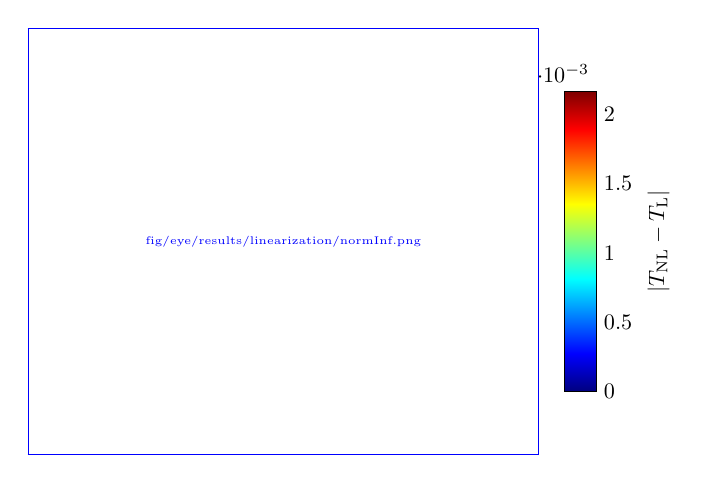
\begin{tikzpicture}[scale=0.8]
        \begin{axis}[
            colorbar,
            colormap/jet, % Choose the colormap you prefer
            % axis equal image,
            enlargelimits=false,
            point meta max=0.002166748046875,
            point meta min=0,
            axis line style = {draw=none},
            tick style = {draw=none},
            xtick = \empty, ytick = \empty,
            colorbar style={
                ylabel = {$|T_\text{NL} - T_\text{L}|$},
                height=0.7*\pgfkeysvalueof{/pgfplots/parent axis height},
                at={(1.05,0.5)}, % Adjust the position to center vertically
                anchor=west, % Adjust the anchor point
            },
            width=0.8\textwidth
        ]
            \addplot graphics [includegraphics cmd=\pgfimage, xmin=0, xmax=1, ymin=0, ymax=1] {fig/eye/results/linearization/normInf.png};
        \end{axis}
    \end{tikzpicture}
    \caption{Difference of the temperature between the full model and the linearized model, computed on the mesh \texttt{M3} with $\P_2$ elements, and the baseline values $\bar{\mu}$ for the parameters.}
    \label{fig:diffLin}
\end{figure}





\Cref{fig:hf:linear} displays the results of the simulation of the linear model $\Em_\text{L}(\mu)$, for three parameters $\mu$:
$\bar{\mu}$ the baseline value parameters, $\mu_{\text{min}}$ (resp. $\mu_\text{max}$) where each component is the lowest (resp. highest) bound of its range of values.

\begin{figure}
    \centering
    \def\mysize{0.3\textwidth}
    \begin{tabular}{*{3}{c}}
        $\bar{\mu}$ & $\mu_{\text{min}}$ & $\mu_{\text{max}}$\\

        \includegraphics[width=\mysize]{fig/eye/results/toolbox/mubar-linear.png} &
        \includegraphics[width=\mysize]{fig/eye/results/toolbox/mumin-linear.png} &
        \includegraphics[width=\mysize]{fig/eye/results/toolbox/mumax-linear.png} \\

        \multicolumn{3}{c}{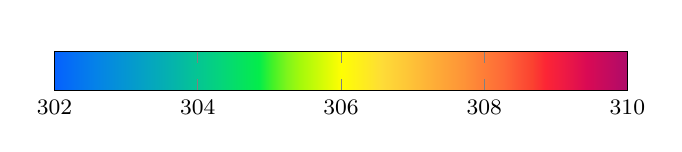
\begin{tikzpicture}
            \begin{axis}[
                colorbar horizontal,
                colormap={blues}{rgb255(0.0cm)=(5,97,254);
                rgb255(0.023809523809523808cm)=(5,108,247);
                rgb255(0.047619047619047616cm)=(5,119,239);
                rgb255(0.07142857142857142cm)=(5,130,232);
                rgb255(0.09523809523809523cm)=(5,139,222);
                rgb255(0.11904761904761904cm)=(5,148,212);
                rgb255(0.14285714285714285cm)=(5,157,202);
                rgb255(0.16666666666666666cm)=(5,166,191);
                rgb255(0.19047619047619047cm)=(5,174,179);
                rgb255(0.21428571428571427cm)=(5,183,167);
                rgb255(0.23809523809523808cm)=(5,193,153);
                rgb255(0.2619047619047619cm)=(5,202,140);
                rgb255(0.2857142857142857cm)=(5,211,126);
                rgb255(0.30952380952380953cm)=(5,220,109);
                rgb255(0.3333333333333333cm)=(5,228,91);
                rgb255(0.35714285714285715cm)=(4,237,74);
                rgb255(0.38095238095238093cm)=(69,242,39);
                rgb255(0.40476190476190477cm)=(125,245,28);
                rgb255(0.42857142857142855cm)=(164,249,11);
                rgb255(0.4523809523809524cm)=(194,251,8);
                rgb255(0.47619047619047616cm)=(224,252,5);
                rgb255(0.5cm)=(254,254,3);
                rgb255(0.5238095238095238cm)=(254,243,20);
                rgb255(0.5476190476190477cm)=(254,232,37);
                rgb255(0.5714285714285714cm)=(254,220,55);
                rgb255(0.5952380952380952cm)=(254,208,55);
                rgb255(0.6190476190476191cm)=(254,196,55);
                rgb255(0.6428571428571429cm)=(254,183,55);
                rgb255(0.6666666666666666cm)=(254,171,55);
                rgb255(0.6904761904761905cm)=(254,159,55);
                rgb255(0.7142857142857143cm)=(254,147,55);
                rgb255(0.7380952380952381cm)=(254,132,55);
                rgb255(0.7619047619047619cm)=(254,118,55);
                rgb255(0.7857142857142857cm)=(254,104,55);
                rgb255(0.8095238095238095cm)=(253,84,53);
                rgb255(0.8333333333333334cm)=(251,66,48);
                rgb255(0.8571428571428571cm)=(252,37,53);
                rgb255(0.8809523809523809cm)=(242,29,64);
                rgb255(0.9047619047619048cm)=(230,20,74);
                rgb255(0.9285714285714286cm)=(218,10,84);
                rgb255(0.9523809523809523cm)=(203,11,91);
                rgb255(0.9761904761904762cm)=(189,11,98);
                rgb255(1.0cm)=(174,12,105);},
                colorbar style={
                    width=0.6\textwidth,
                    % xlabel={Colorbar Label},
                    tick label style={font=\footnotesize},
                },
                ymin=0, ymax=1,
                point meta min=302,
                point meta max=310,
                axis lines=none,
            ]
                \addplot [draw=none] coordinates {(302,0) (310,0)};
            \end{axis}
        \end{tikzpicture}}
    \end{tabular}
    \caption{Distribution of the temperature [\unit{\kelvin}] in the eyeball from the linear model $\Em_\text{L}(\mu)$.}
    \label{fig:hf:linear}
\end{figure}







\subsubsection{Verifications of the reduced basis model}

We compare the results of the reduced basis method with the output of the high fidelity FEM model.
We generate a sample $\Xi_\test$ of 100 parameters in $\Dmu$.
For $\mu\in\Xi_\test$, we compute on the one hand $T_O^\fem(\mu)$, the value of the temperature at point $O$ from the model $\Em_\text{L}(\mu)$,
and on the other hand $T_O^{\rbm, N}(\mu)$, the value of the temperature for the reduced basis model, with a basis of size $N$.
In \Cref{fig:fem-vs-rbm:error}, the value of the error $|T_O^\fem(\mu) - T_O^{\rbm, N}(\mu)|$ is plotted for each $\mu\in\Xi_\test$,
for various reduced basis sizes $N$.
Statistics on the error committed over the sample $\Xi_\test$ are displayed in \Cref{fig:fem-vs-rbm:stats},
as well as the effectivity $\eta_N(\mu)$ in \Cref{fig:fem-vs-rbm:effectivity}.


We observe that even for small values of $N$, the error on the output is remarkably small: an error of $10^{-4}$ is reached for $N=6$.
On the other hand, we find that the convergence on the output is twice as fast as the convergence on the field,
as predicted by the theoretical error estimate \cite[Eq. (36)]{10.1115/1.1448332}.

Note that the anticipated error behavior aligns with theory when the output functional maintains continuity.
In this work, we deviate from the standard case, attributed to the utilization of the Dirac functional in output computation used for pointwise evaluation.
Nevertheless, a similar behavior is observed, and additional insights into this phenomenon will be provided in future work.


\begin{figure}
    \centering
    \def\scl{1}
    \subfigure[Error on RBM for various reduced basis sizes with error bound $\Delta_N^s(\mu)$ \label{fig:fem-vs-rbm:error}]{
        % This file was created with tikzplotly version 0.1.0.
\begin{tikzpicture}[scale=\scl]

\definecolor{3cf210509b}{RGB}{0,128,0}
\definecolor{bc8ae11743}{RGB}{128,0,128}
\definecolor{763bd53097}{RGB}{255,0,0}
\definecolor{416c48ee9e}{RGB}{0,0,255}
\definecolor{5efb101de4}{RGB}{255,165,0}

\pgfplotstableread[col sep=comma]{\currfiledir/data/pointO_errorOnOutput.csv}\val
\pgfplotstableread[col sep=comma]{\currfiledir/data/pointO_errorBound.csv}\err


\begin{axis}[
  % title=Convergence of the RBM,
  xlabel={$T_O^\fem$ [K]},
  ylabel={$|T_O^\fem - T_O^{\rbm, N}|$ [K]},
  ymode=log,
  xmin=289.99322094635886, xmax=306.57046532302854,
  legend columns=5,
  transpose legend,
  legend style={
    fill opacity=0.8,
    draw opacity=1,
    text opacity=1,
    at={(1.03,1.0)},
    anchor=north west
  },
]

  \path[name path=axis] (axis cs:289.99322094635886,1e-9) -- (axis cs:306.57046532302854,1e-9);

  \addplot+ [only marks, name path=N2, mark=*, opacity=0.5, mark options={solid, fill=763bd53097, color=763bd53097}]
    table [col sep=comma, x=T_fem, y=2]
    {\val};
  \addlegendentry{$N=2$}

  \addplot+ [mark=none, name path=error2, opacity=0.2, forget plot]
    table [col sep=comma, x=T_fem, y=2]
    {\err};

  \addplot+ [only marks, name path=N4, mark=*, opacity=0.5, mark options={solid, fill=416c48ee9e, color=416c48ee9e}]
    table [col sep=comma, x=T_fem, y=4]
    {\val};
  \addlegendentry{$N=4$}

  \addplot+ [mark=none, name path=error4, opacity=0.2, forget plot]
    table [col sep=comma, x=T_fem, y=4]
    {\err};

  \addplot+ [only marks, name path=N6, mark=*, opacity=0.5, mark options={solid, fill=3cf210509b, color=3cf210509b}]
    table [col sep=comma, x=T_fem, y=6]
    {\val};
  \addlegendentry{$N=6$}

  \addplot+ [mark=none, name path=error6, opacity=0.2, forget plot]
    table [col sep=comma, x=T_fem, y=6]
    {\err};

  \addplot+ [only marks, name path=N8, mark=*, opacity=0.5, mark options={solid, fill=5efb101de4, color=5efb101de4}]
    table [col sep=comma, x=T_fem, y=8]
    {\val};
  \addlegendentry{$N=8$}

  \addplot+ [mark=none, name path=error8, opacity=0.2, forget plot]
    table [col sep=comma, x=T_fem, y=8]
    {\err};

  \addplot+ [only marks, name path=N10, mark=*, opacity=0.5, mark options={solid, fill=bc8ae11743, color=bc8ae11743}]
    table [col sep=comma, x=T_fem, y=10]
    {\val};
  \addlegendentry{$N=10$}

  \addplot+ [mark=none, name path=error10, opacity=0.2, forget plot]
    table [col sep=comma, x=T_fem, y=10]
    {\err};

  \addplot [thick, color=763bd53097, fill=763bd53097, fill opacity=0.2] fill between [of=error2 and error4];
  \addlegendentry{$\Delta_2^s(\mu)$}
  \addplot [thick, color=416c48ee9e, fill=416c48ee9e, fill opacity=0.2] fill between [of=error4 and error6];
  \addlegendentry{$\Delta_4^s(\mu)$}
  \addplot [thick, color=3cf210509b, fill=3cf210509b, fill opacity=0.2] fill between [of=error6 and error8];
  \addlegendentry{$\Delta_6^s(\mu)$}
  \addplot [thick, color=5efb101de4, fill=5efb101de4, fill opacity=0.2] fill between [of=error8 and error10];
  \addlegendentry{$\Delta_8^s(\mu)$}
  \addplot [thick, color=bc8ae11743, fill=bc8ae11743, fill opacity=0.2] fill between [of=error10 and axis];
  \addlegendentry{$\Delta_{10}^s(\mu)$}

\end{axis}
\end{tikzpicture}

    }
    \def\scl{0.88}
    \subfigure[Convergence of the errors on the field and the output on point $O$, for $\mu\in\Xi_\test$, for various reduced basis sizes. The maximal, minimal, and mean values are represented.\label{fig:fem-vs-rbm:stats}]{
        % This file was created with tikzplotlib v0.10.1.
\pgfplotstableread[col sep=comma]{\currfiledir/data/convergence_error_O.csv}\errors
% \pgfplotstablecreatecol[linear regression={y=outputMean}]{regressionO}{\errors}
% \xdef\slopeO{\pgfplotstableregressiona}
% \pgfplotstablecreatecol[linear regression={y=fieldMean}]{regressionField}{\errors}
% \xdef\slopeField{\pgfplotstableregressiona}
\begin{tikzpicture}[scale=\scl]


\begin{axis}[
    log basis y={10},
    tick align=outside,
    tick pos=left,
    x grid style={darkgray176},
    xlabel={$N$},
    xmin=1.6, xmax=10.4,
    xtick style={color=black},
    y grid style={darkgray176},
    ylabel={Error computed},
    ymode=log,
    ytick style={color=black},
    legend style={fill opacity=0.8, draw opacity=1, text opacity=1, draw=lightgray204, nodes={scale=0.8, transform shape}}
]
\addplot [name path=Mmax, semithick, steelblue31119180, mark=none, mark size=3, mark options={solid}, forget plot] table[y=outputMax] {\errors};
\addplot [name path=Mmin, semithick, steelblue31119180, mark=none, mark size=3, mark options={solid}, forget plot] table[y=outputMin] {\errors};
\addplot [name path=Mmean, semithick, steelblue31119180, mark=*, mark size=3, mark options={solid}, dashed, forget plot] table[y=outputMean] {\errors};
\addplot [color=steelblue31119180, fill=steelblue31119180, opacity=0.2] fill between [of=Mmax and Mmin];
\addlegendentry{$|T^\fem_O(\mu) - T^{\rbm, N}_O(\mu)|$}
\addplot+[colorB, draw=none, mark=none, forget plot] table[x=N, y={create col/linear regression={y=outputMean}}]{\errors};
\xdef\slopeO{\pgfplotstableregressiona}

\addplot [name path=MFmax, semithick, forestgreen4416044, mark=none, mark size=3, mark options={solid}, forget plot] table[y=fieldMax] {\errors};
\addplot [name path=MFmin, semithick, forestgreen4416044, mark=none, mark size=3, mark options={solid}, forget plot] table[y=fieldMin] {\errors};
\addplot [name path=MFmean, semithick, forestgreen4416044, mark=*, mark size=3, mark options={solid}, dashed, forget plot] table[y=fieldMean] {\errors};
\addplot [color=forestgreen4416044, fill=forestgreen4416044, opacity=0.2] fill between [of=MFmax and MFmin];
\addlegendentry{$\norm{T^\fem(\mu) - T^{\rbm, N}(\mu)}{\mu}$}
\addplot+[colorB, draw=none, mark=none, forget plot] table[x=N, y={create col/linear regression={y=fieldMean}}]{\errors};
\xdef\slopeField{\pgfplotstableregressiona}


\logLogSlopeTriangle{0.15}{0.1}{0.2}{\slopeO}{steelblue31119180}
\logLogSlopeTriangle{0.15}{0.1}{0.1}{\slopeField}{forestgreen4416044}



\end{axis}

\end{tikzpicture}

    }
    \subfigure[Stability of the effectivity $\eta_N^s(\mu) = \frac{\Delta_N^s(\mu)}{|T^\fem_O(\mu) - T^{\rbm, N}_O(\mu)|}$ and $\eta_N^\text{en}(\mu) = \frac{\Delta_N^\text{en}(\mu)}{\norm{T^\fem(\mu) - T^{\rbm, N}(\mu)}{\mu}}$ for $\mu\in\Xi_\test$, for various reduced basis sizes. The full red line represents the theoretical lower bound of the effectivity, \textrm{i.e.\ } 1.\label{fig:fem-vs-rbm:effectivity}]{
        % This file was created with tikzplotlib v0.10.1.
\begin{tikzpicture}[scale=\scl]

\definecolor{darkgray176}{RGB}{176,176,176}


\begin{axis}[
log basis y={10},
tick align=outside,
tick pos=left,
x grid style={darkgray176},
xlabel={$N$},
xmin=1.6, xmax=10.4,
xtick style={color=black},
y grid style={darkgray176},
ylabel={$\eta_N(\mu)$},
ymode=log,
ytick style={color=black},
legend style={fill opacity=0.8, draw opacity=1, text opacity=1, draw=lightgray204}
]
\addplot [name path=Mmax, semithick, steelblue31119180, mark=none, mark size=3, mark options={solid}, forget plot]
table {%
2 1066.8884150652973
4 275.5130537402244
6 5175.283748411159
8 227.51000861915077
10 327.78324189653006
};
\addplot [name path=Mmin, semithick, steelblue31119180, mark=none, mark size=3, mark options={solid}, forget plot]
table {%
2 3.6036293609127763
4 4.409972845317161
6 2.769743503906592
8 2.918187278624139
10 5.222510930047634
};
\addplot [name path=Mmean, semithick, steelblue31119180, mark=*, mark size=3, mark options={solid}, dashed, forget plot]
table {%
2 38.83312731510946
4 13.689024117830636
6 87.9511500702313
8 16.080183702477342
10 15.459982089346433
};
\addplot [color=steelblue31119180, fill=steelblue31119180, opacity=0.2] fill between [of=Mmax and Mmin];
\addlegendentry{$\eta_N^s(\mu)$}


\addplot [name path=MFmax, semithick, forestgreen4416044, mark=none, mark size=3, mark options={solid}, forget plot]
table {%
2 1.5343413306443425
4 1.4774853602885867
6 1.4666194896909972
8 1.4666340697067723
10 1.5079660029253543
};
\addplot [name path=MFmin, semithick, forestgreen4416044, mark=none, mark size=3, mark options={solid}, forget plot]
table {%
2 1.3528010083235558
4 1.3138862049682665
6 1.2603680389132252
8 1.3041573261775927
10 1.2920726294213412
};
\addplot [name path=MFmean, semithick, forestgreen4416044, mark=*, mark size=3, mark options={solid}, dashed, forget plot]
table {%
2 1.439823770140758
4 1.4082529053910926
6 1.407758311277011
8 1.3879751517983197
10 1.4039526659084272
};
\addplot [color=forestgreen4416044, fill=forestgreen4416044, opacity=0.2] fill between [of=MFmax and MFmin];
\addlegendentry{$\eta_N^\text{en}(\mu)$}

\addplot[mark=none, red, samples=2] table {
    1.6 1
    10.4 1
};
\end{axis}

\end{tikzpicture}

    }

    \caption{Comparison of the temperature between the full order model and the reduced basis model, tested over a sample $\Xi_\test\subset\Dmu$ of 100 parameters.
    }
    \label{fig:fem-vs-rbm}
\end{figure}



\Cref{tab:time-execution} offers a comparative analysis of execution times for solving the heat transfer problem.
We first discuss the execution times for the high-fidelity solution, encompassing both $\P_1$ and $\P_2$  finite-element discretizations.
The measured time, denoted as $t_\text{exec}$, includes assembling and solving the problem.
In contrast, we also evaluate the execution time of the online phase of our certified reliable reduced basis model.
This comparison highlights a significant reduction in the time required to assemble and solve the problem using our advanced reduced basis approach.
Importantly, this efficiency does not compromise accuracy; the results from the reduced basis model are effectively exact with respect to the high fidelity model.
As anticipated in our earlier scalability analysis, we achieve remarkable computational gains with our model, reinforcing the benefits of our approach in both precision and performance.


\begin{table}
    \centering
    \begin{tabular}{*{5}{c}}
        \toprule
                        & \multicolumn{3}{c}{Finite element resolution}                                    & Reduced model \\
                        & \multicolumn{3}{c}{$T^\fem(\mu)$}                                                & $T^{\rbm, N}(\mu), \Delta_N(\mu)$ \\
        \cmidrule(lr){2-4}
        \cmidrule(lr){5-5}
                        & $\P_1$               & $\P_2$ (\texttt{np=1})         &  $\P_2$ (\texttt{np=12})  &  \\
        \midrule
        Problem size    & $\N = 207~845$       & \multicolumn{2}{c}{$\N = 1~580~932$}                       & $N = 10$ \\
        $t_\text{exec}$ & \qty{5.534}{\second} & \qty{62.432}{\second}          & \qty{10.76}{\second}      & \qty{2.88e-04}{\second}\\
        speed-up        & 11.69                & 1                              & 5.80                      & \textbf{\qty[text-series-to-math]{2.17e5}{}}\\
        \bottomrule
    \end{tabular}
    \caption{Times of execution, using mesh \texttt{M3} for high fidelity simulations.}
    \label{tab:time-execution}
\end{table}


The reduced bases constructed for the various outputs of interest are generated with the greedy algorithm (\Cref{algo:Greedy}),
using a maximal tolerance $\varepsilon_\tol=\pgfmathprintnumber{1e-6}$ and a maximal size for the basis $N = 20$.
In practice, the tolerance is reached for $N = 10$ to 12.




%! TeX root=../article.heat-fom-rom-sa.ijnmbe24.tex
\subsection{Validation and comparison with previous studies}
\label{sec:validation}

We present in this section a thorough comparison between the results of this work and previously published data on the temperature of the eye,
obtained either by experimental procedures or via computational modeling.
Note that only scarce data are available for the entire human eyeball, since most of the measurement techniques estimated only the surface temperature of the cornea.
In particular, \cite{Efron1989OcularST} gathers the outputs of 19 studies conducted with various instruments (mercury bulbs, liquid crystal thermometers or infrared thermometers),
and the mean value reported, according to \cite{NG2006268}, is $T_O^\text{exp} = \qty{307.15}{\kelvin}$.
The temperature at the center of the cornea computed with baseline value from our model is $T_O^\fem(\bar{\mu}) = \pgfmathprintnumber{306.0215598687341}~\unit{\kelvin}$,
which lies in the interval of results found in the literature (see \cite[Table 1]{Efron1989OcularST} and \cite[Table 9]{NG2006268}).

Additionally, in \cite{Efron1989OcularST}, the temperature is measured along an imaginary horizontal line, the \emph{Geometrical Center of the Cornea} (GCC), as described in \Cref{fig:geo-eye}, on a panel of 21 subjects.
The experimental data are displayed in \Cref{fig:res-gcc}, together with the findings of the present work. %, among the curves obtained by \cite{li2010}.
On the horizontal axis, the distance to the center of the eye is represented, and on the vertical axis is the temperature difference to the central one (mean value and standard deviation).
Note that as the geometry of the simulated eye is not the same as the one used in the experiment, we scaled the results over the $x$-axis.
The result shows that the high fidelity model is able to closely replicate the same behavior as the one experimentally measured,
and the model $\Em_\text{L}(\bar{\mu})$ provides very close values (see \Cref{sec:linearized-model}).
Moreover, thanks to the error bound introduced in \Cref{sec:rbm-error-estimates} for the RBM, the approach is considered to be valid for the sensitivity analysis procedure hereafter.


\pgfplotstableread[col sep=comma]{fig/eye/results/GCC/gcc_efron.csv}\gccEfron
\pgfplotstableread[col sep=comma]{fig/eye/results/GCC/gccFeelFullP2.csv}\gccfeel
\pgfplotstableread[col sep=comma]{fig/eye/results/GCC/gcc_li_3D.csv}\gccli

\begin{figure}
    \centering
    \begin{tikzpicture}[trim axis left, trim axis right]
        \begin{axis}
        [legend style = { at = {(1.05,1)}, anchor=north west, nodes={scale=1, transform shape}},
        xlabel = {Distance to center [\unit{\cm}]}, ylabel = {Difference of temperature [\unit{\kelvin}]}, grid = both,
        xmin=-1.2e-2, xmax=1.2e-2, domain=-1e-2:1e-2,
        scaled x ticks={real:1e-2}, xtick scale label code/.code={\,}
        ]
        \addplot+[colorB, mark=none, line width=1pt, opacity=0.4, forget plot] {10807.7*x*x + 0.999464*x};
        \addplot+[colorB, only marks, mark=+, line width=1pt, mark size=4pt] table[col sep=comma,x=dx, y=mean_difference] {\gccEfron};
        \addlegendentry{Measured values \cite{Efron1989OcularST}}
        \addplot+[colorB!80, only marks, mark=+, line width=1pt, mark size=4pt, forget plot] plot [error bars/.cd, y dir=both, y explicit]
            table[col sep=comma,x=dx, y=mean_difference, y error plus=std_up, y error minus=std_down] {\gccEfron};

        \addplot+[colorFeel3, mark=none, line width=1pt, mark size=4pt] table[col sep=comma,x=dx_scaled, y=dT] {\gccfeel};
        \addlegendentry{$\Em_\text{NL}^\N(\bar{\mu}) \equiv \Em_\text{L}^\N(\bar{\mu})$ model}

        \end{axis}
    \end{tikzpicture}
    \caption{Temperature on the GCC: experimental data (mean and standard deviation) vs. numerical results. In this analysis, we cannot distinguish graphical difference between the linear and non-linear models.}
    \label{fig:res-gcc}

\end{figure}





In \Cref{fig:res:line}, we present a comparative analysis between the results of our current study and various numerical findings reported in existing literature.
This comparison features temperatures calculated along a line traversing the eye’s center, the specific location of which is depicted in \Cref{fig:outputs}.
This comparative approach is crucial as it verifies the accuracy of our computed values, encompassing not just the corneal surface but also the eye’s internal tissue structures.
It is noteworthy that our analysis includes a mix of both 2D and 3D results, derived from both non-linear and linearized models.


\begin{figure}
    \centering
    \input{fig/eye/results/line/line.tikz}
    \caption{Temperature on a line going through the center of the eye (see \Cref{fig:outputs}), comparison with numerical results from literature.}
    \label{fig:res:line}
\end{figure}

The results show a very good agreement between the findings of the present study and previously reported temperature results,
along the different locations in the eyeball.


% 4. Uncertainty quantificationœ
%!TeX root=../article.heat-fom-rom-sa.ijnmbe24.tex
\section{Uncertainty quantification}
\label{sec:uq}


The \emph{uncertainty quantification} (UQ) allows quantifying the uncertainty of the model parameters on various outputs.
In the present work, we focus on forward UQ, that is, we want to quantify the uncertainty and the sensitivity of the output of the model, given the uncertainty of the input parameters.
More precisely, two studies are performed:
(i) an uncertainty propagation, to understand how the uncertainties of the inputs of the model are propagated to the output via the computational model, and
(ii) a \emph{sensitivity analysis} (SA) to assess the impact of varying selected parameters on several outputs of interest, namely temperature at specific locations in the eye.
Their locations are detailed in \Cref{fig:outputs}.

The SA is conducted in two different approaches.
First, to recapitulate findings from the literature, we performed a deterministic SA, where for each simulation,
only one parameter is allowed to vary in a given range, whereas the others are fixed to their baseline value.
In a second stage, we extended the SA to a stochastic framework, where each selected parameter follows a given random distribution
and the impact on the quantity of interest is assessed via sensitivity indices.
The advantage of the latter is the global perspective provided by this method and its ability to capture high-order interactions among several input parameters.

% The parameters and their baseline value have been presented in \Cref{sec:parameters}.
% The output of interest for the ocular model is the temperature in specific locations.
% Their locations are detailed in \Cref{fig:outputs}.




\def\ech{0.62}
\begin{figure}
    \centering
    \subfigure[Evaporation rate $E$]{
    \begin{tikzpicture}[scale=\ech]
    \begin{axis}
        [grid=major, xlabel = {$E$ [\unit{\watt.\meter^{-2}}]}, ylabel = {$T$ [\unit{\kelvin}]},
        yticklabel style={scaled ticks=false, /pgf/number format/fixed, /pgf/number format/precision=0},
        xticklabel style={scaled ticks=false, /pgf/number format/fixed, /pgf/number format/precision=0}]
        \addplot[colorFeel3, mark=x, line width=1pt] table[x=E, y=OK, col sep=comma] {fig/eye/results/deterministic-SA/E_feel_K.csv};
        \addplot[colorOoi, mark=square, line width=1pt] table[x=E, y=OK, col sep=comma] {fig/eye/results/deterministic-SA/E_ooi_K.csv};
        \addplot[colorScott, mark=+, line width=1pt] table[x=E, y=OK, col sep=comma] {fig/eye/results/deterministic-SA/E_scott_K.csv};
        \addplot[colorLi, mark=asterisk, line width=1pt] table[x=E, y=OK, col sep=comma] {fig/eye/results/deterministic-SA/E_li_K.csv};
    \draw[dashed, color=black!60, line width=2pt] (40, \pgfkeysvalueof{/pgfplots/ymin}) -- (40, \pgfkeysvalueof{/pgfplots/ymax});
    % \draw[dashed, color=red] (20, \pgfkeysvalueof{/pgfplots/ymin}) -- (20, \pgfkeysvalueof{/pgfplots/ymax});
    % \draw[dashed, color=red] (100, \pgfkeysvalueof{/pgfplots/ymin}) -- (100, \pgfkeysvalueof{/pgfplots/ymax});
    \end{axis}
    \end{tikzpicture}
    }
    \subfigure[Ambient convective coefficient $h_\text{amb}$]{
    \begin{tikzpicture}[scale=\ech]
    \begin{axis}
        [grid=major, xlabel = {$h_\text{amb}$ [\unit{\watt.\meter^{-2}.\kelvin^{-1}}]}, ylabel = {$T$ [\unit{\kelvin}]},
        yticklabel style={scaled ticks=false, /pgf/number format/fixed, /pgf/number format/precision=0},
        xticklabel style={scaled ticks=false, /pgf/number format/fixed, /pgf/number format/precision=0}]
        \addplot[colorFeel3, mark=x, line width=1pt] table[x=h_amb, y=OK, col sep=comma] {fig/eye/results/deterministic-SA/h_amb_feel_K.csv};
        \addplot[colorOoi, mark=square, line width=1pt] table[x=h_amb, y=OK, col sep=comma] {fig/eye/results/deterministic-SA/h_amb_ooi_K.csv};
        \addplot[colorScott, mark=+, line width=1pt] table[x=h_amb, y=OK, col sep=comma] {fig/eye/results/deterministic-SA/h_amb_scott_K.csv};
        \addplot[colorLi, mark=asterisk, line width=1pt] table[x=h_amb, y=OK, col sep=comma] {fig/eye/results/deterministic-SA/h_amb_li_K.csv};
    \draw[dashed, color=black!60, line width=2pt] (10, \pgfkeysvalueof{/pgfplots/ymin}) -- (10, \pgfkeysvalueof{/pgfplots/ymax});
    % \draw[dashed, color=red] (8, \pgfkeysvalueof{/pgfplots/ymin}) -- (8, \pgfkeysvalueof{/pgfplots/ymax});
    % \draw[dashed, color=red] (15, \pgfkeysvalueof{/pgfplots/ymin}) -- (15, \pgfkeysvalueof{/pgfplots/ymax});
    \end{axis}
    \end{tikzpicture}
    }
    \subfigure[Blood convection coefficient $h_\text{bl}$]{
    \begin{tikzpicture}[scale=\ech]
    \begin{axis}
        [grid=major, , xlabel = {$h_\text{bl}$ [\unit{\watt.\meter^{-2}.\kelvin^{-1}}]}, ylabel = {$T$ [\unit{\kelvin}]},
        yticklabel style={scaled ticks=false, /pgf/number format/fixed, /pgf/number format/precision=1},
        xticklabel style={scaled ticks=false, /pgf/number format/fixed, /pgf/number format/precision=0}]
        \addplot[colorFeel3, mark=x, line width=1pt] table[x=h_bl, y=OK, col sep=comma] {fig/eye/results/deterministic-SA/h_bl_feel_K.csv};
        \addplot[colorOoi, mark=square, line width=1pt] table[x=h_bl, y=OK, col sep=comma] {fig/eye/results/deterministic-SA/h_bl_ooi_K.csv};
        \addplot[colorScott, mark=+, line width=1pt] table[x=h_bl, y=OK, col sep=comma] {fig/eye/results/deterministic-SA/h_bl_scott_K.csv};
        \addplot[colorLi, mark=asterisk, line width=1pt] table[x=h_bl, y=OK, col sep=comma] {fig/eye/results/deterministic-SA/h_bl_li_K.csv};
    \draw[dashed, color=black!60, line width=2pt] (65, \pgfkeysvalueof{/pgfplots/ymin}) -- (65, \pgfkeysvalueof{/pgfplots/ymax});
    % \draw[dashed, color=red] (65, \pgfkeysvalueof{/pgfplots/ymin}) -- (65, \pgfkeysvalueof{/pgfplots/ymax});
    % \draw[dashed, color=red] (110, \pgfkeysvalueof{/pgfplots/ymin}) -- (110, \pgfkeysvalueof{/pgfplots/ymax});
    \end{axis}
    \end{tikzpicture}
    }
    \subfigure[Conductivity of the lens $k_\text{lens}$]{
    \begin{tikzpicture}[scale=\ech]
    \begin{axis}
        [grid=major, , xlabel = {$k_\text{lens}$ [\unit{\watt.\meter^{-1}.\kelvin^{-1}}]}, ylabel = {$T$ [\unit{\kelvin}]},
        yticklabel style={scaled ticks=false, /pgf/number format/fixed, /pgf/number format/precision=1},
        xticklabel style={scaled ticks=false, /pgf/number format/fixed, /pgf/number format/precision=1}]
        \addplot[colorFeel3, mark=x, line width=1pt] table[x=k_lens, y=OK, col sep=comma] {fig/eye/results/deterministic-SA/k_lens_feel_K.csv};
        \addplot[colorOoi, mark=square, line width=1pt] table[x=k_lens, y=OK, col sep=comma] {fig/eye/results/deterministic-SA/k_lens_ooi_K.csv};
        \addplot[colorScott, mark=+, line width=1pt] table[x=k_lens, y=OK, col sep=comma] {fig/eye/results/deterministic-SA/k_lens_scott_K.csv};
    \draw[dashed, color=black!60, line width=2pt] (0.4, \pgfkeysvalueof{/pgfplots/ymin}) -- (0.4, \pgfkeysvalueof{/pgfplots/ymax});
    % \draw[dashed, color=red] (0.21, \pgfkeysvalueof{/pgfplots/ymin}) -- (0.21, \pgfkeysvalueof{/pgfplots/ymax});
    % \draw[dashed, color=red] (0.544, \pgfkeysvalueof{/pgfplots/ymin}) -- (0.544, \pgfkeysvalueof{/pgfplots/ymax});
    \end{axis}
    \end{tikzpicture}
    }
    \subfigure[Ambient temperature $T_\text{amb}$]{
    \begin{tikzpicture}[scale=\ech]
    \begin{axis}
        [grid=major, , xlabel = {$T_\text{amb}$ [\unit{\degreeCelsius}]}, ylabel = {$T$ [\unit{\kelvin}]},
        yticklabel style={scaled ticks=false, /pgf/number format/fixed, /pgf/number format/precision=0},
        xticklabel style={scaled ticks=false, /pgf/number format/fixed, /pgf/number format/precision=0}]
        \addplot[colorFeel3, mark=x, line width=1pt] table[x=T_amb, y=OK, col sep=comma] {fig/eye/results/deterministic-SA/T_amb_feel_K.csv};
        \addplot[colorOoi, mark=square, line width=1pt] table[x=T_amb, y=OK, col sep=comma] {fig/eye/results/deterministic-SA/T_amb_ooi_K.csv};
        \addplot[colorScott, mark=+, line width=1pt] table[x=T_amb, y=OK, col sep=comma] {fig/eye/results/deterministic-SA/T_amb_scott_K.csv};
        \addplot[colorLi, mark=asterisk, line width=1pt] table[x=T_amb, y=OK, col sep=comma] {fig/eye/results/deterministic-SA/T_amb_li_K.csv};
    \draw[dashed, color=black!60, line width=2pt] (20, \pgfkeysvalueof{/pgfplots/ymin}) -- (20, \pgfkeysvalueof{/pgfplots/ymax});
    % \draw[dashed, color=red] (10, \pgfkeysvalueof{/pgfplots/ymin}) -- (10, \pgfkeysvalueof{/pgfplots/ymax});
    % \draw[dashed, color=red] (30, \pgfkeysvalueof{/pgfplots/ymin}) -- (30, \pgfkeysvalueof{/pgfplots/ymax});
    \end{axis}
    \end{tikzpicture}
    }
    \subfigure[Blood temperature $T_\text{bl}$]{
    \begin{tikzpicture}[scale=\ech]
    \begin{axis}
        [grid=major, xlabel = {$T_\text{bl}$ [\unit{\degreeCelsius}]}, ylabel = {$T$ [\unit{\kelvin}]},
        yticklabel style={scaled ticks=false, /pgf/number format/fixed, /pgf/number format/precision=0},
        xticklabel style={scaled ticks=false, /pgf/number format/fixed, /pgf/number format/precision=0}]
        \addplot[colorFeel3, mark=x, line width=1pt] table[x=T_bl, y=OK, col sep=comma] {fig/eye/results/deterministic-SA/T_bl_feel_K.csv};
        \addplot[colorOoi, mark=square, line width=1pt] table[x=T_bl, y=OK, col sep=comma] {fig/eye/results/deterministic-SA/T_bl_ooi_K.csv};
        \addplot[colorScott, mark=+, line width=1pt] table[x=T_bl, y=OK, col sep=comma] {fig/eye/results/deterministic-SA/T_bl_scott_K.csv};
        \addplot[colorLi, mark=asterisk, line width=1pt] table[x=T_bl, y=OK, col sep=comma] {fig/eye/results/deterministic-SA/T_bl_li_K.csv};
    \draw[thick, dashed, color=black!60, line width=2pt]  (37, \pgfkeysvalueof{/pgfplots/ymin}) -- (37, \pgfkeysvalueof{/pgfplots/ymax});
    % \draw[dashed, color=red] (35.15, \pgfkeysvalueof{/pgfplots/ymin}) -- (35.15, \pgfkeysvalueof{/pgfplots/ymax});
    % \draw[dashed, color=red] (38.85, \pgfkeysvalueof{/pgfplots/ymin}) -- (38.85, \pgfkeysvalueof{/pgfplots/ymax});
    \end{axis}
    \end{tikzpicture}
    }

    \caption{Results of the DSA for the 6 parameters studied, among previous studies from the literature
        (markers \textcolor{colorFeel3}{\textsf{x} $\Em_\text{NL}(\mu)$}, \textcolor{colorOoi}{$\square$ \cite{NG2006268}}, \textcolor{colorScott}{\textsf{+} \cite{Scott_1988}}, \textcolor{colorLi}{$\ast$ \cite{li2010}}).
        The vertical dashed line corresponds to the baseline value of the parameter.}
    \label{fig:det-sa}
\end{figure}

% This section aims at determining the input parameters that are the most sensitive to the output selected.
% This is done in two different ways, a deterministic sensitivity analysis where only one parameter is allowed to vary while all the others are set to their baseline value and a stochastic sensitivity analysis where each parameter follows a given random distribution.


\subsection{Deterministic sensitivity analysis}
\label{sec:DSA}

Our initial investigation of the impact of varying selected parameters is conducted through a \emph{deterministic sensitivity analysis} (DSA).
Specifically, we choose a parameter among the ones defined in \Cref{tab:parameters}, and we set the other to their baseline value.
Next, we vary the selected parameter among pre-defined values and compute the outputs of the high fidelity model.
Similar studies were performed in \cite{Scott_1988, NG2006268, li2010}.
We gather in the present study information about several parameters of interest for the heat transfer model from these studies,
namely baseline values and ranges.
These variations correspond not only to physiological conditions but also include some extreme situations.
We postpone a more in-depth discussion on this topic to \Cref{sec:SSA}, where the random distributions characterizing these parameters are set up.
Note that in this case, we do not need to use the reduced model, since only a relatively small number of simulations is required.

In \Cref{fig:det-sa}, we show the results of the DSA for the parameter $\mu=\{E, h_\text{amb}, h_\text{bl}, k_\text{lens}, T_\text{amb}, T_\text{bl}\}$, on point $O$ which is at the surface of the cornea.
The plain-line curves correspond to the results reported in the literature, which we compare with the results of our simulations;
the vertical dashed line corresponds to the baseline value for each parameter.
The results are in very good agreement with previous findings and show that temperature at the level of the cornea is strongly influenced by  $h_\text{amb}$, $T_\text{amb}$, $E$, and $T_\text{bl}$,
whereas the influence of $h_\text{bl}$ and $k_\text{lens}$ is less significant.
For instance, high air conductivity can result in a temperature \qty{7}{\kelvin} lower than the baseline value,
while the difference obtained for $h_\text{bl}$ and $k_\text{lens}$ in the computed temperature is at most of \qty{1}{\kelvin}.






\subsection[Stochastic sensitivity analysis]{Stochastic sensitivity analysis (SSA)}
\label{sec:SSA}

We consider an output quantity $Y$ depending on a set of input parameters $\mu\in\Dmu$,
and we estimate the sensitivity of $Y$ to each parameter $\mu_i$ for $i\in\llbracket 1,d\rrbracket$, where $d$ is the dimension of the parametric space.
To this end, we compute the \emph{Sobol' sensitivity indices} introduced in \cite{Sobol1993SensitivityEF} as follows.
We assume that each component $\mu_i$ of $\mu$ follows a random variable $X_i$, independent of the others.
The first-order indices are defined as:

\begin{equation}
    S_i := \frac{\var\left(\E\left[Y\middle|X_i\right]\right)}{\var(Y)}
\end{equation}
where $\var(Y)$ corresponds to the variance of $Y$ including the eventual non-linearity effect of the coefficient on the output,
and $\var\left(\E\left[Y\middle|X_i\right]\right)$ is the variance of the conditional expectation of $Y$ given $X_i$, corresponding to the first order effect of the parameter $\mu_i$ on the output:
if the parameter modeled by the distribution $X_j$ has a great impact on the output $Y$, then $\E\left[Y\middle|X_j\right]$ will vary has well, and so its variance.

We also define the \emph{total Sobol' index}:

\begin{equation}
    S_i^\text{tot} := \frac{\var\left(\E\left[Y\middle|X_{(-i)}\right]\right)}{\var(Y)} = 1 - S_{-i}
\end{equation}
where $X_{(-i)} = (X_1,\cdots,X_{i-1},X_{i+1},\cdots,X_d)$ is the set of parameters without the parameter $X_i$, and $S_{-i}$ is the sum of the indices where $X_i$ is not present.

% We may also introduce Sobol's indices of higher order, to estimate the impact of coupled parameters on the output, but as we will see in the results this is not necessary.

To compute the Sobol' indices, we use an algorithm of functional chaos, implemented in the library OpenTURNS \cite{Baudin2016} by the class \texttt{FunctionalChaosAlgorithm}, using a bootstrap method%
\footnote{See documentation \url{https://openturns.github.io/openturns/latest/auto_meta_modeling/polynomial_chaos_metamodel/plot_chaos_sobol_confidence.html}}
for the confidence intervals.



\subsubsection{Choice of the distributions}

We discuss now the prior distributions for each parameter.
Each parameter does not depend on the others, resulting in a family of 6 random independent variables.
\Cref{fig:eye:distributions} shows the probability density function (PDF) of distributions of the parameters,
associated with the baseline values (see \Cref{tab:parameters}),
where the parameters used in the literature for the deterministic sensitivity analysis are represented with a vertical line.
We present hereafter some details on how the random distributions were constructed.


\begin{itemize}
    \item \textbf{Evaporation rate $E$:} According to \cite{Scott_1988}, the evaporation rate's range is of 40 to 100 \unit{\watt.\meter^{-2}}, using data from literature \cite{adler53}.
    The value $E=\qty{40}{\watt.\meter^{-2}}$ is chosen as the baseline value.
    Some high values are also considered, to study the impact of important evaporation rates.
    The values used in the literature run from 20 to \qty{320}{\watt.\meter^{-2}}.
    As this parameter varies by several orders of magnitude, we decided to use a log-normal distribution to represent it.
    More precisely we set $E\sim \logN(\mu_E, \sigma_E, \gamma_E)$, with $\sigma_E = 0.7$, $\mu_E=\log(40)-\frac{0.15^2}{2}$ and $\gamma_E=20$, restricted to $[20, 130]$.
    The distribution is presented in \Cref{fig:eye:distributions:E}.
    This choice of the distribution leads to a mean value of $\overline{E}=\qty{55.8}{\watt.\meter^{-2}}$.

    \item \textbf{Ambient air convection coefficient $h_\text{\normalfont amb}$:}
    In \cite{Scott_1988}, the sole value given for the ambient air convection coefficient is \qty{10}{\watt.\meter^{-2}.\kelvin^{-1}}, and similar values are used to run the DSA, from 8 to 15~\unit{\watt.\meter^{-2}.\kelvin^{-1}}.
    Other results in the literature coroborate this value: \cite[Table 12.2]{KOSKY2013259} reports a range of 2.5 to 25~\unit{\watt.\meter^{-2}.\kelvin^{-1}} for a free convection, and 10 to \qty{500}{\watt.\meter^{-2}.\kelvin^{-1}} for a forced convection.
    \cite{engeneer-edge} proposes a range of 10 to \qty{100}{\watt.\meter^{-2}.\kelvin^{-1}} for the air.
    In their DSA, \cite{NG2006268} and \cite{li2010} use higher values of $h_\text{amb}$, up to \qty{100}{\watt.\meter^{-2}.\kelvin^{-1}} to simulate a forced convection condition.
    As high values are not a common case, such a coefficient should not have a high frequency in the distribution.
    We chose to use a log-normal distribution: $h_\text{amb}\sim \logN\left(\log(10)-\frac{1}{2}, 1, 8\right)$.
    In Remark \ref{rem:linearization}, we discussed the linearization process of the model, inducing the usage of a fixed parameter $h_\text{r}$ chosen to fit temperature in usual ambient room conditions,
    which leads to a restriction of the distribution to the interval $[8, 100]~\unit{\watt.\meter^{-2}.\kelvin^{-1}}$.
    The distribution is presented in \Cref{fig:eye:distributions:hamb}.
    The mean value of the distribution is $\overline{h_\text{amb}}=\qty{17.6}{\watt.\meter^{-2}.\kelvin^{-1}}$.

    \item \textbf{Blood convection coefficient $h_\text{\normalfont bl}$:} A control value of \qty{65}{\watt.\meter^{-2}.\kelvin^{-1}}, derived from experimental data \cite{Lagendijk_1982} is provided in \cite{Scott_1988}.
    For the DSA, the values used run from 50 to \qty{120}{\watt.\meter^{-2}.\kelvin^{-1}}.
    This leads us to the following assumption for the distribution of the parameter: $h_\text{bl}\sim \logN\left(\log(65)-\frac{0.15^2}{2}, 0.15, 0\right)$, restricted over $[50, 120]$, see \Cref{fig:eye:distributions:hbl}.
    The mean of this distribution is $\overline{h_\text{bl}}=\qty{65.8}{\watt.\meter^{-2}.\kelvin^{-1}}$.

    \item \textbf{Lens conductivity $k_\text{\normalfont lens}$:} This parameter is chosen among all the conductivities since the water content of the lens varies with aging \cite{Scott_1988}.
    \cite{Scott_1988} and \cite{NG2006268} run the DSA with this parameter, using values from 0.21 to \qty{0.544}{\watt\metre^{-1}\kelvin^{-1}}.
    As the range of values is not very large, it seems reasonable to use a uniform distribution for this parameter: $k_\text{lens}\sim \unif(0.21, 0.544)$, see \Cref{fig:eye:distributions:klens}.

    \item \textbf{Ambient temperature $T_\text{\normalfont amb}$:} The baseline value of this parameter is taken to a usual room temperature of \qty{294}{\kelvin} (\qty{20}{\celsius}).
    The values used for the DSA vary from extreme conditions of \qty{273}{\kelvin} (\qty{0}{\celsius}) to \qty{308}{\kelvin} (\qty{35}{\celsius}).
    As these extreme values are not very common, we choose to restrict the values taken by $T_\text{amb}$ from \qty{283.15}{\kelvin} (\qty{-35}{\celsius}) to \qty{303.15}{\kelvin} (\qty{30}{\celsius}): $T_\text{amb}\sim \unif(283.15, 303.15)$.
    The distribution is presented in \Cref{fig:eye:distributions:Tamb}.

    \item \textbf{Blood temperature $T_\text{\normalfont bl}$:} The temperature of human blood is commonly accepted to be \qty{310}{\kelvin} (\qty{37}{\celsius}).
    For the DSA, cases of hypothermia and hyperthermia are considered, with a range from \qtyrange{308}{312.15}{\kelvin} (\qtyrange{35}{39}{\celsius}).
    We therefore take $T_\text{bl}\sim \unif(308, 312.15)$, see \Cref{fig:eye:distributions:Tbl}.
\end{itemize}



\begin{figure}
    \centering
    \def\chl{0.6}
    \subfigure[Distribution of $E$\label{fig:eye:distributions:E}]{
        % This file was created with tikzplotlib v0.10.1.
\begin{tikzpicture}[scale=\chl]

\definecolor{darkgray176}{RGB}{176,176,176}
\definecolor{darkorange25512714}{RGB}{255,127,14}
\definecolor{forestgreen4416044}{RGB}{44,160,44}
\definecolor{lightgray204}{RGB}{204,204,204}
\definecolor{steelblue31119180}{RGB}{31,119,180}

\begin{axis}[
legend cell align={left},
legend style={
  fill opacity=0.8,
  draw opacity=1,
  text opacity=1,
  at={(0.99,0.99)},
  anchor=north east,
  draw=lightgray204,
  nodes={scale=0.8, transform shape}
},
tick align=outside,
tick pos=left,
% title={E},
x grid style={darkgray176},
xlabel={$E$ [\unit{\watt.\meter^{-2}}]},
xmajorgrids,
xmin=-10.7699338462917, xmax=144.959770628964,
xtick style={color=black},
y grid style={darkgray176},
% ymajorticks=false,
% ylabel={PDF},
% ymajorgrids,
ymin=-0.00120604026816441, ymax=0.0253268456314527,
ytick style={color=black}
]
\addplot [dashed, red, fill=red, fill opacity=0.25]
table {%
-22.7822200065073 0
-21.534139719041 0
-20.2860594315747 0
-19.0379791441084 0
-17.7898988566421 0
-16.5418185691758 0
-15.2937382817095 0
-14.0456579942432 0
-12.7975777067768 0
-11.5494974193105 0
-10.3014171318442 0
-9.05333684437793 0
-7.80525655691162 0
-6.55717626944531 0
-5.30909598197901 0
-4.0610156945127 0
-2.8129354070464 0
-1.56485511958009 0
-0.316774832113783 0
0.931305455352522 0
2.17938574281883 0
3.42746603028514 0
4.67554631775144 0
5.92362660521775 0
7.17170689268405 0
8.41978718015036 0
9.66786746761667 0
10.915947755083 0
12.1640280425493 0
13.4121083300156 0
14.6601886174819 0
15.9082689049482 0
17.1563491924145 0
18.4044294798808 0
19.6525097673471 0
20.9005900548134 1.72547435768853e-06
22.1486703422797 0.000181582907477345
23.396750629746 0.00113414561660361
24.6448309172123 0.00310025379771601
25.8929112046786 0.00582684483753852
27.140991492145 0.00891274264757005
28.3890717796113 0.012010746463036
29.6371520670776 0.0148833462960416
30.8852323545439 0.0173946663405769
32.1333126420102 0.019484687905207
33.3813929294765 0.0211438273972586
34.6294732169428 0.0223930668785405
35.8775535044091 0.0232699726949402
37.1256337918754 0.0238194826100309
38.3737140793417 0.024088157572697
39.621794366808 0.0241208053632883
40.8698746542743 0.023958663398171
42.1179549417406 0.023638571637223
43.3660352292069 0.0231927515183586
44.6141155166732 0.0226489384553381
45.8621958041395 0.0220307056935559
47.1102760916058 0.0213578777587736
48.3583563790722 0.0206469714956011
49.6064366665385 0.0199116284495652
50.8545169540048 0.0191630187683871
52.1025972414711 0.018410207071761
53.3506775289374 0.0176604770060341
54.5987578164037 0.0169196148843155
55.84683810387 0.0161921548523157
57.0949183913363 0.0154815890300633
58.3429986788026 0.0147905464588627
59.5910789662689 0.0141209446887326
60.8391592537352 0.0134741176381079
62.0872395412015 0.0128509230478454
63.3353198286678 0.0122518324989238
64.5834001161341 0.0116770066055136
65.8314804036004 0.0111263576537601
67.0795606910667 0.0105996016428447
68.3276409785331 0.0100963014034393
69.5757212659994 0.00961590222049305
70.8238015534657 0.00915776117113344
72.071881840932 0.00872117120189821
73.3199621283983 0.00830538080958581
74.5680424158646 0.00790961005363437
75.8161227033309 0.00753306351210646
77.0642029907972 0.00717494069528157
78.3122832782635 0.00683444434801822
79.5603635657298 0.00651078700220824
80.8084438531961 0.00620319608185311
82.0565241406624 0.00591091781385667
83.3046044281287 0.00563322015609863
84.552684715595 0.00536939491948942
85.8007650030613 0.00511875923145685
87.0488452905277 0.00488065646378603
88.296925577994 0.00465445672717269
89.5450058654603 0.00443955701762145
90.7930861529266 0.00423538108538846
92.0411664403929 0.00404137908508453
93.2892467278592 0.00385702705544022
94.5373270153255 0.00368182626877279
95.7854073027918 0.00351530248311904
97.0334875902581 0.00335700512408507
98.2815678777244 0.00320650641852594
99.5296481651907 0.00306340049804798
100.777728452657 0.00292730248689243
102.025808740123 0.00279784758589962
103.27388902759 0.00267469016187615
104.521969315056 0.00255750284971448
105.770049602522 0.00244597567298067
107.018129889989 0.00233981518733538
108.266210177455 0.00223874365004065
109.514290464921 0.00214249821789144
110.762370752387 0.00205083017516283
112.010451039854 0.00196350419255592
113.25853132732 0.00188029761763203
114.506611614786 0.00180099979682978
115.754691902253 0.00172541142884338
117.002772189719 0.0016533439488925
118.250852477185 0.00158461894322068
119.498932764652 0.00151906759301218
120.747013052118 0.0014565301468076
121.995093339584 0.00139685542042074
123.243173627051 0.00133990032330569
124.491253914517 0.00128552941029182
125.739334201983 0.00123361445758846
126.987414489449 0.00118403406195963
128.235494776916 0.00113667326197789
129.483575064382 0.00109142318028403
130.731655351848 0
131.979735639315 0
133.227815926781 0
134.475896214247 0
135.723976501714 0
136.97205678918 0
};
\addlegendentry{PDF}
\addplot [dashed, color=black!60, line width=2pt]
table {%
40 -0.00120604026816441
40 0.0253268456314527
};
\addlegendentry{Baseline}
\addplot [semithick, colorLi]
table {%
30 -0.00120604026816441
30 0.0253268456314527
};
\addlegendentry{\cite{li2010}}
\addplot [semithick, colorLi, forget plot]
table {%
80 -0.00120604026816441
80 0.0253268456314527
};
\addplot [semithick, colorLi, forget plot]
table {%
130 -0.00120604026816441
130 0.0253268456314527
};
\addplot [semithick, colorLi, forget plot]
table {%
180 -0.00120604026816441
180 0.0253268456314527
};
\addplot [semithick, colorLi, forget plot]
table {%
230 -0.00120604026816441
230 0.0253268456314527
};
\addplot [semithick, colorOoi]
table {%
20 -0.00120604026816441
20 0.0253268456314527
};
\addlegendentry{\cite{NG2006268}}
\addplot [semithick, colorOoi, forget plot]
table {%
40 -0.00120604026816441
40 0.0253268456314527
};
\addplot [semithick, colorOoi, forget plot]
table {%
70 -0.00120604026816441
70 0.0253268456314527
};
\addplot [semithick, colorOoi, forget plot]
table {%
100 -0.00120604026816441
100 0.0253268456314527
};
\addplot [semithick, colorOoi, forget plot]
table {%
320 -0.00120604026816441
320 0.0253268456314527
};
\addplot [semithick, colorScott]
table {%
20 -0.00120604026816441
20 0.0253268456314527
};
\addlegendentry{\cite{Scott_1988}}
\addplot [semithick, colorScott, forget plot]
table {%
40 -0.00120604026816441
40 0.0253268456314527
};
\addplot [semithick, colorScott, forget plot]
table {%
100 -0.00120604026816441
100 0.0253268456314527
};
\addplot [semithick, colorScott, forget plot]
table {%
320 -0.00120604026816441
320 0.0253268456314527
};
\end{axis}

\end{tikzpicture}

    }
    \subfigure[Distribution of $h_\text{amb}$\label{fig:eye:distributions:hamb}]{
        % This file was created with tikzplotlib v0.10.1.
\begin{tikzpicture}[scale=\chl]

\definecolor{darkgray176}{RGB}{176,176,176}
\definecolor{darkorange25512714}{RGB}{255,127,14}
\definecolor{forestgreen4416044}{RGB}{44,160,44}
\definecolor{lightgray204}{RGB}{204,204,204}
\definecolor{steelblue31119180}{RGB}{31,119,180}

\begin{axis}[
legend cell align={left},
legend style={
  fill opacity=0.8,
  draw opacity=1,
  text opacity=1,
  at={(0.99,0.99)},
  anchor=north east,
  draw=lightgray204,
  nodes={scale=0.8, transform shape}
},
tick align=outside,
tick pos=left,
% title={h\_amb},
x grid style={darkgray176},
xlabel={$h_\text{amb}$ [\unit{\watt.\meter^{-2}.\kelvin^{-1}}]},
xmajorgrids,
xmin=-10, xmax=110,
xtick style={color=black},
y grid style={darkgray176},
% ymajorticks=false,
% ylabel={PDF},
% ymajorgrids,
ymin=-0.00542153685454793, ymax=0.113852273945507,
ytick style={color=black}
]
\addplot [dashed, red, fill=red, fill opacity=0.25]
table[x=x, y=pdf, col sep=comma] {fig/eye/distributions/h_amb_pdf.csv};
\addlegendentry{PDF}
\addplot [dashed, color=black!60, line width=2pt]
table {%
9.99999999999999 -0.00542153685454794
9.99999999999999 0.113852273945507
};
\addlegendentry{Baseline}
\addplot [semithick, colorLi]
table {%
15 -0.00542153685454794
15 0.113852273945507
};
\addlegendentry{\cite{li2010}}
\addplot [semithick, colorLi, forget plot]
table {%
30 -0.00542153685454794
30 0.113852273945507
};
\addplot [semithick, colorLi, forget plot]
table {%
50 -0.00542153685454794
50 0.113852273945507
};
\addplot [semithick, colorLi, forget plot]
table {%
80 -0.00542153685454794
80 0.113852273945507
};
\addplot [semithick, colorLi, forget plot]
table {%
100 -0.00542153685454794
100 0.113852273945507
};
\addplot [semithick, colorOoi]
table {%
8 -0.00542153685454794
8 0.113852273945507
};
\addlegendentry{\cite{NG2006268}}
\addplot [semithick, colorOoi, forget plot]
table {%
9.99999999999999 -0.00542153685454794
9.99999999999999 0.113852273945507
};
\addplot [semithick, colorOoi, forget plot]
table {%
15 -0.00542153685454794
15 0.113852273945507
};
\addplot [semithick, colorOoi, forget plot]
table {%
100 -0.00542153685454794
100 0.113852273945507
};
\addplot [semithick, colorScott]
table {%
8 -0.00542153685454794
8 0.113852273945507
};
\addlegendentry{\cite{Scott_1988}}
\addplot [semithick, colorScott, forget plot]
table {%
9.99999999999999 -0.00542153685454794
9.99999999999999 0.113852273945507
};
\addplot [semithick, colorScott, forget plot]
table {%
12 -0.00542153685454794
12 0.113852273945507
};
\addplot [semithick, colorScott, forget plot]
table {%
15 -0.00542153685454794
15 0.113852273945507
};
\end{axis}

\end{tikzpicture}

    }
    \subfigure[Distribution of $h_\text{bl}$\label{fig:eye:distributions:hbl}]{
        % This file was created with tikzplotlib v0.10.1.
\begin{tikzpicture}[scale=\chl]

\definecolor{darkgray176}{RGB}{176,176,176}
\definecolor{darkorange25512714}{RGB}{255,127,14}
\definecolor{forestgreen4416044}{RGB}{44,160,44}
\definecolor{lightgray204}{RGB}{204,204,204}
\definecolor{steelblue31119180}{RGB}{31,119,180}

\begin{axis}[
legend cell align={left},
legend style={
  fill opacity=0.8,
  draw opacity=1,
  text opacity=1,
  at={(0.99,0.99)},
  anchor=north east,
  draw=lightgray204,
  nodes={scale=0.8, transform shape}
},
tick align=outside,
tick pos=left,
% title={h\_bl},
x grid style={darkgray176},
xlabel={$h_\text{bl}$ [\unit{\watt.\meter^{-2}.\kelvin^{-1}}]},
xmajorgrids,
xmin=40, xmax=130,
xtick style={color=black},
% ymajorticks=false,
% ylabel={PDF},
% ymajorgrids,
ymin=-0.00219537964264221, ymax=0.0461029724954863,
ytick style={color=black}
]
\addplot [dashed, red, fill=red, fill opacity=0.25]
table[x=x, y=pdf, col sep=comma] {fig/eye/distributions/h_bl_pdf.csv};
\addlegendentry{PDF}
\addplot [dashed, color=black!60, line width=2pt]
table {%
65 -0.00219537964264221
65 0.0461029724954863
};
\addlegendentry{Baseline}
\addplot [semithick, colorLi]
table {%
50 -0.00219537964264221
50 0.0461029724954863
};
\addlegendentry{\cite{li2010}}
\addplot [semithick, colorLi, forget plot]
table {%
70 -0.00219537964264221
70 0.0461029724954863
};
\addplot [semithick, colorLi, forget plot]
table {%
90 -0.00219537964264221
90 0.0461029724954863
};
\addplot [semithick, colorLi, forget plot]
table {%
110 -0.00219537964264221
110 0.0461029724954863
};
\addplot [semithick, colorLi, forget plot]
table {%
120 -0.00219537964264221
120 0.0461029724954863
};
\addplot [semithick, colorOoi]
table {%
65 -0.00219537964264221
65 0.0461029724954863
};
\addlegendentry{\cite{NG2006268}}
\addplot [semithick, colorOoi, forget plot]
table {%
90 -0.00219537964264221
90 0.0461029724954863
};
\addplot [semithick, colorOoi, forget plot]
table {%
110 -0.00219537964264221
110 0.0461029724954863
};
\addplot [semithick, colorScott]
table {%
65 -0.00219537964264221
65 0.0461029724954863
};
\addlegendentry{\cite{Scott_1988}}
\addplot [semithick, colorScott, forget plot]
table {%
90 -0.00219537964264221
90 0.0461029724954863
};
\addplot [semithick, colorScott, forget plot]
table {%
110 -0.00219537964264221
110 0.0461029724954863
};
\end{axis}

\end{tikzpicture}

    }
    \subfigure[Distribution of $k_\text{lens}$\label{fig:eye:distributions:klens}]{
        % This file was created with tikzplotlib v0.10.1.
\begin{tikzpicture}[scale=\chl]

\definecolor{darkgray176}{RGB}{176,176,176}
\definecolor{forestgreen4416044}{RGB}{44,160,44}
\definecolor{lightgray204}{RGB}{204,204,204}

\begin{axis}[
legend cell align={left},
legend style={fill opacity=0.8, draw opacity=1, text opacity=1, draw=lightgray204, nodes={scale=0.7, transform shape}},
tick align=outside,
tick pos=left,
% title={k\_lens},
x grid style={darkgray176},
xlabel={$k_\text{lens}$ [\unit{\watt.\meter^{-1}.\kelvin^{-1}}]},
xmajorgrids,
xmin=-0.0859240000000001, xmax=0.839924,
xtick style={color=black},
y grid style={darkgray176},
% ymajorticks=false,
% ylabel={PDF},
ymajorgrids,
ymin=-0.149700598802395, ymax=3.1437125748503,
ytick style={color=black}
]
\addplot [dashed, red, fill=red, fill opacity=0.25]
table {%
-0.04384 0
-0.037264375 0
-0.03068875 0
-0.024113125 0
-0.0175375 0
-0.010961875 0
-0.00438625000000004 0
0.00218937499999997 0
0.00876499999999997 0
0.015340625 0
0.02191625 0
0.028491875 0
0.0350675 0
0.041643125 0
0.04821875 0
0.054794375 0
0.06137 0
0.067945625 0
0.07452125 0
0.081096875 0
0.0876725 0
0.094248125 0
0.10082375 0
0.107399375 0
0.113975 0
0.120550625 0
0.12712625 0
0.133701875 0
0.1402775 0
0.146853125 0
0.15342875 0
0.160004375 0
0.16658 0
0.173155625 0
0.17973125 0
0.186306875 0
0.1928825 0
0.199458125 0
0.20603375 0
0.212609375 2.9940119760479
0.219185 2.9940119760479
0.225760625 2.9940119760479
0.23233625 2.9940119760479
0.238911875 2.9940119760479
0.2454875 2.9940119760479
0.252063125 2.9940119760479
0.25863875 2.9940119760479
0.265214375 2.9940119760479
0.27179 2.9940119760479
0.278365625 2.9940119760479
0.28494125 2.9940119760479
0.291516875 2.9940119760479
0.2980925 2.9940119760479
0.304668125 2.9940119760479
0.31124375 2.9940119760479
0.317819375 2.9940119760479
0.324395 2.9940119760479
0.330970625 2.9940119760479
0.33754625 2.9940119760479
0.344121875 2.9940119760479
0.3506975 2.9940119760479
0.357273125 2.9940119760479
0.36384875 2.9940119760479
0.370424375 2.9940119760479
0.377 2.9940119760479
0.383575625 2.9940119760479
0.39015125 2.9940119760479
0.396726875 2.9940119760479
0.4033025 2.9940119760479
0.409878125 2.9940119760479
0.41645375 2.9940119760479
0.423029375 2.9940119760479
0.429605 2.9940119760479
0.436180625 2.9940119760479
0.44275625 2.9940119760479
0.449331875 2.9940119760479
0.4559075 2.9940119760479
0.462483125 2.9940119760479
0.46905875 2.9940119760479
0.475634375 2.9940119760479
0.48221 2.9940119760479
0.488785625 2.9940119760479
0.49536125 2.9940119760479
0.501936875 2.9940119760479
0.5085125 2.9940119760479
0.515088125 2.9940119760479
0.52166375 2.9940119760479
0.528239375 2.9940119760479
0.534815 2.9940119760479
0.541390625 2.9940119760479
0.54796625 0
0.554541875 0
0.5611175 0
0.567693125 0
0.57426875 0
0.580844375 0
0.58742 0
0.593995625 0
0.60057125 0
0.607146875 0
0.6137225 0
0.620298125 0
0.62687375 0
0.633449375 0
0.640025 0
0.646600625 0
0.65317625 0
0.659751875 0
0.6663275 0
0.672903125 0
0.67947875 0
0.686054375 0
0.69263 0
0.699205625 0
0.70578125 0
0.712356875 0
0.7189325 0
0.725508125 0
0.73208375 0
0.738659375 0
0.745235 0
0.751810625 0
0.75838625 0
0.764961875 0
0.7715375 0
0.778113125 0
0.78468875 0
0.791264375 0
0.79784 0
};
\addlegendentry{PDF}
\addplot [dashed, color=black!60, line width=2pt]
table {%
0.4 -0.149700598802395
0.4 3.1437125748503
};
\addlegendentry{Baseline}
\addplot [semithick, forestgreen4416044, dashed]
table {%
0.21 -0.149700598802395
0.21 3.1437125748503
};
\addlegendentry{\cite{NG2006268} \& \cite{Scott_1988}}
\addplot [semithick, forestgreen4416044, dashed, forget plot]
table {%
0.3 -0.149700598802395
0.3 3.1437125748503
};
\addplot [semithick, forestgreen4416044, dashed, forget plot]
table {%
0.4 -0.149700598802395
0.4 3.1437125748503
};
\addplot [semithick, forestgreen4416044, dashed, forget plot]
table {%
0.544 -0.149700598802395
0.544 3.1437125748503
};
\end{axis}

\end{tikzpicture}

    }
    \subfigure[Distribution of $T_\text{amb}$\label{fig:eye:distributions:Tamb}]{
        % This file was created with tikzplotlib v0.10.1.
\begin{tikzpicture}[scale=\chl]

\definecolor{darkgray176}{RGB}{176,176,176}
\definecolor{darkorange25512714}{RGB}{255,127,14}
\definecolor{forestgreen4416044}{RGB}{44,160,44}
\definecolor{lightgray204}{RGB}{204,204,204}
\definecolor{steelblue31119180}{RGB}{31,119,180}

\begin{axis}[
legend cell align={left},
legend style={fill opacity=0.8, draw opacity=1, text opacity=1, draw=lightgray204, nodes={scale=0.7, transform shape}},
tick align=outside,
tick pos=left,
% title={T\_amb},
x grid style={darkgray176},
xlabel={$T_\text{amb}$ [\unit{\kelvin}]},
xmajorgrids,
xmin=265.43, xmax=320.87,
xtick style={color=black},
y grid style={darkgray176},
% ylabel={PDF},
% ymajorticks=false,
ymajorgrids,
ymin=-0.0025, ymax=0.0525,
ytick style={color=black}
]
\addplot [dashed, red, fill=red, fill opacity=0.25]
table {%
267.95 0
268.34375 0
268.7375 0
269.13125 0
269.525 0
269.91875 0
270.3125 0
270.70625 0
271.1 0
271.49375 0
271.8875 0
272.28125 0
272.675 0
273.06875 0
273.4625 0
273.85625 0
274.25 0
274.64375 0
275.0375 0
275.43125 0
275.825 0
276.21875 0
276.6125 0
277.00625 0
277.4 0
277.79375 0
278.1875 0
278.58125 0
278.975 0
279.36875 0
279.7625 0
280.15625 0
280.55 0
280.94375 0
281.3375 0
281.73125 0
282.125 0
282.51875 0
282.9125 0
283.30625 0.05
283.7 0.05
284.09375 0.05
284.4875 0.05
284.88125 0.05
285.275 0.05
285.66875 0.05
286.0625 0.05
286.45625 0.05
286.85 0.05
287.24375 0.05
287.6375 0.05
288.03125 0.05
288.425 0.05
288.81875 0.05
289.2125 0.05
289.60625 0.05
290 0.05
290.39375 0.05
290.7875 0.05
291.18125 0.05
291.575 0.05
291.96875 0.05
292.3625 0.05
292.75625 0.05
293.15 0.05
293.54375 0.05
293.9375 0.05
294.33125 0.05
294.725 0.05
295.11875 0.05
295.5125 0.05
295.90625 0.05
296.3 0.05
296.69375 0.05
297.0875 0.05
297.48125 0.05
297.875 0.05
298.26875 0.05
298.6625 0.05
299.05625 0.05
299.45 0.05
299.84375 0.05
300.2375 0.05
300.63125 0.05
301.025 0.05
301.41875 0.05
301.8125 0.05
302.20625 0.05
302.6 0.05
302.99375 0.05
303.3875 0
303.78125 0
304.175 0
304.56875 0
304.9625 0
305.35625 0
305.75 0
306.14375 0
306.5375 0
306.93125 0
307.325 0
307.71875 0
308.1125 0
308.50625 0
308.9 0
309.29375 0
309.6875 0
310.08125 0
310.475 0
310.86875 0
311.2625 0
311.65625 0
312.05 0
312.44375 0
312.8375 0
313.23125 0
313.625 0
314.01875 0
314.4125 0
314.80625 0
315.2 0
315.59375 0
315.9875 0
316.38125 0
316.775 0
317.16875 0
317.5625 0
317.95625 0
318.35 0
};
\addlegendentry{PDF}
\addplot [dashed, color=black!60, line width=2pt]
table {%
294 -0.0025
294 0.0525
};
\addlegendentry{Baseline}
\addplot [semithick, colorLi]
table {%
273 -0.0025
273 0.0525
};
\addlegendentry{\cite{li2010}}
\addplot [semithick, colorLi, forget plot]
table {%
278 -0.0025
278 0.0525
};
\addplot [semithick, colorLi, forget plot]
table {%
283 -0.0025
283 0.0525
};
\addplot [semithick, colorLi, forget plot]
table {%
303 -0.0025
303 0.0525
};
\addplot [semithick, colorLi, forget plot]
table {%
308 -0.0025
308 0.0525
};
\addplot [semithick, colorOoi]
table {%
293.15 -0.0025
293.15 0.0525
};
\addlegendentry{\cite{NG2006268} \& \cite{Scott_1988}}
\addplot [semithick, colorOoi, forget plot]
table {%
298.15 -0.0025
298.15 0.0525
};
\addplot [semithick, colorOoi, forget plot]
table {%
303.15 -0.0025
303.15 0.0525
};
% \addplot [semithick, colorScott]
% table {%
% 293.15 -0.0025
% 293.15 0.0525
% };
% \addlegendentry{\cite{Scott_1988}}
% \addplot [semithick, colorScott, forget plot]
% table {%
% 298.15 -0.0025
% 298.15 0.0525
% };
% \addplot [semithick, colorScott, forget plot]
% table {%
% 303.15 -0.0025
% 303.15 0.0525
% };
\end{axis}

\end{tikzpicture}

    }
    \subfigure[Distribution of $T_\text{bl}$\label{fig:eye:distributions:Tbl}]{
        % This file was created with tikzplotlib v0.10.1.
\begin{tikzpicture}[scale=\chl]

\definecolor{darkgray176}{RGB}{176,176,176}
\definecolor{darkorange25512714}{RGB}{255,127,14}
\definecolor{forestgreen4416044}{RGB}{44,160,44}
\definecolor{lightgray204}{RGB}{204,204,204}
\definecolor{steelblue31119180}{RGB}{31,119,180}

\begin{axis}[
legend cell align={left},
legend style={fill opacity=0.8, draw opacity=1, text opacity=1, draw=lightgray204, nodes={scale=0.6, transform shape}},
tick align=outside,
tick pos=left,
% title={$T_bl$},
x grid style={darkgray176},
xlabel={$T_\text{bl}$ [\unit{\kelvin}]},
xmajorgrids,
xmin=304.3231, xmax=315.8269,
xtick style={color=black},
y grid style={darkgray176},
% ymajorticks=false,
% ylabel={PDF},
ymin=-0.0120481927710844, ymax=0.253012048192772,
ytick style={color=black}
]
\addplot [dashed, red, fill=red, fill opacity=0.25]
table {%
304.846 0
304.927703125 0
305.00940625 0
305.091109375 0
305.1728125 0
305.254515625 0
305.33621875 0
305.417921875 0
305.499625 0
305.581328125 0
305.66303125 0
305.744734375 0
305.8264375 0
305.908140625 0
305.98984375 0
306.071546875 0
306.15325 0
306.234953125 0
306.31665625 0
306.398359375 0
306.4800625 0
306.561765625 0
306.64346875 0
306.725171875 0
306.806875 0
306.888578125 0
306.97028125 0
307.051984375 0
307.1336875 0
307.215390625 0
307.29709375 0
307.378796875 0
307.4605 0
307.542203125 0
307.62390625 0
307.705609375 0
307.7873125 0
307.869015625 0
307.95071875 0
308.032421875 0.240963855421688
308.114125 0.240963855421688
308.195828125 0.240963855421688
308.27753125 0.240963855421688
308.359234375 0.240963855421688
308.4409375 0.240963855421688
308.522640625 0.240963855421688
308.60434375 0.240963855421688
308.686046875 0.240963855421688
308.76775 0.240963855421688
308.849453125 0.240963855421688
308.93115625 0.240963855421688
309.012859375 0.240963855421688
309.0945625 0.240963855421688
309.176265625 0.240963855421688
309.25796875 0.240963855421688
309.339671875 0.240963855421688
309.421375 0.240963855421688
309.503078125 0.240963855421688
309.58478125 0.240963855421688
309.666484375 0.240963855421688
309.7481875 0.240963855421688
309.829890625 0.240963855421688
309.91159375 0.240963855421688
309.993296875 0.240963855421688
310.075 0.240963855421688
310.156703125 0.240963855421688
310.23840625 0.240963855421688
310.320109375 0.240963855421688
310.4018125 0.240963855421688
310.483515625 0.240963855421688
310.56521875 0.240963855421688
310.646921875 0.240963855421688
310.728625 0.240963855421688
310.810328125 0.240963855421688
310.89203125 0.240963855421688
310.973734375 0.240963855421688
311.0554375 0.240963855421688
311.137140625 0.240963855421688
311.21884375 0.240963855421688
311.300546875 0.240963855421688
311.38225 0.240963855421688
311.463953125 0.240963855421688
311.54565625 0.240963855421688
311.627359375 0.240963855421688
311.7090625 0.240963855421688
311.790765625 0.240963855421688
311.87246875 0.240963855421688
311.954171875 0.240963855421688
312.035875 0.240963855421688
312.117578125 0.240963855421688
312.19928125 0
312.280984375 0
312.3626875 0
312.444390625 0
312.52609375 0
312.607796875 0
312.6895 0
312.771203125 0
312.85290625 0
312.934609375 0
313.0163125 0
313.098015625 0
313.17971875 0
313.261421875 0
313.343125 0
313.424828125 0
313.50653125 0
313.588234375 0
313.6699375 0
313.751640625 0
313.83334375 0
313.915046875 0
313.99675 0
314.078453125 0
314.16015625 0
314.241859375 0
314.3235625 0
314.405265625 0
314.48696875 0
314.568671875 0
314.650375 0
314.732078125 0
314.81378125 0
314.895484375 0
314.9771875 0
315.058890625 0
315.14059375 0
315.222296875 0
315.304 0
};
\addlegendentry{PDF}
\addplot [dashed, color=black!60, line width=2pt]
table {%
310 -0.0120481927710844
310 0.253012048192772
};
\addlegendentry{Baseline}
\addplot [semithick, colorLi]
table {%
308 -0.0120481927710844
308 0.253012048192772
};
\addplot [semithick, colorLi, forget plot]
table {%
309 -0.0120481927710844
309 0.253012048192772
};
\addplot [semithick, colorLi, forget plot]
table {%
310 -0.0120481927710844
310 0.253012048192772
};
\addplot [semithick, colorLi, forget plot]
table {%
311 -0.0120481927710844
311 0.253012048192772
};
\addplot [semithick, colorLi, forget plot]
table {%
312 -0.0120481927710844
312 0.253012048192772
};
\addlegendentry{\cite{li2010}}
\addplot [semithick, colorOoi]
table {%
308.15 -0.0120481927710844
308.15 0.253012048192772
};
\addplot [semithick, colorOoi, forget plot]
table {%
310.15 -0.0120481927710844
310.15 0.253012048192772
};
\addplot [semithick, colorOoi, forget plot]
table {%
311.15 -0.0120481927710844
311.15 0.253012048192772
};
\addplot [semithick, colorOoi, forget plot]
table {%
312.15 -0.0120481927710844
312.15 0.253012048192772
};
\addlegendentry{\cite{NG2006268}}
\addplot [semithick, colorScott]
table {%
310.15 -0.0120481927710844
310.15 0.253012048192772
};
\addplot [semithick, colorScott, dashed, forget plot]
table {%
310.95 -0.0120481927710844
310.95 0.253012048192772
};
\addplot [semithick, colorScott, dashed, forget plot]
table {%
311.15 -0.0120481927710844
311.15 0.253012048192772
};
\addplot [semithick, colorScott, dashed, forget plot]
table {%
311.65 -0.0120481927710844
311.65 0.253012048192772
};
\addlegendentry{\cite{Scott_1988}}
\end{axis}

\end{tikzpicture}

    }
    \caption{Distributions of the parameters. The vertical lines represent the values chosen in literature for the DSA.}
    \label{fig:eye:distributions}
\end{figure}


\subsubsection{Uncertainty propagation}

We focus on the distribution of outputs of interest, from a random sample of the input parameters of get from the distributions presented $\pgfmathprintnumber{10000}$ points, which leads to a number of $\pgfmathprintnumber{10000}$ simulations.
The computational cost of the high fidelity simulations becomes in this case prohibitive and therefore we employ the reduced basis metamodel developed in \Cref{sec:rbm}.
\Cref{fig:uncertainty-propagation} presents the distribution of three outputs, namely the mean of the temperature over the cornea $T_\text{cornea}$,
and the temperature on points $O$ and $G$ respectively are the front and the back of the eyeball.
Note that $T_O$ and $T_\text{cornea}$ display a Gaussian distribution, whereas $T_G$ is more difficult to interpret, but could correspond to a uniform or bi-modal distribution.



We provide in \Cref{tab:results:uncertainty-propagation} results about mean values and standard deviation for the same quantities.
We note that the mean values of $T_O$ and $T_\text{cornea}$ are of the same order of magnitude as the experimental data in the validation section (\Cref{sec:validation}): the difference of temperature is about \qty{2}{\kelvin}, and standard deviations are in the same ranges.
The mean value of $T_G$ is very close to results reported in \Cref{fig:res:line} from the literature with a small standard deviation.

\begin{table}
    \centering
    \begin{tabular}{cccc}
        \toprule
        & $T_\text{cornea}$ & $T_O$ & $T_G$ \\
        \midrule
        Mean & 305.590082 & 303.185187 & 310.028526 \\
        Standard deviation & 1.788358 & 2.457063 & 1.055978 \\
        \bottomrule
    \end{tabular}
    \caption{Statistics of the outputs.}
    \label{tab:results:uncertainty-propagation}
\end{table}


\begin{figure}
    \centering
    % This file was created with tikzplotlib v0.10.1.
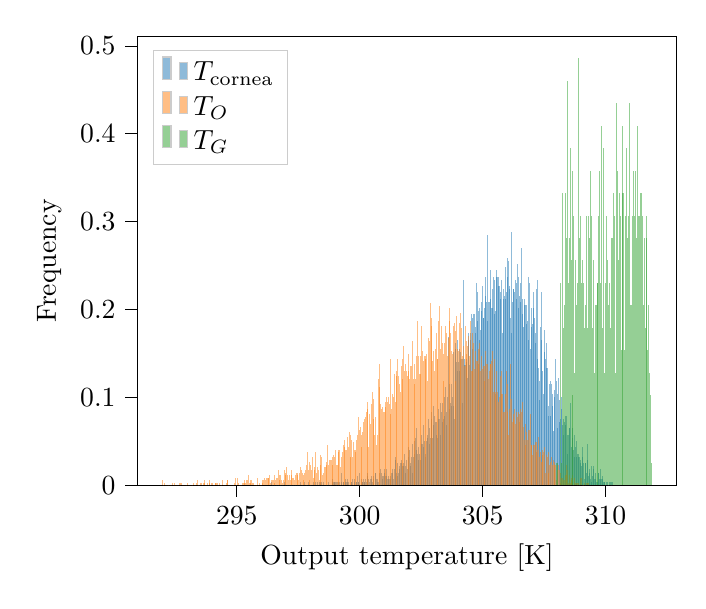
\begin{tikzpicture}

\definecolor{darkgray176}{RGB}{176,176,176}
\definecolor{darkorange25512714}{RGB}{255,127,14}
\definecolor{lightgray204}{RGB}{204,204,204}
\definecolor{steelblue31119180}{RGB}{31,119,180}

\begin{axis}[
legend cell align={left},
legend style={
    fill opacity=0.8,
    draw opacity=1,
    text opacity=1,
    at={(0.03,0.97)},
    anchor=north west,
    draw=lightgray204
},
tick align=outside,
tick pos=left,
x grid style={darkgray176},
xmin=290.947304577462, xmax=312.897909705608,
xtick style={color=black},
y grid style={darkgray176},
ymin=0, ymax=0.510177905708991,
ytick style={color=black},
xlabel={Output temperature [K]},
ylabel={Frequency},
]
\draw[draw=none,fill=steelblue31119180,fill opacity=0.5] (axis cs:296.385624126556,0) rectangle (axis cs:296.413422588011,0.00359732138999415);
\addlegendimage{ybar,ybar legend,draw=none,fill=steelblue31119180,fill opacity=0.5}
\addlegendentry{$T_\text{cornea}$}

\draw[draw=none,fill=steelblue31119180,fill opacity=0.5] (axis cs:296.413422588011,0) rectangle (axis cs:296.441221049466,0);
\draw[draw=none,fill=steelblue31119180,fill opacity=0.5] (axis cs:296.441221049466,0) rectangle (axis cs:296.469019510921,0);
\draw[draw=none,fill=steelblue31119180,fill opacity=0.5] (axis cs:296.469019510921,0) rectangle (axis cs:296.496817972375,0);
\draw[draw=none,fill=steelblue31119180,fill opacity=0.5] (axis cs:296.496817972375,0) rectangle (axis cs:296.52461643383,0);
\draw[draw=none,fill=steelblue31119180,fill opacity=0.5] (axis cs:296.52461643383,0) rectangle (axis cs:296.552414895285,0);
\draw[draw=none,fill=steelblue31119180,fill opacity=0.5] (axis cs:296.552414895285,0) rectangle (axis cs:296.58021335674,0);
\draw[draw=none,fill=steelblue31119180,fill opacity=0.5] (axis cs:296.58021335674,0) rectangle (axis cs:296.608011818194,0);
\draw[draw=none,fill=steelblue31119180,fill opacity=0.5] (axis cs:296.608011818194,0) rectangle (axis cs:296.635810279649,0);
\draw[draw=none,fill=steelblue31119180,fill opacity=0.5] (axis cs:296.635810279649,0) rectangle (axis cs:296.663608741104,0);
\draw[draw=none,fill=steelblue31119180,fill opacity=0.5] (axis cs:296.663608741104,0) rectangle (axis cs:296.691407202558,0);
\draw[draw=none,fill=steelblue31119180,fill opacity=0.5] (axis cs:296.691407202558,0) rectangle (axis cs:296.719205664013,0);
\draw[draw=none,fill=steelblue31119180,fill opacity=0.5] (axis cs:296.719205664013,0) rectangle (axis cs:296.747004125468,0);
\draw[draw=none,fill=steelblue31119180,fill opacity=0.5] (axis cs:296.747004125468,0) rectangle (axis cs:296.774802586923,0);
\draw[draw=none,fill=steelblue31119180,fill opacity=0.5] (axis cs:296.774802586923,0) rectangle (axis cs:296.802601048378,0);
\draw[draw=none,fill=steelblue31119180,fill opacity=0.5] (axis cs:296.802601048377,0) rectangle (axis cs:296.830399509832,0);
\draw[draw=none,fill=steelblue31119180,fill opacity=0.5] (axis cs:296.830399509832,0) rectangle (axis cs:296.858197971287,0);
\draw[draw=none,fill=steelblue31119180,fill opacity=0.5] (axis cs:296.858197971287,0) rectangle (axis cs:296.885996432742,0);
\draw[draw=none,fill=steelblue31119180,fill opacity=0.5] (axis cs:296.885996432742,0) rectangle (axis cs:296.913794894196,0);
\draw[draw=none,fill=steelblue31119180,fill opacity=0.5] (axis cs:296.913794894196,0) rectangle (axis cs:296.941593355651,0.00359732138999415);
\draw[draw=none,fill=steelblue31119180,fill opacity=0.5] (axis cs:296.941593355651,0) rectangle (axis cs:296.969391817106,0);
\draw[draw=none,fill=steelblue31119180,fill opacity=0.5] (axis cs:296.969391817106,0) rectangle (axis cs:296.997190278561,0);
\draw[draw=none,fill=steelblue31119180,fill opacity=0.5] (axis cs:296.997190278561,0) rectangle (axis cs:297.024988740015,0);
\draw[draw=none,fill=steelblue31119180,fill opacity=0.5] (axis cs:297.024988740015,0) rectangle (axis cs:297.05278720147,0);
\draw[draw=none,fill=steelblue31119180,fill opacity=0.5] (axis cs:297.05278720147,0) rectangle (axis cs:297.080585662925,0);
\draw[draw=none,fill=steelblue31119180,fill opacity=0.5] (axis cs:297.080585662925,0) rectangle (axis cs:297.10838412438,0);
\draw[draw=none,fill=steelblue31119180,fill opacity=0.5] (axis cs:297.10838412438,0) rectangle (axis cs:297.136182585834,0);
\draw[draw=none,fill=steelblue31119180,fill opacity=0.5] (axis cs:297.136182585834,0) rectangle (axis cs:297.163981047289,0);
\draw[draw=none,fill=steelblue31119180,fill opacity=0.5] (axis cs:297.163981047289,0) rectangle (axis cs:297.191779508744,0);
\draw[draw=none,fill=steelblue31119180,fill opacity=0.5] (axis cs:297.191779508744,0) rectangle (axis cs:297.219577970199,0);
\draw[draw=none,fill=steelblue31119180,fill opacity=0.5] (axis cs:297.219577970199,0) rectangle (axis cs:297.247376431653,0);
\draw[draw=none,fill=steelblue31119180,fill opacity=0.5] (axis cs:297.247376431653,0) rectangle (axis cs:297.275174893108,0);
\draw[draw=none,fill=steelblue31119180,fill opacity=0.5] (axis cs:297.275174893108,0) rectangle (axis cs:297.302973354563,0);
\draw[draw=none,fill=steelblue31119180,fill opacity=0.5] (axis cs:297.302973354563,0) rectangle (axis cs:297.330771816018,0);
\draw[draw=none,fill=steelblue31119180,fill opacity=0.5] (axis cs:297.330771816018,0) rectangle (axis cs:297.358570277472,0);
\draw[draw=none,fill=steelblue31119180,fill opacity=0.5] (axis cs:297.358570277472,0) rectangle (axis cs:297.386368738927,0);
\draw[draw=none,fill=steelblue31119180,fill opacity=0.5] (axis cs:297.386368738927,0) rectangle (axis cs:297.414167200382,0);
\draw[draw=none,fill=steelblue31119180,fill opacity=0.5] (axis cs:297.414167200382,0) rectangle (axis cs:297.441965661837,0);
\draw[draw=none,fill=steelblue31119180,fill opacity=0.5] (axis cs:297.441965661837,0) rectangle (axis cs:297.469764123291,0);
\draw[draw=none,fill=steelblue31119180,fill opacity=0.5] (axis cs:297.469764123291,0) rectangle (axis cs:297.497562584746,0);
\draw[draw=none,fill=steelblue31119180,fill opacity=0.5] (axis cs:297.497562584746,0) rectangle (axis cs:297.525361046201,0);
\draw[draw=none,fill=steelblue31119180,fill opacity=0.5] (axis cs:297.525361046201,0) rectangle (axis cs:297.553159507656,0);
\draw[draw=none,fill=steelblue31119180,fill opacity=0.5] (axis cs:297.553159507656,0) rectangle (axis cs:297.58095796911,0);
\draw[draw=none,fill=steelblue31119180,fill opacity=0.5] (axis cs:297.58095796911,0) rectangle (axis cs:297.608756430565,0.00359732138999415);
\draw[draw=none,fill=steelblue31119180,fill opacity=0.5] (axis cs:297.608756430565,0) rectangle (axis cs:297.63655489202,0);
\draw[draw=none,fill=steelblue31119180,fill opacity=0.5] (axis cs:297.63655489202,0) rectangle (axis cs:297.664353353474,0);
\draw[draw=none,fill=steelblue31119180,fill opacity=0.5] (axis cs:297.664353353475,0) rectangle (axis cs:297.692151814929,0);
\draw[draw=none,fill=steelblue31119180,fill opacity=0.5] (axis cs:297.692151814929,0) rectangle (axis cs:297.719950276384,0);
\draw[draw=none,fill=steelblue31119180,fill opacity=0.5] (axis cs:297.719950276384,0) rectangle (axis cs:297.747748737839,0.00359732138999415);
\draw[draw=none,fill=steelblue31119180,fill opacity=0.5] (axis cs:297.747748737839,0) rectangle (axis cs:297.775547199293,0);
\draw[draw=none,fill=steelblue31119180,fill opacity=0.5] (axis cs:297.775547199293,0) rectangle (axis cs:297.803345660748,0);
\draw[draw=none,fill=steelblue31119180,fill opacity=0.5] (axis cs:297.803345660748,0) rectangle (axis cs:297.831144122203,0);
\draw[draw=none,fill=steelblue31119180,fill opacity=0.5] (axis cs:297.831144122203,0) rectangle (axis cs:297.858942583658,0);
\draw[draw=none,fill=steelblue31119180,fill opacity=0.5] (axis cs:297.858942583658,0) rectangle (axis cs:297.886741045112,0);
\draw[draw=none,fill=steelblue31119180,fill opacity=0.5] (axis cs:297.886741045112,0) rectangle (axis cs:297.914539506567,0.00359732138998679);
\draw[draw=none,fill=steelblue31119180,fill opacity=0.5] (axis cs:297.914539506567,0) rectangle (axis cs:297.942337968022,0);
\draw[draw=none,fill=steelblue31119180,fill opacity=0.5] (axis cs:297.942337968022,0) rectangle (axis cs:297.970136429477,0);
\draw[draw=none,fill=steelblue31119180,fill opacity=0.5] (axis cs:297.970136429477,0) rectangle (axis cs:297.997934890932,0);
\draw[draw=none,fill=steelblue31119180,fill opacity=0.5] (axis cs:297.997934890931,0) rectangle (axis cs:298.025733352386,0);
\draw[draw=none,fill=steelblue31119180,fill opacity=0.5] (axis cs:298.025733352386,0) rectangle (axis cs:298.053531813841,0);
\draw[draw=none,fill=steelblue31119180,fill opacity=0.5] (axis cs:298.053531813841,0) rectangle (axis cs:298.081330275296,0);
\draw[draw=none,fill=steelblue31119180,fill opacity=0.5] (axis cs:298.081330275296,0) rectangle (axis cs:298.10912873675,0);
\draw[draw=none,fill=steelblue31119180,fill opacity=0.5] (axis cs:298.10912873675,0) rectangle (axis cs:298.136927198205,0.00359732138998679);
\draw[draw=none,fill=steelblue31119180,fill opacity=0.5] (axis cs:298.136927198205,0) rectangle (axis cs:298.16472565966,0);
\draw[draw=none,fill=steelblue31119180,fill opacity=0.5] (axis cs:298.16472565966,0) rectangle (axis cs:298.192524121115,0.00359732138999415);
\draw[draw=none,fill=steelblue31119180,fill opacity=0.5] (axis cs:298.192524121115,0) rectangle (axis cs:298.220322582569,0);
\draw[draw=none,fill=steelblue31119180,fill opacity=0.5] (axis cs:298.220322582569,0) rectangle (axis cs:298.248121044024,0);
\draw[draw=none,fill=steelblue31119180,fill opacity=0.5] (axis cs:298.248121044024,0) rectangle (axis cs:298.275919505479,0);
\draw[draw=none,fill=steelblue31119180,fill opacity=0.5] (axis cs:298.275919505479,0) rectangle (axis cs:298.303717966934,0.00359732138998679);
\draw[draw=none,fill=steelblue31119180,fill opacity=0.5] (axis cs:298.303717966934,0) rectangle (axis cs:298.331516428388,0);
\draw[draw=none,fill=steelblue31119180,fill opacity=0.5] (axis cs:298.331516428388,0) rectangle (axis cs:298.359314889843,0);
\draw[draw=none,fill=steelblue31119180,fill opacity=0.5] (axis cs:298.359314889843,0) rectangle (axis cs:298.387113351298,0.00359732138999415);
\draw[draw=none,fill=steelblue31119180,fill opacity=0.5] (axis cs:298.387113351298,0) rectangle (axis cs:298.414911812753,0.00359732138999415);
\draw[draw=none,fill=steelblue31119180,fill opacity=0.5] (axis cs:298.414911812753,0) rectangle (axis cs:298.442710274207,0.00359732138998679);
\draw[draw=none,fill=steelblue31119180,fill opacity=0.5] (axis cs:298.442710274207,0) rectangle (axis cs:298.470508735662,0);
\draw[draw=none,fill=steelblue31119180,fill opacity=0.5] (axis cs:298.470508735662,0) rectangle (axis cs:298.498307197117,0);
\draw[draw=none,fill=steelblue31119180,fill opacity=0.5] (axis cs:298.498307197117,0) rectangle (axis cs:298.526105658572,0.00359732138998679);
\draw[draw=none,fill=steelblue31119180,fill opacity=0.5] (axis cs:298.526105658572,0) rectangle (axis cs:298.553904120026,0);
\draw[draw=none,fill=steelblue31119180,fill opacity=0.5] (axis cs:298.553904120026,0) rectangle (axis cs:298.581702581481,0);
\draw[draw=none,fill=steelblue31119180,fill opacity=0.5] (axis cs:298.581702581481,0) rectangle (axis cs:298.609501042936,0);
\draw[draw=none,fill=steelblue31119180,fill opacity=0.5] (axis cs:298.609501042936,0) rectangle (axis cs:298.637299504391,0);
\draw[draw=none,fill=steelblue31119180,fill opacity=0.5] (axis cs:298.637299504391,0) rectangle (axis cs:298.665097965845,0);
\draw[draw=none,fill=steelblue31119180,fill opacity=0.5] (axis cs:298.665097965845,0) rectangle (axis cs:298.6928964273,0);
\draw[draw=none,fill=steelblue31119180,fill opacity=0.5] (axis cs:298.6928964273,0) rectangle (axis cs:298.720694888755,0.00359732138999415);
\draw[draw=none,fill=steelblue31119180,fill opacity=0.5] (axis cs:298.720694888755,0) rectangle (axis cs:298.74849335021,0);
\draw[draw=none,fill=steelblue31119180,fill opacity=0.5] (axis cs:298.74849335021,0) rectangle (axis cs:298.776291811664,0);
\draw[draw=none,fill=steelblue31119180,fill opacity=0.5] (axis cs:298.776291811664,0) rectangle (axis cs:298.804090273119,0);
\draw[draw=none,fill=steelblue31119180,fill opacity=0.5] (axis cs:298.804090273119,0) rectangle (axis cs:298.831888734574,0);
\draw[draw=none,fill=steelblue31119180,fill opacity=0.5] (axis cs:298.831888734574,0) rectangle (axis cs:298.859687196028,0);
\draw[draw=none,fill=steelblue31119180,fill opacity=0.5] (axis cs:298.859687196029,0) rectangle (axis cs:298.887485657483,0.00359732138998679);
\draw[draw=none,fill=steelblue31119180,fill opacity=0.5] (axis cs:298.887485657483,0) rectangle (axis cs:298.915284118938,0.0071946427799883);
\draw[draw=none,fill=steelblue31119180,fill opacity=0.5] (axis cs:298.915284118938,0) rectangle (axis cs:298.943082580393,0.00359732138999415);
\draw[draw=none,fill=steelblue31119180,fill opacity=0.5] (axis cs:298.943082580393,0) rectangle (axis cs:298.970881041847,0.00359732138998679);
\draw[draw=none,fill=steelblue31119180,fill opacity=0.5] (axis cs:298.970881041847,0) rectangle (axis cs:298.998679503302,0.00359732138999415);
\draw[draw=none,fill=steelblue31119180,fill opacity=0.5] (axis cs:298.998679503302,0) rectangle (axis cs:299.026477964757,0.00359732138998679);
\draw[draw=none,fill=steelblue31119180,fill opacity=0.5] (axis cs:299.026477964757,0) rectangle (axis cs:299.054276426212,0);
\draw[draw=none,fill=steelblue31119180,fill opacity=0.5] (axis cs:299.054276426212,0) rectangle (axis cs:299.082074887666,0.00359732138999415);
\draw[draw=none,fill=steelblue31119180,fill opacity=0.5] (axis cs:299.082074887666,0) rectangle (axis cs:299.109873349121,0.00359732138998679);
\draw[draw=none,fill=steelblue31119180,fill opacity=0.5] (axis cs:299.109873349121,0) rectangle (axis cs:299.137671810576,0.00359732138999415);
\draw[draw=none,fill=steelblue31119180,fill opacity=0.5] (axis cs:299.137671810576,0) rectangle (axis cs:299.165470272031,0);
\draw[draw=none,fill=steelblue31119180,fill opacity=0.5] (axis cs:299.165470272031,0) rectangle (axis cs:299.193268733485,0.00359732138998679);
\draw[draw=none,fill=steelblue31119180,fill opacity=0.5] (axis cs:299.193268733485,0) rectangle (axis cs:299.22106719494,0);
\draw[draw=none,fill=steelblue31119180,fill opacity=0.5] (axis cs:299.22106719494,0) rectangle (axis cs:299.248865656395,0.0143892855599472);
\draw[draw=none,fill=steelblue31119180,fill opacity=0.5] (axis cs:299.248865656395,0) rectangle (axis cs:299.27666411785,0.00359732138999415);
\draw[draw=none,fill=steelblue31119180,fill opacity=0.5] (axis cs:299.27666411785,0) rectangle (axis cs:299.304462579304,0);
\draw[draw=none,fill=steelblue31119180,fill opacity=0.5] (axis cs:299.304462579304,0) rectangle (axis cs:299.332261040759,0.00359732138998679);
\draw[draw=none,fill=steelblue31119180,fill opacity=0.5] (axis cs:299.332261040759,0) rectangle (axis cs:299.360059502214,0.00359732138999415);
\draw[draw=none,fill=steelblue31119180,fill opacity=0.5] (axis cs:299.360059502214,0) rectangle (axis cs:299.387857963669,0);
\draw[draw=none,fill=steelblue31119180,fill opacity=0.5] (axis cs:299.387857963669,0) rectangle (axis cs:299.415656425123,0.00719464277997358);
\draw[draw=none,fill=steelblue31119180,fill opacity=0.5] (axis cs:299.415656425123,0) rectangle (axis cs:299.443454886578,0.00359732138999415);
\draw[draw=none,fill=steelblue31119180,fill opacity=0.5] (axis cs:299.443454886578,0) rectangle (axis cs:299.471253348033,0.00359732138998679);
\draw[draw=none,fill=steelblue31119180,fill opacity=0.5] (axis cs:299.471253348033,0) rectangle (axis cs:299.499051809488,0.0071946427799883);
\draw[draw=none,fill=steelblue31119180,fill opacity=0.5] (axis cs:299.499051809488,0) rectangle (axis cs:299.526850270942,0.00359732138999415);
\draw[draw=none,fill=steelblue31119180,fill opacity=0.5] (axis cs:299.526850270942,0) rectangle (axis cs:299.554648732397,0.00359732138998679);
\draw[draw=none,fill=steelblue31119180,fill opacity=0.5] (axis cs:299.554648732397,0) rectangle (axis cs:299.582447193852,0);
\draw[draw=none,fill=steelblue31119180,fill opacity=0.5] (axis cs:299.582447193852,0) rectangle (axis cs:299.610245655307,0);
\draw[draw=none,fill=steelblue31119180,fill opacity=0.5] (axis cs:299.610245655307,0) rectangle (axis cs:299.638044116761,0);
\draw[draw=none,fill=steelblue31119180,fill opacity=0.5] (axis cs:299.638044116761,0) rectangle (axis cs:299.665842578216,0.00359732138999415);
\draw[draw=none,fill=steelblue31119180,fill opacity=0.5] (axis cs:299.665842578216,0) rectangle (axis cs:299.693641039671,0.00359732138998679);
\draw[draw=none,fill=steelblue31119180,fill opacity=0.5] (axis cs:299.693641039671,0) rectangle (axis cs:299.721439501126,0.0071946427799883);
\draw[draw=none,fill=steelblue31119180,fill opacity=0.5] (axis cs:299.721439501126,0) rectangle (axis cs:299.74923796258,0);
\draw[draw=none,fill=steelblue31119180,fill opacity=0.5] (axis cs:299.74923796258,0) rectangle (axis cs:299.777036424035,0.00719464277997358);
\draw[draw=none,fill=steelblue31119180,fill opacity=0.5] (axis cs:299.777036424035,0) rectangle (axis cs:299.80483488549,0.00359732138999415);
\draw[draw=none,fill=steelblue31119180,fill opacity=0.5] (axis cs:299.80483488549,0) rectangle (axis cs:299.832633346944,0);
\draw[draw=none,fill=steelblue31119180,fill opacity=0.5] (axis cs:299.832633346944,0) rectangle (axis cs:299.860431808399,0.00359732138998679);
\draw[draw=none,fill=steelblue31119180,fill opacity=0.5] (axis cs:299.860431808399,0) rectangle (axis cs:299.888230269854,0.00359732138999415);
\draw[draw=none,fill=steelblue31119180,fill opacity=0.5] (axis cs:299.888230269854,0) rectangle (axis cs:299.916028731309,0.0107919641699604);
\draw[draw=none,fill=steelblue31119180,fill opacity=0.5] (axis cs:299.916028731309,0) rectangle (axis cs:299.943827192763,0.00359732138999415);
\draw[draw=none,fill=steelblue31119180,fill opacity=0.5] (axis cs:299.943827192763,0) rectangle (axis cs:299.971625654218,0.00359732138999415);
\draw[draw=none,fill=steelblue31119180,fill opacity=0.5] (axis cs:299.971625654218,0) rectangle (axis cs:299.999424115673,0.0143892855599472);
\draw[draw=none,fill=steelblue31119180,fill opacity=0.5] (axis cs:299.999424115673,0) rectangle (axis cs:300.027222577128,0);
\draw[draw=none,fill=steelblue31119180,fill opacity=0.5] (axis cs:300.027222577128,0) rectangle (axis cs:300.055021038582,0);
\draw[draw=none,fill=steelblue31119180,fill opacity=0.5] (axis cs:300.055021038582,0) rectangle (axis cs:300.082819500037,0.00719464277997358);
\draw[draw=none,fill=steelblue31119180,fill opacity=0.5] (axis cs:300.082819500037,0) rectangle (axis cs:300.110617961492,0.00359732138999415);
\draw[draw=none,fill=steelblue31119180,fill opacity=0.5] (axis cs:300.110617961492,0) rectangle (axis cs:300.138416422947,0.00359732138999415);
\draw[draw=none,fill=steelblue31119180,fill opacity=0.5] (axis cs:300.138416422947,0) rectangle (axis cs:300.166214884401,0.00719464277997358);
\draw[draw=none,fill=steelblue31119180,fill opacity=0.5] (axis cs:300.166214884401,0) rectangle (axis cs:300.194013345856,0.00359732138999415);
\draw[draw=none,fill=steelblue31119180,fill opacity=0.5] (axis cs:300.194013345856,0) rectangle (axis cs:300.221811807311,0.00359732138998679);
\draw[draw=none,fill=steelblue31119180,fill opacity=0.5] (axis cs:300.221811807311,0) rectangle (axis cs:300.249610268766,0.0071946427799883);
\draw[draw=none,fill=steelblue31119180,fill opacity=0.5] (axis cs:300.249610268766,0) rectangle (axis cs:300.27740873022,0.00359732138999415);
\draw[draw=none,fill=steelblue31119180,fill opacity=0.5] (axis cs:300.27740873022,0) rectangle (axis cs:300.305207191675,0.0143892855599472);
\draw[draw=none,fill=steelblue31119180,fill opacity=0.5] (axis cs:300.305207191675,0) rectangle (axis cs:300.33300565313,0.0107919641699824);
\draw[draw=none,fill=steelblue31119180,fill opacity=0.5] (axis cs:300.33300565313,0) rectangle (axis cs:300.360804114585,0.0071946427799883);
\draw[draw=none,fill=steelblue31119180,fill opacity=0.5] (axis cs:300.360804114585,0) rectangle (axis cs:300.388602576039,0.00359732138998679);
\draw[draw=none,fill=steelblue31119180,fill opacity=0.5] (axis cs:300.388602576039,0) rectangle (axis cs:300.416401037494,0);
\draw[draw=none,fill=steelblue31119180,fill opacity=0.5] (axis cs:300.416401037494,0) rectangle (axis cs:300.444199498949,0.00719464277997358);
\draw[draw=none,fill=steelblue31119180,fill opacity=0.5] (axis cs:300.444199498949,0) rectangle (axis cs:300.471997960404,0.0107919641699824);
\draw[draw=none,fill=steelblue31119180,fill opacity=0.5] (axis cs:300.471997960404,0) rectangle (axis cs:300.499796421858,0.0071946427799883);
\draw[draw=none,fill=steelblue31119180,fill opacity=0.5] (axis cs:300.499796421858,0) rectangle (axis cs:300.527594883313,0.00359732138998679);
\draw[draw=none,fill=steelblue31119180,fill opacity=0.5] (axis cs:300.527594883313,0) rectangle (axis cs:300.555393344768,0.0107919641699824);
\draw[draw=none,fill=steelblue31119180,fill opacity=0.5] (axis cs:300.555393344768,0) rectangle (axis cs:300.583191806223,0.0071946427799883);
\draw[draw=none,fill=steelblue31119180,fill opacity=0.5] (axis cs:300.583191806223,0) rectangle (axis cs:300.610990267677,0);
\draw[draw=none,fill=steelblue31119180,fill opacity=0.5] (axis cs:300.610990267677,0) rectangle (axis cs:300.638788729132,0.0143892855599766);
\draw[draw=none,fill=steelblue31119180,fill opacity=0.5] (axis cs:300.638788729132,0) rectangle (axis cs:300.666587190587,0.0143892855599472);
\draw[draw=none,fill=steelblue31119180,fill opacity=0.5] (axis cs:300.666587190587,0) rectangle (axis cs:300.694385652042,0.0071946427799883);
\draw[draw=none,fill=steelblue31119180,fill opacity=0.5] (axis cs:300.694385652042,0) rectangle (axis cs:300.722184113496,0.00359732138999415);
\draw[draw=none,fill=steelblue31119180,fill opacity=0.5] (axis cs:300.722184113496,0) rectangle (axis cs:300.749982574951,0.00719464277997358);
\draw[draw=none,fill=steelblue31119180,fill opacity=0.5] (axis cs:300.749982574951,0) rectangle (axis cs:300.777781036406,0.00359732138999415);
\draw[draw=none,fill=steelblue31119180,fill opacity=0.5] (axis cs:300.777781036406,0) rectangle (axis cs:300.80557949786,0.0143892855599766);
\draw[draw=none,fill=steelblue31119180,fill opacity=0.5] (axis cs:300.805579497861,0) rectangle (axis cs:300.833377959315,0);
\draw[draw=none,fill=steelblue31119180,fill opacity=0.5] (axis cs:300.833377959315,0) rectangle (axis cs:300.86117642077,0.0179866069499707);
\draw[draw=none,fill=steelblue31119180,fill opacity=0.5] (axis cs:300.86117642077,0) rectangle (axis cs:300.888974882225,0.0143892855599472);
\draw[draw=none,fill=steelblue31119180,fill opacity=0.5] (axis cs:300.888974882225,0) rectangle (axis cs:300.916773343679,0.0107919641699824);
\draw[draw=none,fill=steelblue31119180,fill opacity=0.5] (axis cs:300.916773343679,0) rectangle (axis cs:300.944571805134,0.0071946427799883);
\draw[draw=none,fill=steelblue31119180,fill opacity=0.5] (axis cs:300.944571805134,0) rectangle (axis cs:300.972370266589,0.0107919641699604);
\draw[draw=none,fill=steelblue31119180,fill opacity=0.5] (axis cs:300.972370266589,0) rectangle (axis cs:301.000168728044,0.0179866069499707);
\draw[draw=none,fill=steelblue31119180,fill opacity=0.5] (axis cs:301.000168728044,0) rectangle (axis cs:301.027967189498,0.0143892855599766);
\draw[draw=none,fill=steelblue31119180,fill opacity=0.5] (axis cs:301.027967189498,0) rectangle (axis cs:301.055765650953,0.0107919641699604);
\draw[draw=none,fill=steelblue31119180,fill opacity=0.5] (axis cs:301.055765650953,0) rectangle (axis cs:301.083564112408,0.0179866069499707);
\draw[draw=none,fill=steelblue31119180,fill opacity=0.5] (axis cs:301.083564112408,0) rectangle (axis cs:301.111362573863,0.0107919641699604);
\draw[draw=none,fill=steelblue31119180,fill opacity=0.5] (axis cs:301.111362573863,0) rectangle (axis cs:301.139161035317,0.0071946427799883);
\draw[draw=none,fill=steelblue31119180,fill opacity=0.5] (axis cs:301.139161035317,0) rectangle (axis cs:301.166959496772,0.0107919641699824);
\draw[draw=none,fill=steelblue31119180,fill opacity=0.5] (axis cs:301.166959496772,0) rectangle (axis cs:301.194757958227,0.00719464277997358);
\draw[draw=none,fill=steelblue31119180,fill opacity=0.5] (axis cs:301.194757958227,0) rectangle (axis cs:301.222556419682,0.0071946427799883);
\draw[draw=none,fill=steelblue31119180,fill opacity=0.5] (axis cs:301.222556419682,0) rectangle (axis cs:301.250354881136,0.0071946427799883);
\draw[draw=none,fill=steelblue31119180,fill opacity=0.5] (axis cs:301.250354881136,0) rectangle (axis cs:301.278153342591,0.0107919641699604);
\draw[draw=none,fill=steelblue31119180,fill opacity=0.5] (axis cs:301.278153342591,0) rectangle (axis cs:301.305951804046,0.0143892855599766);
\draw[draw=none,fill=steelblue31119180,fill opacity=0.5] (axis cs:301.305951804046,0) rectangle (axis cs:301.333750265501,0.017986606949934);
\draw[draw=none,fill=steelblue31119180,fill opacity=0.5] (axis cs:301.333750265501,0) rectangle (axis cs:301.361548726955,0.0143892855599766);
\draw[draw=none,fill=steelblue31119180,fill opacity=0.5] (axis cs:301.361548726955,0) rectangle (axis cs:301.38934718841,0.0071946427799883);
\draw[draw=none,fill=steelblue31119180,fill opacity=0.5] (axis cs:301.38934718841,0) rectangle (axis cs:301.417145649865,0.017986606949934);
\draw[draw=none,fill=steelblue31119180,fill opacity=0.5] (axis cs:301.417145649865,0) rectangle (axis cs:301.44494411132,0.0323758925099473);
\draw[draw=none,fill=steelblue31119180,fill opacity=0.5] (axis cs:301.44494411132,0) rectangle (axis cs:301.472742572774,0.0287785711199532);
\draw[draw=none,fill=steelblue31119180,fill opacity=0.5] (axis cs:301.472742572774,0) rectangle (axis cs:301.500541034229,0.0143892855599472);
\draw[draw=none,fill=steelblue31119180,fill opacity=0.5] (axis cs:301.500541034229,0) rectangle (axis cs:301.528339495684,0.0107919641699824);
\draw[draw=none,fill=steelblue31119180,fill opacity=0.5] (axis cs:301.528339495684,0) rectangle (axis cs:301.556137957139,0.0251812497299075);
\draw[draw=none,fill=steelblue31119180,fill opacity=0.5] (axis cs:301.556137957139,0) rectangle (axis cs:301.583936418593,0.0143892855599766);
\draw[draw=none,fill=steelblue31119180,fill opacity=0.5] (axis cs:301.583936418593,0) rectangle (axis cs:301.611734880048,0.0179866069499707);
\draw[draw=none,fill=steelblue31119180,fill opacity=0.5] (axis cs:301.611734880048,0) rectangle (axis cs:301.639533341503,0.0215839283399208);
\draw[draw=none,fill=steelblue31119180,fill opacity=0.5] (axis cs:301.639533341503,0) rectangle (axis cs:301.667331802958,0.025181249729959);
\draw[draw=none,fill=steelblue31119180,fill opacity=0.5] (axis cs:301.667331802958,0) rectangle (axis cs:301.695130264412,0.025181249729959);
\draw[draw=none,fill=steelblue31119180,fill opacity=0.5] (axis cs:301.695130264412,0) rectangle (axis cs:301.722928725867,0.0287785711198943);
\draw[draw=none,fill=steelblue31119180,fill opacity=0.5] (axis cs:301.722928725867,0) rectangle (axis cs:301.750727187322,0.0215839283399649);
\draw[draw=none,fill=steelblue31119180,fill opacity=0.5] (axis cs:301.750727187322,0) rectangle (axis cs:301.778525648777,0.0215839283399208);
\draw[draw=none,fill=steelblue31119180,fill opacity=0.5] (axis cs:301.778525648777,0) rectangle (axis cs:301.806324110231,0.025181249729959);
\draw[draw=none,fill=steelblue31119180,fill opacity=0.5] (axis cs:301.806324110231,0) rectangle (axis cs:301.834122571686,0.0359732138999415);
\draw[draw=none,fill=steelblue31119180,fill opacity=0.5] (axis cs:301.834122571686,0) rectangle (axis cs:301.861921033141,0.0215839283399208);
\draw[draw=none,fill=steelblue31119180,fill opacity=0.5] (axis cs:301.861921033141,0) rectangle (axis cs:301.889719494596,0.0143892855599766);
\draw[draw=none,fill=steelblue31119180,fill opacity=0.5] (axis cs:301.889719494596,0) rectangle (axis cs:301.91751795605,0.0287785711199532);
\draw[draw=none,fill=steelblue31119180,fill opacity=0.5] (axis cs:301.91751795605,0) rectangle (axis cs:301.945316417505,0.017986606949934);
\draw[draw=none,fill=steelblue31119180,fill opacity=0.5] (axis cs:301.945316417505,0) rectangle (axis cs:301.97311487896,0.0431678566799298);
\draw[draw=none,fill=steelblue31119180,fill opacity=0.5] (axis cs:301.97311487896,0) rectangle (axis cs:302.000913340415,0.0323758925098811);
\draw[draw=none,fill=steelblue31119180,fill opacity=0.5] (axis cs:302.000913340415,0) rectangle (axis cs:302.028711801869,0.0395705352899356);
\draw[draw=none,fill=steelblue31119180,fill opacity=0.5] (axis cs:302.028711801869,0) rectangle (axis cs:302.056510263324,0.0215839283399649);
\draw[draw=none,fill=steelblue31119180,fill opacity=0.5] (axis cs:302.056510263324,0) rectangle (axis cs:302.084308724779,0.0251812497299075);
\draw[draw=none,fill=steelblue31119180,fill opacity=0.5] (axis cs:302.084308724779,0) rectangle (axis cs:302.112107186233,0.0323758925099473);
\draw[draw=none,fill=steelblue31119180,fill opacity=0.5] (axis cs:302.112107186233,0) rectangle (axis cs:302.139905647688,0.0143892855599766);
\draw[draw=none,fill=steelblue31119180,fill opacity=0.5] (axis cs:302.139905647688,0) rectangle (axis cs:302.167704109143,0.0467651780698283);
\draw[draw=none,fill=steelblue31119180,fill opacity=0.5] (axis cs:302.167704109143,0) rectangle (axis cs:302.195502570598,0.0323758925099473);
\draw[draw=none,fill=steelblue31119180,fill opacity=0.5] (axis cs:302.195502570598,0) rectangle (axis cs:302.223301032052,0.0359732138998679);
\draw[draw=none,fill=steelblue31119180,fill opacity=0.5] (axis cs:302.223301032052,0) rectangle (axis cs:302.251099493507,0.0503624994599181);
\draw[draw=none,fill=steelblue31119180,fill opacity=0.5] (axis cs:302.251099493507,0) rectangle (axis cs:302.278897954962,0.0539598208499122);
\draw[draw=none,fill=steelblue31119180,fill opacity=0.5] (axis cs:302.278897954962,0) rectangle (axis cs:302.306696416417,0.0395705352898547);
\draw[draw=none,fill=steelblue31119180,fill opacity=0.5] (axis cs:302.306696416417,0) rectangle (axis cs:302.334494877871,0.0647517850198947);
\draw[draw=none,fill=steelblue31119180,fill opacity=0.5] (axis cs:302.334494877871,0) rectangle (axis cs:302.362293339326,0.0359732138999415);
\draw[draw=none,fill=steelblue31119180,fill opacity=0.5] (axis cs:302.362293339326,0) rectangle (axis cs:302.390091800781,0.0287785711198943);
\draw[draw=none,fill=steelblue31119180,fill opacity=0.5] (axis cs:302.390091800781,0) rectangle (axis cs:302.417890262236,0.0431678566799298);
\draw[draw=none,fill=steelblue31119180,fill opacity=0.5] (axis cs:302.417890262236,0) rectangle (axis cs:302.44568872369,0.0359732138998679);
\draw[draw=none,fill=steelblue31119180,fill opacity=0.5] (axis cs:302.44568872369,0) rectangle (axis cs:302.473487185145,0.0287785711199532);
\draw[draw=none,fill=steelblue31119180,fill opacity=0.5] (axis cs:302.473487185145,0) rectangle (axis cs:302.5012856466,0.0467651780699239);
\draw[draw=none,fill=steelblue31119180,fill opacity=0.5] (axis cs:302.5012856466,0) rectangle (axis cs:302.529084108055,0.0575571422397887);
\draw[draw=none,fill=steelblue31119180,fill opacity=0.5] (axis cs:302.529084108055,0) rectangle (axis cs:302.556882569509,0.0467651780699239);
\draw[draw=none,fill=steelblue31119180,fill opacity=0.5] (axis cs:302.556882569509,0) rectangle (axis cs:302.584681030964,0.0431678566799298);
\draw[draw=none,fill=steelblue31119180,fill opacity=0.5] (axis cs:302.584681030964,0) rectangle (axis cs:302.612479492419,0.068349106409749);
\draw[draw=none,fill=steelblue31119180,fill opacity=0.5] (axis cs:302.612479492419,0) rectangle (axis cs:302.640277953874,0.0503624994599181);
\draw[draw=none,fill=steelblue31119180,fill opacity=0.5] (axis cs:302.640277953874,0) rectangle (axis cs:302.668076415328,0.0359732138998679);
\draw[draw=none,fill=steelblue31119180,fill opacity=0.5] (axis cs:302.668076415328,0) rectangle (axis cs:302.695874876783,0.0323758925099473);
\draw[draw=none,fill=steelblue31119180,fill opacity=0.5] (axis cs:302.695874876783,0) rectangle (axis cs:302.723673338238,0.0503624994599181);
\draw[draw=none,fill=steelblue31119180,fill opacity=0.5] (axis cs:302.723673338238,0) rectangle (axis cs:302.751471799693,0.0539598208498019);
\draw[draw=none,fill=steelblue31119180,fill opacity=0.5] (axis cs:302.751471799693,0) rectangle (axis cs:302.779270261147,0.0575571422399064);
\draw[draw=none,fill=steelblue31119180,fill opacity=0.5] (axis cs:302.779270261147,0) rectangle (axis cs:302.807068722602,0.0755437491898771);
\draw[draw=none,fill=steelblue31119180,fill opacity=0.5] (axis cs:302.807068722602,0) rectangle (axis cs:302.834867184057,0.0647517850197622);
\draw[draw=none,fill=steelblue31119180,fill opacity=0.5] (axis cs:302.834867184057,0) rectangle (axis cs:302.862665645512,0.0467651780699239);
\draw[draw=none,fill=steelblue31119180,fill opacity=0.5] (axis cs:302.862665645512,0) rectangle (axis cs:302.890464106966,0.0539598208498019);
\draw[draw=none,fill=steelblue31119180,fill opacity=0.5] (axis cs:302.890464106966,0) rectangle (axis cs:302.918262568421,0.0755437491898771);
\draw[draw=none,fill=steelblue31119180,fill opacity=0.5] (axis cs:302.918262568421,0) rectangle (axis cs:302.946061029876,0.0827383919698654);
\draw[draw=none,fill=steelblue31119180,fill opacity=0.5] (axis cs:302.946061029876,0) rectangle (axis cs:302.973859491331,0.0539598208498019);
\draw[draw=none,fill=steelblue31119180,fill opacity=0.5] (axis cs:302.973859491331,0) rectangle (axis cs:303.001657952785,0.0683491064098888);
\draw[draw=none,fill=steelblue31119180,fill opacity=0.5] (axis cs:303.001657952785,0) rectangle (axis cs:303.02945641424,0.0899330347498537);
\draw[draw=none,fill=steelblue31119180,fill opacity=0.5] (axis cs:303.02945641424,0) rectangle (axis cs:303.057254875695,0.0791410705797094);
\draw[draw=none,fill=steelblue31119180,fill opacity=0.5] (axis cs:303.057254875695,0) rectangle (axis cs:303.085053337149,0.0719464277998829);
\draw[draw=none,fill=steelblue31119180,fill opacity=0.5] (axis cs:303.085053337149,0) rectangle (axis cs:303.112851798604,0.0575571422397887);
\draw[draw=none,fill=steelblue31119180,fill opacity=0.5] (axis cs:303.112851798604,0) rectangle (axis cs:303.140650260059,0.0719464277998829);
\draw[draw=none,fill=steelblue31119180,fill opacity=0.5] (axis cs:303.140650260059,0) rectangle (axis cs:303.168448721514,0.0539598208499122);
\draw[draw=none,fill=steelblue31119180,fill opacity=0.5] (axis cs:303.168448721514,0) rectangle (axis cs:303.196247182969,0.0755437491897226);
\draw[draw=none,fill=steelblue31119180,fill opacity=0.5] (axis cs:303.196247182968,0) rectangle (axis cs:303.224045644423,0.0863357133598595);
\draw[draw=none,fill=steelblue31119180,fill opacity=0.5] (axis cs:303.224045644423,0) rectangle (axis cs:303.251844105878,0.0755437491898771);
\draw[draw=none,fill=steelblue31119180,fill opacity=0.5] (axis cs:303.251844105878,0) rectangle (axis cs:303.279642567333,0.0575571422397887);
\draw[draw=none,fill=steelblue31119180,fill opacity=0.5] (axis cs:303.279642567333,0) rectangle (axis cs:303.307441028787,0.0935303561398478);
\draw[draw=none,fill=steelblue31119180,fill opacity=0.5] (axis cs:303.307441028787,0) rectangle (axis cs:303.335239490242,0.0827383919696962);
\draw[draw=none,fill=steelblue31119180,fill opacity=0.5] (axis cs:303.335239490242,0) rectangle (axis cs:303.363037951697,0.0719464277998829);
\draw[draw=none,fill=steelblue31119180,fill opacity=0.5] (axis cs:303.363037951697,0) rectangle (axis cs:303.390836413152,0.0935303561398478);
\draw[draw=none,fill=steelblue31119180,fill opacity=0.5] (axis cs:303.390836413152,0) rectangle (axis cs:303.418634874606,0.0755437491897226);
\draw[draw=none,fill=steelblue31119180,fill opacity=0.5] (axis cs:303.418634874606,0) rectangle (axis cs:303.446433336061,0.100724998919836);
\draw[draw=none,fill=steelblue31119180,fill opacity=0.5] (axis cs:303.446433336061,0) rectangle (axis cs:303.474231797516,0.0791410705798712);
\draw[draw=none,fill=steelblue31119180,fill opacity=0.5] (axis cs:303.474231797516,0) rectangle (axis cs:303.502030258971,0.111516963089591);
\draw[draw=none,fill=steelblue31119180,fill opacity=0.5] (axis cs:303.502030258971,0) rectangle (axis cs:303.529828720425,0.0683491064098888);
\draw[draw=none,fill=steelblue31119180,fill opacity=0.5] (axis cs:303.529828720425,0) rectangle (axis cs:303.55762718188,0.0827383919698654);
\draw[draw=none,fill=steelblue31119180,fill opacity=0.5] (axis cs:303.55762718188,0) rectangle (axis cs:303.585425643335,0.10072499891963);
\draw[draw=none,fill=steelblue31119180,fill opacity=0.5] (axis cs:303.585425643335,0) rectangle (axis cs:303.61322410479,0.169074105329725);
\draw[draw=none,fill=steelblue31119180,fill opacity=0.5] (axis cs:303.61322410479,0) rectangle (axis cs:303.641022566244,0.086335713359683);
\draw[draw=none,fill=steelblue31119180,fill opacity=0.5] (axis cs:303.641022566244,0) rectangle (axis cs:303.668821027699,0.115114284479813);
\draw[draw=none,fill=steelblue31119180,fill opacity=0.5] (axis cs:303.668821027699,0) rectangle (axis cs:303.696619489154,0.0935303561398478);
\draw[draw=none,fill=steelblue31119180,fill opacity=0.5] (axis cs:303.696619489154,0) rectangle (axis cs:303.724417950609,0.115114284479577);
\draw[draw=none,fill=steelblue31119180,fill opacity=0.5] (axis cs:303.724417950609,0) rectangle (axis cs:303.752216412063,0.0899330347498537);
\draw[draw=none,fill=steelblue31119180,fill opacity=0.5] (axis cs:303.752216412063,0) rectangle (axis cs:303.780014873518,0.100724998919836);
\draw[draw=none,fill=steelblue31119180,fill opacity=0.5] (axis cs:303.780014873518,0) rectangle (axis cs:303.807813334973,0.151087498379445);
\draw[draw=none,fill=steelblue31119180,fill opacity=0.5] (axis cs:303.807813334973,0) rectangle (axis cs:303.835611796428,0.0899330347498537);
\draw[draw=none,fill=steelblue31119180,fill opacity=0.5] (axis cs:303.835611796428,0) rectangle (axis cs:303.863410257882,0.0755437491897226);
\draw[draw=none,fill=steelblue31119180,fill opacity=0.5] (axis cs:303.863410257882,0) rectangle (axis cs:303.891208719337,0.154684819769748);
\draw[draw=none,fill=steelblue31119180,fill opacity=0.5] (axis cs:303.891208719337,0) rectangle (axis cs:303.919007180792,0.161879462549737);
\draw[draw=none,fill=steelblue31119180,fill opacity=0.5] (axis cs:303.919007180792,0) rectangle (axis cs:303.946805642247,0.140295534209485);
\draw[draw=none,fill=steelblue31119180,fill opacity=0.5] (axis cs:303.946805642247,0) rectangle (axis cs:303.974604103701,0.165476783939731);
\draw[draw=none,fill=steelblue31119180,fill opacity=0.5] (axis cs:303.974604103701,0) rectangle (axis cs:304.002402565156,0.129503570039789);
\draw[draw=none,fill=steelblue31119180,fill opacity=0.5] (axis cs:304.002402565156,0) rectangle (axis cs:304.030201026611,0.140295534209485);
\draw[draw=none,fill=steelblue31119180,fill opacity=0.5] (axis cs:304.030201026611,0) rectangle (axis cs:304.057999488065,0.129503570039789);
\draw[draw=none,fill=steelblue31119180,fill opacity=0.5] (axis cs:304.057999488066,0) rectangle (axis cs:304.08579794952,0.154684819769432);
\draw[draw=none,fill=steelblue31119180,fill opacity=0.5] (axis cs:304.08579794952,0) rectangle (axis cs:304.113596410975,0.151087498379754);
\draw[draw=none,fill=steelblue31119180,fill opacity=0.5] (axis cs:304.113596410975,0) rectangle (axis cs:304.14139487243,0.143892855599766);
\draw[draw=none,fill=steelblue31119180,fill opacity=0.5] (axis cs:304.14139487243,0) rectangle (axis cs:304.169193333884,0.143892855599472);
\draw[draw=none,fill=steelblue31119180,fill opacity=0.5] (axis cs:304.169193333884,0) rectangle (axis cs:304.196991795339,0.0935303561398478);
\draw[draw=none,fill=steelblue31119180,fill opacity=0.5] (axis cs:304.196991795339,0) rectangle (axis cs:304.224790256794,0.23382589034962);
\draw[draw=none,fill=steelblue31119180,fill opacity=0.5] (axis cs:304.224790256794,0) rectangle (axis cs:304.252588718249,0.136698212819498);
\draw[draw=none,fill=steelblue31119180,fill opacity=0.5] (axis cs:304.252588718249,0) rectangle (axis cs:304.280387179703,0.143892855599766);
\draw[draw=none,fill=steelblue31119180,fill opacity=0.5] (axis cs:304.280387179703,0) rectangle (axis cs:304.308185641158,0.136698212819498);
\draw[draw=none,fill=steelblue31119180,fill opacity=0.5] (axis cs:304.308185641158,0) rectangle (axis cs:304.335984102613,0.140295534209772);
\draw[draw=none,fill=steelblue31119180,fill opacity=0.5] (axis cs:304.335984102613,0) rectangle (axis cs:304.363782564068,0.143892855599766);
\draw[draw=none,fill=steelblue31119180,fill opacity=0.5] (axis cs:304.363782564068,0) rectangle (axis cs:304.391581025522,0.122308927259551);
\draw[draw=none,fill=steelblue31119180,fill opacity=0.5] (axis cs:304.391581025522,0) rectangle (axis cs:304.419379486977,0.172671426719719);
\draw[draw=none,fill=steelblue31119180,fill opacity=0.5] (axis cs:304.419379486977,0) rectangle (axis cs:304.447177948432,0.165476783939731);
\draw[draw=none,fill=steelblue31119180,fill opacity=0.5] (axis cs:304.447177948432,0) rectangle (axis cs:304.474976409887,0.136698212819498);
\draw[draw=none,fill=steelblue31119180,fill opacity=0.5] (axis cs:304.474976409887,0) rectangle (axis cs:304.502774871341,0.172671426719719);
\draw[draw=none,fill=steelblue31119180,fill opacity=0.5] (axis cs:304.502774871341,0) rectangle (axis cs:304.530573332796,0.165476783939392);
\draw[draw=none,fill=steelblue31119180,fill opacity=0.5] (axis cs:304.530573332796,0) rectangle (axis cs:304.558371794251,0.194255355059684);
\draw[draw=none,fill=steelblue31119180,fill opacity=0.5] (axis cs:304.558371794251,0) rectangle (axis cs:304.586170255706,0.19065803366969);
\draw[draw=none,fill=steelblue31119180,fill opacity=0.5] (axis cs:304.586170255706,0) rectangle (axis cs:304.61396871716,0.154684819769432);
\draw[draw=none,fill=steelblue31119180,fill opacity=0.5] (axis cs:304.61396871716,0) rectangle (axis cs:304.641767178615,0.194255355059684);
\draw[draw=none,fill=steelblue31119180,fill opacity=0.5] (axis cs:304.641767178615,0) rectangle (axis cs:304.66956564007,0.194255355059684);
\draw[draw=none,fill=steelblue31119180,fill opacity=0.5] (axis cs:304.66956564007,0) rectangle (axis cs:304.697364101525,0.172671426719366);
\draw[draw=none,fill=steelblue31119180,fill opacity=0.5] (axis cs:304.697364101525,0) rectangle (axis cs:304.725162562979,0.179866069499707);
\draw[draw=none,fill=steelblue31119180,fill opacity=0.5] (axis cs:304.725162562979,0) rectangle (axis cs:304.752961024434,0.230228568959155);
\draw[draw=none,fill=steelblue31119180,fill opacity=0.5] (axis cs:304.752961024434,0) rectangle (axis cs:304.780759485889,0.219436604789643);
\draw[draw=none,fill=steelblue31119180,fill opacity=0.5] (axis cs:304.780759485889,0) rectangle (axis cs:304.808557947344,0.187060712279696);
\draw[draw=none,fill=steelblue31119180,fill opacity=0.5] (axis cs:304.808557947344,0) rectangle (axis cs:304.836356408798,0.197852676449274);
\draw[draw=none,fill=steelblue31119180,fill opacity=0.5] (axis cs:304.836356408798,0) rectangle (axis cs:304.864154870253,0.201449997839672);
\draw[draw=none,fill=steelblue31119180,fill opacity=0.5] (axis cs:304.864154870253,0) rectangle (axis cs:304.891953331708,0.165476783939731);
\draw[draw=none,fill=steelblue31119180,fill opacity=0.5] (axis cs:304.891953331708,0) rectangle (axis cs:304.919751793163,0.176268748109353);
\draw[draw=none,fill=steelblue31119180,fill opacity=0.5] (axis cs:304.919751793163,0) rectangle (axis cs:304.947550254617,0.208644640619661);
\draw[draw=none,fill=steelblue31119180,fill opacity=0.5] (axis cs:304.947550254617,0) rectangle (axis cs:304.975348716072,0.197852676449274);
\draw[draw=none,fill=steelblue31119180,fill opacity=0.5] (axis cs:304.975348716072,0) rectangle (axis cs:305.003147177527,0.226631247569631);
\draw[draw=none,fill=steelblue31119180,fill opacity=0.5] (axis cs:305.003147177527,0) rectangle (axis cs:305.030945638982,0.19065803366969);
\draw[draw=none,fill=steelblue31119180,fill opacity=0.5] (axis cs:305.030945638982,0) rectangle (axis cs:305.058744100436,0.1906580336693);
\draw[draw=none,fill=steelblue31119180,fill opacity=0.5] (axis cs:305.058744100436,0) rectangle (axis cs:305.086542561891,0.201449997839672);
\draw[draw=none,fill=steelblue31119180,fill opacity=0.5] (axis cs:305.086542561891,0) rectangle (axis cs:305.114341023346,0.237423211739614);
\draw[draw=none,fill=steelblue31119180,fill opacity=0.5] (axis cs:305.114341023346,0) rectangle (axis cs:305.142139484801,0.215839283399207);
\draw[draw=none,fill=steelblue31119180,fill opacity=0.5] (axis cs:305.142139484801,0) rectangle (axis cs:305.169937946255,0.208644640619661);
\draw[draw=none,fill=steelblue31119180,fill opacity=0.5] (axis cs:305.169937946255,0) rectangle (axis cs:305.19773640771,0.187060712279313);
\draw[draw=none,fill=steelblue31119180,fill opacity=0.5] (axis cs:305.19773640771,0) rectangle (axis cs:305.225534869165,0.284188389809538);
\draw[draw=none,fill=steelblue31119180,fill opacity=0.5] (axis cs:305.225534869165,0) rectangle (axis cs:305.253333330619,0.208644640619661);
\draw[draw=none,fill=steelblue31119180,fill opacity=0.5] (axis cs:305.25333333062,0) rectangle (axis cs:305.281131792074,0.208644640619234);
\draw[draw=none,fill=steelblue31119180,fill opacity=0.5] (axis cs:305.281131792074,0) rectangle (axis cs:305.308930253529,0.212241962009655);
\draw[draw=none,fill=steelblue31119180,fill opacity=0.5] (axis cs:305.308930253529,0) rectangle (axis cs:305.336728714984,0.244617854519602);
\draw[draw=none,fill=steelblue31119180,fill opacity=0.5] (axis cs:305.336728714984,0) rectangle (axis cs:305.364527176438,0.20144999783926);
\draw[draw=none,fill=steelblue31119180,fill opacity=0.5] (axis cs:305.364527176438,0) rectangle (axis cs:305.392325637893,0.223033926179637);
\draw[draw=none,fill=steelblue31119180,fill opacity=0.5] (axis cs:305.392325637893,0) rectangle (axis cs:305.420124099348,0.20144999783926);
\draw[draw=none,fill=steelblue31119180,fill opacity=0.5] (axis cs:305.420124099348,0) rectangle (axis cs:305.447922560803,0.237423211739614);
\draw[draw=none,fill=steelblue31119180,fill opacity=0.5] (axis cs:305.447922560803,0) rectangle (axis cs:305.475721022257,0.23382589034962);
\draw[draw=none,fill=steelblue31119180,fill opacity=0.5] (axis cs:305.475721022257,0) rectangle (axis cs:305.503519483712,0.194255355059287);
\draw[draw=none,fill=steelblue31119180,fill opacity=0.5] (axis cs:305.503519483712,0) rectangle (axis cs:305.531317945167,0.197852676449678);
\draw[draw=none,fill=steelblue31119180,fill opacity=0.5] (axis cs:305.531317945167,0) rectangle (axis cs:305.559116406622,0.237423211739614);
\draw[draw=none,fill=steelblue31119180,fill opacity=0.5] (axis cs:305.559116406622,0) rectangle (axis cs:305.586914868076,0.244617854519102);
\draw[draw=none,fill=steelblue31119180,fill opacity=0.5] (axis cs:305.586914868076,0) rectangle (axis cs:305.614713329531,0.237423211739614);
\draw[draw=none,fill=steelblue31119180,fill opacity=0.5] (axis cs:305.614713329531,0) rectangle (axis cs:305.642511790986,0.237423211739128);
\draw[draw=none,fill=steelblue31119180,fill opacity=0.5] (axis cs:305.642511790986,0) rectangle (axis cs:305.670310252441,0.226631247569631);
\draw[draw=none,fill=steelblue31119180,fill opacity=0.5] (axis cs:305.670310252441,0) rectangle (axis cs:305.698108713895,0.226631247569631);
\draw[draw=none,fill=steelblue31119180,fill opacity=0.5] (axis cs:305.698108713895,0) rectangle (axis cs:305.72590717535,0.212241962009221);
\draw[draw=none,fill=steelblue31119180,fill opacity=0.5] (axis cs:305.72590717535,0) rectangle (axis cs:305.753705636805,0.219436604789643);
\draw[draw=none,fill=steelblue31119180,fill opacity=0.5] (axis cs:305.753705636805,0) rectangle (axis cs:305.78150409826,0.23382589034962);
\draw[draw=none,fill=steelblue31119180,fill opacity=0.5] (axis cs:305.78150409826,0) rectangle (axis cs:305.809302559714,0.172671426719366);
\draw[draw=none,fill=steelblue31119180,fill opacity=0.5] (axis cs:305.809302559714,0) rectangle (axis cs:305.837101021169,0.223033926179637);
\draw[draw=none,fill=steelblue31119180,fill opacity=0.5] (axis cs:305.837101021169,0) rectangle (axis cs:305.864899482624,0.212241962009221);
\draw[draw=none,fill=steelblue31119180,fill opacity=0.5] (axis cs:305.864899482624,0) rectangle (axis cs:305.892697944079,0.215839283399649);
\draw[draw=none,fill=steelblue31119180,fill opacity=0.5] (axis cs:305.892697944079,0) rectangle (axis cs:305.920496405533,0.212241962009655);
\draw[draw=none,fill=steelblue31119180,fill opacity=0.5] (axis cs:305.920496405533,0) rectangle (axis cs:305.948294866988,0.248215175909089);
\draw[draw=none,fill=steelblue31119180,fill opacity=0.5] (axis cs:305.948294866988,0) rectangle (axis cs:305.976093328443,0.219436604789643);
\draw[draw=none,fill=steelblue31119180,fill opacity=0.5] (axis cs:305.976093328443,0) rectangle (axis cs:306.003891789898,0.237423211739614);
\draw[draw=none,fill=steelblue31119180,fill opacity=0.5] (axis cs:306.003891789898,0) rectangle (axis cs:306.031690251352,0.259007140079049);
\draw[draw=none,fill=steelblue31119180,fill opacity=0.5] (axis cs:306.031690251352,0) rectangle (axis cs:306.059488712807,0.255409818689584);
\draw[draw=none,fill=steelblue31119180,fill opacity=0.5] (axis cs:306.059488712807,0) rectangle (axis cs:306.087287174262,0.226631247569168);
\draw[draw=none,fill=steelblue31119180,fill opacity=0.5] (axis cs:306.087287174262,0) rectangle (axis cs:306.115085635717,0.223033926179637);
\draw[draw=none,fill=steelblue31119180,fill opacity=0.5] (axis cs:306.115085635717,0) rectangle (axis cs:306.142884097171,0.19065803366969);
\draw[draw=none,fill=steelblue31119180,fill opacity=0.5] (axis cs:306.142884097171,0) rectangle (axis cs:306.170682558626,0.172671426719366);
\draw[draw=none,fill=steelblue31119180,fill opacity=0.5] (axis cs:306.170682558626,0) rectangle (axis cs:306.198481020081,0.287785711199532);
\draw[draw=none,fill=steelblue31119180,fill opacity=0.5] (axis cs:306.198481020081,0) rectangle (axis cs:306.226279481535,0.208644640619661);
\draw[draw=none,fill=steelblue31119180,fill opacity=0.5] (axis cs:306.226279481535,0) rectangle (axis cs:306.25407794299,0.223033926179181);
\draw[draw=none,fill=steelblue31119180,fill opacity=0.5] (axis cs:306.25407794299,0) rectangle (axis cs:306.281876404445,0.223033926179637);
\draw[draw=none,fill=steelblue31119180,fill opacity=0.5] (axis cs:306.281876404445,0) rectangle (axis cs:306.3096748659,0.219436604789194);
\draw[draw=none,fill=steelblue31119180,fill opacity=0.5] (axis cs:306.3096748659,0) rectangle (axis cs:306.337473327354,0.23382589034962);
\draw[draw=none,fill=steelblue31119180,fill opacity=0.5] (axis cs:306.337473327354,0) rectangle (axis cs:306.365271788809,0.212241962009655);
\draw[draw=none,fill=steelblue31119180,fill opacity=0.5] (axis cs:306.365271788809,0) rectangle (axis cs:306.393070250264,0.230228568959155);
\draw[draw=none,fill=steelblue31119180,fill opacity=0.5] (axis cs:306.393070250264,0) rectangle (axis cs:306.420868711719,0.25181249729959);
\draw[draw=none,fill=steelblue31119180,fill opacity=0.5] (axis cs:306.420868711719,0) rectangle (axis cs:306.448667173173,0.201449997839672);
\draw[draw=none,fill=steelblue31119180,fill opacity=0.5] (axis cs:306.448667173173,0) rectangle (axis cs:306.476465634628,0.237423211739128);
\draw[draw=none,fill=steelblue31119180,fill opacity=0.5] (axis cs:306.476465634628,0) rectangle (axis cs:306.504264096083,0.215839283399649);
\draw[draw=none,fill=steelblue31119180,fill opacity=0.5] (axis cs:306.504264096083,0) rectangle (axis cs:306.532062557538,0.230228568959155);
\draw[draw=none,fill=steelblue31119180,fill opacity=0.5] (axis cs:306.532062557538,0) rectangle (axis cs:306.559861018992,0.208644640619661);
\draw[draw=none,fill=steelblue31119180,fill opacity=0.5] (axis cs:306.559861018992,0) rectangle (axis cs:306.587659480447,0.269799104249561);
\draw[draw=none,fill=steelblue31119180,fill opacity=0.5] (axis cs:306.587659480447,0) rectangle (axis cs:306.615457941902,0.194255355059287);
\draw[draw=none,fill=steelblue31119180,fill opacity=0.5] (axis cs:306.615457941902,0) rectangle (axis cs:306.643256403357,0.212241962009655);
\draw[draw=none,fill=steelblue31119180,fill opacity=0.5] (axis cs:306.643256403357,0) rectangle (axis cs:306.671054864811,0.179866069499707);
\draw[draw=none,fill=steelblue31119180,fill opacity=0.5] (axis cs:306.671054864811,0) rectangle (axis cs:306.698853326266,0.212241962009221);
\draw[draw=none,fill=steelblue31119180,fill opacity=0.5] (axis cs:306.698853326266,0) rectangle (axis cs:306.726651787721,0.205047319229666);
\draw[draw=none,fill=steelblue31119180,fill opacity=0.5] (axis cs:306.726651787721,0) rectangle (axis cs:306.754450249176,0.205047319229247);
\draw[draw=none,fill=steelblue31119180,fill opacity=0.5] (axis cs:306.754450249176,0) rectangle (axis cs:306.78224871063,0.205047319229666);
\draw[draw=none,fill=steelblue31119180,fill opacity=0.5] (axis cs:306.78224871063,0) rectangle (axis cs:306.810047172085,0.183463390889702);
\draw[draw=none,fill=steelblue31119180,fill opacity=0.5] (axis cs:306.810047172085,0) rectangle (axis cs:306.83784563354,0.187060712279313);
\draw[draw=none,fill=steelblue31119180,fill opacity=0.5] (axis cs:306.83784563354,0) rectangle (axis cs:306.865644094995,0.237423211739614);
\draw[draw=none,fill=steelblue31119180,fill opacity=0.5] (axis cs:306.865644094995,0) rectangle (axis cs:306.893442556449,0.165476783939731);
\draw[draw=none,fill=steelblue31119180,fill opacity=0.5] (axis cs:306.893442556449,0) rectangle (axis cs:306.921241017904,0.230228568959155);
\draw[draw=none,fill=steelblue31119180,fill opacity=0.5] (axis cs:306.921241017904,0) rectangle (axis cs:306.949039479359,0.154684819769748);
\draw[draw=none,fill=steelblue31119180,fill opacity=0.5] (axis cs:306.949039479359,0) rectangle (axis cs:306.976837940814,0.201449997839672);
\draw[draw=none,fill=steelblue31119180,fill opacity=0.5] (axis cs:306.976837940814,0) rectangle (axis cs:307.004636402268,0.17986606949934);
\draw[draw=none,fill=steelblue31119180,fill opacity=0.5] (axis cs:307.004636402268,0) rectangle (axis cs:307.032434863723,0.183463390889702);
\draw[draw=none,fill=steelblue31119180,fill opacity=0.5] (axis cs:307.032434863723,0) rectangle (axis cs:307.060233325178,0.20144999783926);
\draw[draw=none,fill=steelblue31119180,fill opacity=0.5] (axis cs:307.060233325178,0) rectangle (axis cs:307.088031786633,0.219436604789643);
\draw[draw=none,fill=steelblue31119180,fill opacity=0.5] (axis cs:307.088031786633,0) rectangle (axis cs:307.115830248087,0.19065803366969);
\draw[draw=none,fill=steelblue31119180,fill opacity=0.5] (axis cs:307.115830248087,0) rectangle (axis cs:307.143628709542,0.172671426719366);
\draw[draw=none,fill=steelblue31119180,fill opacity=0.5] (axis cs:307.143628709542,0) rectangle (axis cs:307.171427170997,0.161879462549737);
\draw[draw=none,fill=steelblue31119180,fill opacity=0.5] (axis cs:307.171427170997,0) rectangle (axis cs:307.199225632452,0.223033926179181);
\draw[draw=none,fill=steelblue31119180,fill opacity=0.5] (axis cs:307.199225632452,0) rectangle (axis cs:307.227024093906,0.23382589034962);
\draw[draw=none,fill=steelblue31119180,fill opacity=0.5] (axis cs:307.227024093906,0) rectangle (axis cs:307.254822555361,0.143892855599766);
\draw[draw=none,fill=steelblue31119180,fill opacity=0.5] (axis cs:307.254822555361,0) rectangle (axis cs:307.282621016816,0.133100891429511);
\draw[draw=none,fill=steelblue31119180,fill opacity=0.5] (axis cs:307.282621016816,0) rectangle (axis cs:307.31041947827,0.118711605869807);
\draw[draw=none,fill=steelblue31119180,fill opacity=0.5] (axis cs:307.31041947827,0) rectangle (axis cs:307.338217939725,0.097127677529842);
\draw[draw=none,fill=steelblue31119180,fill opacity=0.5] (axis cs:307.338217939725,0) rectangle (axis cs:307.36601640118,0.17986606949934);
\draw[draw=none,fill=steelblue31119180,fill opacity=0.5] (axis cs:307.36601640118,0) rectangle (axis cs:307.393814862635,0.165476783939731);
\draw[draw=none,fill=steelblue31119180,fill opacity=0.5] (axis cs:307.393814862635,0) rectangle (axis cs:307.421613324089,0.219436604789643);
\draw[draw=none,fill=steelblue31119180,fill opacity=0.5] (axis cs:307.421613324089,0) rectangle (axis cs:307.449411785544,0.129503570039524);
\draw[draw=none,fill=steelblue31119180,fill opacity=0.5] (axis cs:307.449411785544,0) rectangle (axis cs:307.477210246999,0.10432232030983);
\draw[draw=none,fill=steelblue31119180,fill opacity=0.5] (axis cs:307.477210246999,0) rectangle (axis cs:307.505008708454,0.176268748109353);
\draw[draw=none,fill=steelblue31119180,fill opacity=0.5] (axis cs:307.505008708454,0) rectangle (axis cs:307.532807169908,0.151087498379754);
\draw[draw=none,fill=steelblue31119180,fill opacity=0.5] (axis cs:307.532807169908,0) rectangle (axis cs:307.560605631363,0.143892855599766);
\draw[draw=none,fill=steelblue31119180,fill opacity=0.5] (axis cs:307.560605631363,0) rectangle (axis cs:307.588404092818,0.133100891429511);
\draw[draw=none,fill=steelblue31119180,fill opacity=0.5] (axis cs:307.588404092818,0) rectangle (axis cs:307.616202554273,0.161879462549737);
\draw[draw=none,fill=steelblue31119180,fill opacity=0.5] (axis cs:307.616202554273,0) rectangle (axis cs:307.644001015727,0.133100891429783);
\draw[draw=none,fill=steelblue31119180,fill opacity=0.5] (axis cs:307.644001015727,0) rectangle (axis cs:307.671799477182,0.0791410705797094);
\draw[draw=none,fill=steelblue31119180,fill opacity=0.5] (axis cs:307.671799477182,0) rectangle (axis cs:307.699597938637,0.0899330347498537);
\draw[draw=none,fill=steelblue31119180,fill opacity=0.5] (axis cs:307.699597938637,0) rectangle (axis cs:307.727396400092,0.115114284479577);
\draw[draw=none,fill=steelblue31119180,fill opacity=0.5] (axis cs:307.727396400092,0) rectangle (axis cs:307.755194861546,0.0791410705798712);
\draw[draw=none,fill=steelblue31119180,fill opacity=0.5] (axis cs:307.755194861546,0) rectangle (axis cs:307.782993323001,0.118711605869807);
\draw[draw=none,fill=steelblue31119180,fill opacity=0.5] (axis cs:307.782993323001,0) rectangle (axis cs:307.810791784456,0.115114284479577);
\draw[draw=none,fill=steelblue31119180,fill opacity=0.5] (axis cs:307.810791784456,0) rectangle (axis cs:307.838590245911,0.10432232030983);
\draw[draw=none,fill=steelblue31119180,fill opacity=0.5] (axis cs:307.838590245911,0) rectangle (axis cs:307.866388707365,0.0899330347498537);
\draw[draw=none,fill=steelblue31119180,fill opacity=0.5] (axis cs:307.866388707365,0) rectangle (axis cs:307.89418716882,0.0611544636297755);
\draw[draw=none,fill=steelblue31119180,fill opacity=0.5] (axis cs:307.89418716882,0) rectangle (axis cs:307.921985630275,0.100724998919836);
\draw[draw=none,fill=steelblue31119180,fill opacity=0.5] (axis cs:307.921985630275,0) rectangle (axis cs:307.94978409173,0.107919641699604);
\draw[draw=none,fill=steelblue31119180,fill opacity=0.5] (axis cs:307.94978409173,0) rectangle (axis cs:307.977582553184,0.143892855599766);
\draw[draw=none,fill=steelblue31119180,fill opacity=0.5] (axis cs:307.977582553184,0) rectangle (axis cs:308.005381014639,0.118711605869807);
\draw[draw=none,fill=steelblue31119180,fill opacity=0.5] (axis cs:308.005381014639,0) rectangle (axis cs:308.033179476094,0.104322320309617);
\draw[draw=none,fill=steelblue31119180,fill opacity=0.5] (axis cs:308.033179476094,0) rectangle (axis cs:308.060977937549,0.0647517850198947);
\draw[draw=none,fill=steelblue31119180,fill opacity=0.5] (axis cs:308.060977937549,0) rectangle (axis cs:308.088776399003,0.122308927259801);
\draw[draw=none,fill=steelblue31119180,fill opacity=0.5] (axis cs:308.088776399003,0) rectangle (axis cs:308.116574860458,0.0971276775296434);
\draw[draw=none,fill=steelblue31119180,fill opacity=0.5] (axis cs:308.116574860458,0) rectangle (axis cs:308.144373321913,0.0719464277998829);
\draw[draw=none,fill=steelblue31119180,fill opacity=0.5] (axis cs:308.144373321913,0) rectangle (axis cs:308.172171783368,0.0755437491897226);
\draw[draw=none,fill=steelblue31119180,fill opacity=0.5] (axis cs:308.172171783368,0) rectangle (axis cs:308.199970244822,0.0863357133598595);
\draw[draw=none,fill=steelblue31119180,fill opacity=0.5] (axis cs:308.199970244822,0) rectangle (axis cs:308.227768706277,0.100724998919836);
\draw[draw=none,fill=steelblue31119180,fill opacity=0.5] (axis cs:308.227768706277,0) rectangle (axis cs:308.255567167732,0.068349106409749);
\draw[draw=none,fill=steelblue31119180,fill opacity=0.5] (axis cs:308.255567167732,0) rectangle (axis cs:308.283365629187,0.0755437491898771);
\draw[draw=none,fill=steelblue31119180,fill opacity=0.5] (axis cs:308.283365629187,0) rectangle (axis cs:308.311164090641,0.0575571422399064);
\draw[draw=none,fill=steelblue31119180,fill opacity=0.5] (axis cs:308.311164090641,0) rectangle (axis cs:308.338962552096,0.0719464277997358);
\draw[draw=none,fill=steelblue31119180,fill opacity=0.5] (axis cs:308.338962552096,0) rectangle (axis cs:308.366761013551,0.0791410705798712);
\draw[draw=none,fill=steelblue31119180,fill opacity=0.5] (axis cs:308.366761013551,0) rectangle (axis cs:308.394559475006,0.068349106409749);
\draw[draw=none,fill=steelblue31119180,fill opacity=0.5] (axis cs:308.394559475006,0) rectangle (axis cs:308.42235793646,0.0791410705798712);
\draw[draw=none,fill=steelblue31119180,fill opacity=0.5] (axis cs:308.42235793646,0) rectangle (axis cs:308.450156397915,0.0359732138999415);
\draw[draw=none,fill=steelblue31119180,fill opacity=0.5] (axis cs:308.450156397915,0) rectangle (axis cs:308.47795485937,0.0575571422397887);
\draw[draw=none,fill=steelblue31119180,fill opacity=0.5] (axis cs:308.47795485937,0) rectangle (axis cs:308.505753320824,0.0575571422399064);
\draw[draw=none,fill=steelblue31119180,fill opacity=0.5] (axis cs:308.505753320824,0) rectangle (axis cs:308.533551782279,0.0647517850198947);
\draw[draw=none,fill=steelblue31119180,fill opacity=0.5] (axis cs:308.533551782279,0) rectangle (axis cs:308.561350243734,0.0647517850197622);
\draw[draw=none,fill=steelblue31119180,fill opacity=0.5] (axis cs:308.561350243734,0) rectangle (axis cs:308.589148705189,0.0935303561398478);
\draw[draw=none,fill=steelblue31119180,fill opacity=0.5] (axis cs:308.589148705189,0) rectangle (axis cs:308.616947166643,0.0431678566798415);
\draw[draw=none,fill=steelblue31119180,fill opacity=0.5] (axis cs:308.616947166643,0) rectangle (axis cs:308.644745628098,0.0539598208499122);
\draw[draw=none,fill=steelblue31119180,fill opacity=0.5] (axis cs:308.644745628098,0) rectangle (axis cs:308.672544089553,0.0647517850198947);
\draw[draw=none,fill=steelblue31119180,fill opacity=0.5] (axis cs:308.672544089553,0) rectangle (axis cs:308.700342551008,0.0395705352898547);
\draw[draw=none,fill=steelblue31119180,fill opacity=0.5] (axis cs:308.700342551008,0) rectangle (axis cs:308.728141012462,0.0575571422399064);
\draw[draw=none,fill=steelblue31119180,fill opacity=0.5] (axis cs:308.728141012462,0) rectangle (axis cs:308.755939473917,0.0323758925099473);
\draw[draw=none,fill=steelblue31119180,fill opacity=0.5] (axis cs:308.755939473917,0) rectangle (axis cs:308.783737935372,0.0431678566798415);
\draw[draw=none,fill=steelblue31119180,fill opacity=0.5] (axis cs:308.783737935372,0) rectangle (axis cs:308.811536396827,0.0503624994599181);
\draw[draw=none,fill=steelblue31119180,fill opacity=0.5] (axis cs:308.811536396827,0) rectangle (axis cs:308.839334858281,0.0323758925098811);
\draw[draw=none,fill=steelblue31119180,fill opacity=0.5] (axis cs:308.839334858281,0) rectangle (axis cs:308.867133319736,0.0359732138999415);
\draw[draw=none,fill=steelblue31119180,fill opacity=0.5] (axis cs:308.867133319736,0) rectangle (axis cs:308.894931781191,0.0359732138999415);
\draw[draw=none,fill=steelblue31119180,fill opacity=0.5] (axis cs:308.894931781191,0) rectangle (axis cs:308.922730242646,0.0323758925098811);
\draw[draw=none,fill=steelblue31119180,fill opacity=0.5] (axis cs:308.922730242646,0) rectangle (axis cs:308.9505287041,0.0323758925099473);
\draw[draw=none,fill=steelblue31119180,fill opacity=0.5] (axis cs:308.9505287041,0) rectangle (axis cs:308.978327165555,0.025181249729959);
\draw[draw=none,fill=steelblue31119180,fill opacity=0.5] (axis cs:308.978327165555,0) rectangle (axis cs:309.00612562701,0.0287785711198943);
\draw[draw=none,fill=steelblue31119180,fill opacity=0.5] (axis cs:309.00612562701,0) rectangle (axis cs:309.033924088465,0.0215839283399649);
\draw[draw=none,fill=steelblue31119180,fill opacity=0.5] (axis cs:309.033924088465,0) rectangle (axis cs:309.061722549919,0.0323758925098811);
\draw[draw=none,fill=steelblue31119180,fill opacity=0.5] (axis cs:309.061722549919,0) rectangle (axis cs:309.089521011374,0.0431678566799298);
\draw[draw=none,fill=steelblue31119180,fill opacity=0.5] (axis cs:309.089521011374,0) rectangle (axis cs:309.117319472829,0.025181249729959);
\draw[draw=none,fill=steelblue31119180,fill opacity=0.5] (axis cs:309.117319472829,0) rectangle (axis cs:309.145117934284,0.00719464277997358);
\draw[draw=none,fill=steelblue31119180,fill opacity=0.5] (axis cs:309.145117934284,0) rectangle (axis cs:309.172916395738,0.025181249729959);
\draw[draw=none,fill=steelblue31119180,fill opacity=0.5] (axis cs:309.172916395738,0) rectangle (axis cs:309.200714857193,0.025181249729959);
\draw[draw=none,fill=steelblue31119180,fill opacity=0.5] (axis cs:309.200714857193,0) rectangle (axis cs:309.228513318648,0.0143892855599472);
\draw[draw=none,fill=steelblue31119180,fill opacity=0.5] (axis cs:309.228513318648,0) rectangle (axis cs:309.256311780103,0.0287785711199532);
\draw[draw=none,fill=steelblue31119180,fill opacity=0.5] (axis cs:309.256311780103,0) rectangle (axis cs:309.284110241557,0.0467651780698283);
\draw[draw=none,fill=steelblue31119180,fill opacity=0.5] (axis cs:309.284110241557,0) rectangle (axis cs:309.311908703012,0.0107919641699824);
\draw[draw=none,fill=steelblue31119180,fill opacity=0.5] (axis cs:309.311908703012,0) rectangle (axis cs:309.339707164467,0.0143892855599766);
\draw[draw=none,fill=steelblue31119180,fill opacity=0.5] (axis cs:309.339707164467,0) rectangle (axis cs:309.367505625922,0.017986606949934);
\draw[draw=none,fill=steelblue31119180,fill opacity=0.5] (axis cs:309.367505625922,0) rectangle (axis cs:309.395304087376,0.0071946427799883);
\draw[draw=none,fill=steelblue31119180,fill opacity=0.5] (axis cs:309.395304087376,0) rectangle (axis cs:309.423102548831,0.00359732138999415);
\draw[draw=none,fill=steelblue31119180,fill opacity=0.5] (axis cs:309.423102548831,0) rectangle (axis cs:309.450901010286,0.0215839283399208);
\draw[draw=none,fill=steelblue31119180,fill opacity=0.5] (axis cs:309.450901010286,0) rectangle (axis cs:309.47869947174,0.0107919641699824);
\draw[draw=none,fill=steelblue31119180,fill opacity=0.5] (axis cs:309.47869947174,0) rectangle (axis cs:309.506497933195,0.0215839283399208);
\draw[draw=none,fill=steelblue31119180,fill opacity=0.5] (axis cs:309.506497933195,0) rectangle (axis cs:309.53429639465,0.0179866069499707);
\draw[draw=none,fill=steelblue31119180,fill opacity=0.5] (axis cs:309.53429639465,0) rectangle (axis cs:309.562094856105,0.0071946427799883);
\draw[draw=none,fill=steelblue31119180,fill opacity=0.5] (axis cs:309.562094856105,0) rectangle (axis cs:309.58989331756,0.00719464277997358);
\draw[draw=none,fill=steelblue31119180,fill opacity=0.5] (axis cs:309.589893317559,0) rectangle (axis cs:309.617691779014,0.0143892855599766);
\draw[draw=none,fill=steelblue31119180,fill opacity=0.5] (axis cs:309.617691779014,0) rectangle (axis cs:309.645490240469,0.00359732138999415);
\draw[draw=none,fill=steelblue31119180,fill opacity=0.5] (axis cs:309.645490240469,0) rectangle (axis cs:309.673288701924,0.00359732138998679);
\draw[draw=none,fill=steelblue31119180,fill opacity=0.5] (axis cs:309.673288701924,0) rectangle (axis cs:309.701087163378,0.0143892855599766);
\draw[draw=none,fill=steelblue31119180,fill opacity=0.5] (axis cs:309.701087163378,0) rectangle (axis cs:309.728885624833,0.0143892855599472);
\draw[draw=none,fill=steelblue31119180,fill opacity=0.5] (axis cs:309.728885624833,0) rectangle (axis cs:309.756684086288,0.0071946427799883);
\draw[draw=none,fill=steelblue31119180,fill opacity=0.5] (axis cs:309.756684086288,0) rectangle (axis cs:309.784482547743,0.0071946427799883);
\draw[draw=none,fill=steelblue31119180,fill opacity=0.5] (axis cs:309.784482547743,0) rectangle (axis cs:309.812281009197,0.017986606949934);
\draw[draw=none,fill=steelblue31119180,fill opacity=0.5] (axis cs:309.812281009197,0) rectangle (axis cs:309.840079470652,0.0071946427799883);
\draw[draw=none,fill=steelblue31119180,fill opacity=0.5] (axis cs:309.840079470652,0) rectangle (axis cs:309.867877932107,0.0071946427799883);
\draw[draw=none,fill=steelblue31119180,fill opacity=0.5] (axis cs:309.867877932107,0) rectangle (axis cs:309.895676393562,0.0107919641699604);
\draw[draw=none,fill=steelblue31119180,fill opacity=0.5] (axis cs:309.895676393562,0) rectangle (axis cs:309.923474855016,0.00359732138999415);
\draw[draw=none,fill=steelblue31119180,fill opacity=0.5] (axis cs:309.923474855016,0) rectangle (axis cs:309.951273316471,0.00359732138998679);
\draw[draw=none,fill=steelblue31119180,fill opacity=0.5] (axis cs:309.951273316471,0) rectangle (axis cs:309.979071777926,0.00359732138999415);
\draw[draw=none,fill=steelblue31119180,fill opacity=0.5] (axis cs:309.979071777926,0) rectangle (axis cs:310.006870239381,0);
\draw[draw=none,fill=steelblue31119180,fill opacity=0.5] (axis cs:310.006870239381,0) rectangle (axis cs:310.034668700835,0.00359732138998679);
\draw[draw=none,fill=steelblue31119180,fill opacity=0.5] (axis cs:310.034668700835,0) rectangle (axis cs:310.06246716229,0);
\draw[draw=none,fill=steelblue31119180,fill opacity=0.5] (axis cs:310.06246716229,0) rectangle (axis cs:310.090265623745,0.00359732138999415);
\draw[draw=none,fill=steelblue31119180,fill opacity=0.5] (axis cs:310.090265623745,0) rectangle (axis cs:310.1180640852,0);
\draw[draw=none,fill=steelblue31119180,fill opacity=0.5] (axis cs:310.1180640852,0) rectangle (axis cs:310.145862546654,0);
\draw[draw=none,fill=steelblue31119180,fill opacity=0.5] (axis cs:310.145862546654,0) rectangle (axis cs:310.173661008109,0.00359732138998679);
\draw[draw=none,fill=steelblue31119180,fill opacity=0.5] (axis cs:310.173661008109,0) rectangle (axis cs:310.201459469564,0.00359732138999415);
\draw[draw=none,fill=steelblue31119180,fill opacity=0.5] (axis cs:310.201459469564,0) rectangle (axis cs:310.229257931019,0);
\draw[draw=none,fill=steelblue31119180,fill opacity=0.5] (axis cs:310.229257931019,0) rectangle (axis cs:310.257056392473,0.00359732138998679);
\draw[draw=none,fill=steelblue31119180,fill opacity=0.5] (axis cs:310.257056392473,0) rectangle (axis cs:310.284854853928,0.00359732138999415);
\draw[draw=none,fill=darkorange25512714,fill opacity=0.5] (axis cs:291.945059356014,0) rectangle (axis cs:291.979787225442,0.00575906334879232);
\addlegendimage{ybar,ybar legend,draw=none,fill=darkorange25512714,fill opacity=0.5}
\addlegendentry{$T_O$}

\draw[draw=none,fill=darkorange25512714,fill opacity=0.5] (axis cs:291.979787225442,0) rectangle (axis cs:292.014515094869,0);
\draw[draw=none,fill=darkorange25512714,fill opacity=0.5] (axis cs:292.014515094869,0) rectangle (axis cs:292.049242964296,0);
\draw[draw=none,fill=darkorange25512714,fill opacity=0.5] (axis cs:292.049242964296,0) rectangle (axis cs:292.083970833723,0.00287953167439616);
\draw[draw=none,fill=darkorange25512714,fill opacity=0.5] (axis cs:292.083970833723,0) rectangle (axis cs:292.118698703151,0);
\draw[draw=none,fill=darkorange25512714,fill opacity=0.5] (axis cs:292.118698703151,0) rectangle (axis cs:292.153426572578,0);
\draw[draw=none,fill=darkorange25512714,fill opacity=0.5] (axis cs:292.153426572578,0) rectangle (axis cs:292.188154442005,0);
\draw[draw=none,fill=darkorange25512714,fill opacity=0.5] (axis cs:292.188154442005,0) rectangle (axis cs:292.222882311432,0);
\draw[draw=none,fill=darkorange25512714,fill opacity=0.5] (axis cs:292.222882311432,0) rectangle (axis cs:292.25761018086,0);
\draw[draw=none,fill=darkorange25512714,fill opacity=0.5] (axis cs:292.25761018086,0) rectangle (axis cs:292.292338050287,0);
\draw[draw=none,fill=darkorange25512714,fill opacity=0.5] (axis cs:292.292338050287,0) rectangle (axis cs:292.327065919714,0);
\draw[draw=none,fill=darkorange25512714,fill opacity=0.5] (axis cs:292.327065919714,0) rectangle (axis cs:292.361793789141,0);
\draw[draw=none,fill=darkorange25512714,fill opacity=0.5] (axis cs:292.361793789141,0) rectangle (axis cs:292.396521658569,0.00287953167439616);
\draw[draw=none,fill=darkorange25512714,fill opacity=0.5] (axis cs:292.396521658569,0) rectangle (axis cs:292.431249527996,0);
\draw[draw=none,fill=darkorange25512714,fill opacity=0.5] (axis cs:292.431249527996,0) rectangle (axis cs:292.465977397423,0.00287953167439616);
\draw[draw=none,fill=darkorange25512714,fill opacity=0.5] (axis cs:292.465977397423,0) rectangle (axis cs:292.500705266851,0);
\draw[draw=none,fill=darkorange25512714,fill opacity=0.5] (axis cs:292.500705266851,0) rectangle (axis cs:292.535433136278,0);
\draw[draw=none,fill=darkorange25512714,fill opacity=0.5] (axis cs:292.535433136278,0) rectangle (axis cs:292.570161005705,0);
\draw[draw=none,fill=darkorange25512714,fill opacity=0.5] (axis cs:292.570161005705,0) rectangle (axis cs:292.604888875132,0);
\draw[draw=none,fill=darkorange25512714,fill opacity=0.5] (axis cs:292.604888875132,0) rectangle (axis cs:292.639616744559,0);
\draw[draw=none,fill=darkorange25512714,fill opacity=0.5] (axis cs:292.639616744559,0) rectangle (axis cs:292.674344613987,0.00287953167439616);
\draw[draw=none,fill=darkorange25512714,fill opacity=0.5] (axis cs:292.674344613987,0) rectangle (axis cs:292.709072483414,0);
\draw[draw=none,fill=darkorange25512714,fill opacity=0.5] (axis cs:292.709072483414,0) rectangle (axis cs:292.743800352841,0.00287953167439616);
\draw[draw=none,fill=darkorange25512714,fill opacity=0.5] (axis cs:292.743800352841,0) rectangle (axis cs:292.778528222268,0.00287953167439616);
\draw[draw=none,fill=darkorange25512714,fill opacity=0.5] (axis cs:292.778528222268,0) rectangle (axis cs:292.813256091696,0);
\draw[draw=none,fill=darkorange25512714,fill opacity=0.5] (axis cs:292.813256091696,0) rectangle (axis cs:292.847983961123,0);
\draw[draw=none,fill=darkorange25512714,fill opacity=0.5] (axis cs:292.847983961123,0) rectangle (axis cs:292.88271183055,0);
\draw[draw=none,fill=darkorange25512714,fill opacity=0.5] (axis cs:292.88271183055,0) rectangle (axis cs:292.917439699977,0);
\draw[draw=none,fill=darkorange25512714,fill opacity=0.5] (axis cs:292.917439699977,0) rectangle (axis cs:292.952167569405,0);
\draw[draw=none,fill=darkorange25512714,fill opacity=0.5] (axis cs:292.952167569405,0) rectangle (axis cs:292.986895438832,0);
\draw[draw=none,fill=darkorange25512714,fill opacity=0.5] (axis cs:292.986895438832,0) rectangle (axis cs:293.021623308259,0.00287953167439144);
\draw[draw=none,fill=darkorange25512714,fill opacity=0.5] (axis cs:293.021623308259,0) rectangle (axis cs:293.056351177686,0);
\draw[draw=none,fill=darkorange25512714,fill opacity=0.5] (axis cs:293.056351177686,0) rectangle (axis cs:293.091079047114,0);
\draw[draw=none,fill=darkorange25512714,fill opacity=0.5] (axis cs:293.091079047114,0) rectangle (axis cs:293.125806916541,0);
\draw[draw=none,fill=darkorange25512714,fill opacity=0.5] (axis cs:293.125806916541,0) rectangle (axis cs:293.160534785968,0);
\draw[draw=none,fill=darkorange25512714,fill opacity=0.5] (axis cs:293.160534785968,0) rectangle (axis cs:293.195262655395,0);
\draw[draw=none,fill=darkorange25512714,fill opacity=0.5] (axis cs:293.195262655395,0) rectangle (axis cs:293.229990524823,0);
\draw[draw=none,fill=darkorange25512714,fill opacity=0.5] (axis cs:293.229990524823,0) rectangle (axis cs:293.26471839425,0.00287953167439616);
\draw[draw=none,fill=darkorange25512714,fill opacity=0.5] (axis cs:293.26471839425,0) rectangle (axis cs:293.299446263677,0);
\draw[draw=none,fill=darkorange25512714,fill opacity=0.5] (axis cs:293.299446263677,0) rectangle (axis cs:293.334174133104,0);
\draw[draw=none,fill=darkorange25512714,fill opacity=0.5] (axis cs:293.334174133104,0) rectangle (axis cs:293.368902002532,0.00287953167439616);
\draw[draw=none,fill=darkorange25512714,fill opacity=0.5] (axis cs:293.368902002532,0) rectangle (axis cs:293.403629871959,0.00575906334878289);
\draw[draw=none,fill=darkorange25512714,fill opacity=0.5] (axis cs:293.403629871959,0) rectangle (axis cs:293.438357741386,0);
\draw[draw=none,fill=darkorange25512714,fill opacity=0.5] (axis cs:293.438357741386,0) rectangle (axis cs:293.473085610813,0);
\draw[draw=none,fill=darkorange25512714,fill opacity=0.5] (axis cs:293.473085610813,0) rectangle (axis cs:293.507813480241,0);
\draw[draw=none,fill=darkorange25512714,fill opacity=0.5] (axis cs:293.507813480241,0) rectangle (axis cs:293.542541349668,0.00287953167439616);
\draw[draw=none,fill=darkorange25512714,fill opacity=0.5] (axis cs:293.542541349668,0) rectangle (axis cs:293.577269219095,0.00287953167439616);
\draw[draw=none,fill=darkorange25512714,fill opacity=0.5] (axis cs:293.577269219095,0) rectangle (axis cs:293.611997088522,0);
\draw[draw=none,fill=darkorange25512714,fill opacity=0.5] (axis cs:293.611997088522,0) rectangle (axis cs:293.64672495795,0.00287953167439616);
\draw[draw=none,fill=darkorange25512714,fill opacity=0.5] (axis cs:293.64672495795,0) rectangle (axis cs:293.681452827377,0.00575906334879232);
\draw[draw=none,fill=darkorange25512714,fill opacity=0.5] (axis cs:293.681452827377,0) rectangle (axis cs:293.716180696804,0.00287953167439144);
\draw[draw=none,fill=darkorange25512714,fill opacity=0.5] (axis cs:293.716180696804,0) rectangle (axis cs:293.750908566231,0);
\draw[draw=none,fill=darkorange25512714,fill opacity=0.5] (axis cs:293.750908566231,0) rectangle (axis cs:293.785636435659,0);
\draw[draw=none,fill=darkorange25512714,fill opacity=0.5] (axis cs:293.785636435659,0) rectangle (axis cs:293.820364305086,0.00287953167439144);
\draw[draw=none,fill=darkorange25512714,fill opacity=0.5] (axis cs:293.820364305086,0) rectangle (axis cs:293.855092174513,0);
\draw[draw=none,fill=darkorange25512714,fill opacity=0.5] (axis cs:293.855092174513,0) rectangle (axis cs:293.88982004394,0.00575906334879232);
\draw[draw=none,fill=darkorange25512714,fill opacity=0.5] (axis cs:293.88982004394,0) rectangle (axis cs:293.924547913368,0.00287953167439144);
\draw[draw=none,fill=darkorange25512714,fill opacity=0.5] (axis cs:293.924547913368,0) rectangle (axis cs:293.959275782795,0);
\draw[draw=none,fill=darkorange25512714,fill opacity=0.5] (axis cs:293.959275782795,0) rectangle (axis cs:293.994003652222,0.00287953167439616);
\draw[draw=none,fill=darkorange25512714,fill opacity=0.5] (axis cs:293.994003652222,0) rectangle (axis cs:294.028731521649,0.00287953167439144);
\draw[draw=none,fill=darkorange25512714,fill opacity=0.5] (axis cs:294.028731521649,0) rectangle (axis cs:294.063459391077,0);
\draw[draw=none,fill=darkorange25512714,fill opacity=0.5] (axis cs:294.063459391077,0) rectangle (axis cs:294.098187260504,0);
\draw[draw=none,fill=darkorange25512714,fill opacity=0.5] (axis cs:294.098187260504,0) rectangle (axis cs:294.132915129931,0.00287953167439144);
\draw[draw=none,fill=darkorange25512714,fill opacity=0.5] (axis cs:294.132915129931,0) rectangle (axis cs:294.167642999358,0.00287953167439616);
\draw[draw=none,fill=darkorange25512714,fill opacity=0.5] (axis cs:294.167642999358,0) rectangle (axis cs:294.202370868786,0.00287953167439616);
\draw[draw=none,fill=darkorange25512714,fill opacity=0.5] (axis cs:294.202370868786,0) rectangle (axis cs:294.237098738213,0.00287953167439144);
\draw[draw=none,fill=darkorange25512714,fill opacity=0.5] (axis cs:294.237098738213,0) rectangle (axis cs:294.27182660764,0);
\draw[draw=none,fill=darkorange25512714,fill opacity=0.5] (axis cs:294.27182660764,0) rectangle (axis cs:294.306554477067,0.00287953167439144);
\draw[draw=none,fill=darkorange25512714,fill opacity=0.5] (axis cs:294.306554477067,0) rectangle (axis cs:294.341282346495,0);
\draw[draw=none,fill=darkorange25512714,fill opacity=0.5] (axis cs:294.341282346495,0) rectangle (axis cs:294.376010215922,0);
\draw[draw=none,fill=darkorange25512714,fill opacity=0.5] (axis cs:294.376010215922,0) rectangle (axis cs:294.410738085349,0);
\draw[draw=none,fill=darkorange25512714,fill opacity=0.5] (axis cs:294.410738085349,0) rectangle (axis cs:294.445465954776,0.00575906334879232);
\draw[draw=none,fill=darkorange25512714,fill opacity=0.5] (axis cs:294.445465954776,0) rectangle (axis cs:294.480193824204,0);
\draw[draw=none,fill=darkorange25512714,fill opacity=0.5] (axis cs:294.480193824204,0) rectangle (axis cs:294.514921693631,0);
\draw[draw=none,fill=darkorange25512714,fill opacity=0.5] (axis cs:294.514921693631,0) rectangle (axis cs:294.549649563058,0);
\draw[draw=none,fill=darkorange25512714,fill opacity=0.5] (axis cs:294.549649563058,0) rectangle (axis cs:294.584377432485,0.00287953167439616);
\draw[draw=none,fill=darkorange25512714,fill opacity=0.5] (axis cs:294.584377432485,0) rectangle (axis cs:294.619105301913,0.00575906334878289);
\draw[draw=none,fill=darkorange25512714,fill opacity=0.5] (axis cs:294.619105301913,0) rectangle (axis cs:294.65383317134,0.00575906334879232);
\draw[draw=none,fill=darkorange25512714,fill opacity=0.5] (axis cs:294.65383317134,0) rectangle (axis cs:294.688561040767,0);
\draw[draw=none,fill=darkorange25512714,fill opacity=0.5] (axis cs:294.688561040767,0) rectangle (axis cs:294.723288910194,0);
\draw[draw=none,fill=darkorange25512714,fill opacity=0.5] (axis cs:294.723288910194,0) rectangle (axis cs:294.758016779622,0);
\draw[draw=none,fill=darkorange25512714,fill opacity=0.5] (axis cs:294.758016779622,0) rectangle (axis cs:294.792744649049,0);
\draw[draw=none,fill=darkorange25512714,fill opacity=0.5] (axis cs:294.792744649049,0) rectangle (axis cs:294.827472518476,0);
\draw[draw=none,fill=darkorange25512714,fill opacity=0.5] (axis cs:294.827472518476,0) rectangle (axis cs:294.862200387903,0);
\draw[draw=none,fill=darkorange25512714,fill opacity=0.5] (axis cs:294.862200387903,0) rectangle (axis cs:294.896928257331,0);
\draw[draw=none,fill=darkorange25512714,fill opacity=0.5] (axis cs:294.896928257331,0) rectangle (axis cs:294.931656126758,0.00287953167439144);
\draw[draw=none,fill=darkorange25512714,fill opacity=0.5] (axis cs:294.931656126758,0) rectangle (axis cs:294.966383996185,0.00863859502318847);
\draw[draw=none,fill=darkorange25512714,fill opacity=0.5] (axis cs:294.966383996185,0) rectangle (axis cs:295.001111865612,0);
\draw[draw=none,fill=darkorange25512714,fill opacity=0.5] (axis cs:295.001111865612,0) rectangle (axis cs:295.03583973504,0.00863859502317433);
\draw[draw=none,fill=darkorange25512714,fill opacity=0.5] (axis cs:295.03583973504,0) rectangle (axis cs:295.070567604467,0.00287953167439616);
\draw[draw=none,fill=darkorange25512714,fill opacity=0.5] (axis cs:295.070567604467,0) rectangle (axis cs:295.105295473894,0);
\draw[draw=none,fill=darkorange25512714,fill opacity=0.5] (axis cs:295.105295473894,0) rectangle (axis cs:295.140023343321,0);
\draw[draw=none,fill=darkorange25512714,fill opacity=0.5] (axis cs:295.140023343321,0) rectangle (axis cs:295.174751212749,0);
\draw[draw=none,fill=darkorange25512714,fill opacity=0.5] (axis cs:295.174751212749,0) rectangle (axis cs:295.209479082176,0);
\draw[draw=none,fill=darkorange25512714,fill opacity=0.5] (axis cs:295.209479082176,0) rectangle (axis cs:295.244206951603,0.00287953167439616);
\draw[draw=none,fill=darkorange25512714,fill opacity=0.5] (axis cs:295.244206951603,0) rectangle (axis cs:295.27893482103,0.00287953167439616);
\draw[draw=none,fill=darkorange25512714,fill opacity=0.5] (axis cs:295.27893482103,0) rectangle (axis cs:295.313662690458,0.00575906334878289);
\draw[draw=none,fill=darkorange25512714,fill opacity=0.5] (axis cs:295.313662690458,0) rectangle (axis cs:295.348390559885,0.00287953167439616);
\draw[draw=none,fill=darkorange25512714,fill opacity=0.5] (axis cs:295.348390559885,0) rectangle (axis cs:295.383118429312,0.00287953167439616);
\draw[draw=none,fill=darkorange25512714,fill opacity=0.5] (axis cs:295.383118429312,0) rectangle (axis cs:295.417846298739,0.00575906334878289);
\draw[draw=none,fill=darkorange25512714,fill opacity=0.5] (axis cs:295.417846298739,0) rectangle (axis cs:295.452574168167,0.00575906334879232);
\draw[draw=none,fill=darkorange25512714,fill opacity=0.5] (axis cs:295.452574168167,0) rectangle (axis cs:295.487302037594,0.0115181266975846);
\draw[draw=none,fill=darkorange25512714,fill opacity=0.5] (axis cs:295.487302037594,0) rectangle (axis cs:295.522029907021,0.00287953167439144);
\draw[draw=none,fill=darkorange25512714,fill opacity=0.5] (axis cs:295.522029907021,0) rectangle (axis cs:295.556757776448,0.00575906334879232);
\draw[draw=none,fill=darkorange25512714,fill opacity=0.5] (axis cs:295.556757776448,0) rectangle (axis cs:295.591485645876,0.00287953167439616);
\draw[draw=none,fill=darkorange25512714,fill opacity=0.5] (axis cs:295.591485645876,0) rectangle (axis cs:295.626213515303,0.00575906334878289);
\draw[draw=none,fill=darkorange25512714,fill opacity=0.5] (axis cs:295.626213515303,0) rectangle (axis cs:295.66094138473,0.00287953167439616);
\draw[draw=none,fill=darkorange25512714,fill opacity=0.5] (axis cs:295.66094138473,0) rectangle (axis cs:295.695669254157,0.00287953167439616);
\draw[draw=none,fill=darkorange25512714,fill opacity=0.5] (axis cs:295.695669254157,0) rectangle (axis cs:295.730397123585,0);
\draw[draw=none,fill=darkorange25512714,fill opacity=0.5] (axis cs:295.730397123585,0) rectangle (axis cs:295.765124993012,0);
\draw[draw=none,fill=darkorange25512714,fill opacity=0.5] (axis cs:295.765124993012,0) rectangle (axis cs:295.799852862439,0);
\draw[draw=none,fill=darkorange25512714,fill opacity=0.5] (axis cs:295.799852862439,0) rectangle (axis cs:295.834580731866,0);
\draw[draw=none,fill=darkorange25512714,fill opacity=0.5] (axis cs:295.834580731866,0) rectangle (axis cs:295.869308601294,0.00863859502318847);
\draw[draw=none,fill=darkorange25512714,fill opacity=0.5] (axis cs:295.869308601294,0) rectangle (axis cs:295.904036470721,0);
\draw[draw=none,fill=darkorange25512714,fill opacity=0.5] (axis cs:295.904036470721,0) rectangle (axis cs:295.938764340148,0.00287953167439144);
\draw[draw=none,fill=darkorange25512714,fill opacity=0.5] (axis cs:295.938764340148,0) rectangle (axis cs:295.973492209575,0);
\draw[draw=none,fill=darkorange25512714,fill opacity=0.5] (axis cs:295.973492209575,0) rectangle (axis cs:296.008220079003,0);
\draw[draw=none,fill=darkorange25512714,fill opacity=0.5] (axis cs:296.008220079003,0) rectangle (axis cs:296.04294794843,0.00287953167439144);
\draw[draw=none,fill=darkorange25512714,fill opacity=0.5] (axis cs:296.04294794843,0) rectangle (axis cs:296.077675817857,0.00575906334879232);
\draw[draw=none,fill=darkorange25512714,fill opacity=0.5] (axis cs:296.077675817857,0) rectangle (axis cs:296.112403687284,0.00575906334878289);
\draw[draw=none,fill=darkorange25512714,fill opacity=0.5] (axis cs:296.112403687284,0) rectangle (axis cs:296.147131556712,0.00863859502318847);
\draw[draw=none,fill=darkorange25512714,fill opacity=0.5] (axis cs:296.147131556712,0) rectangle (axis cs:296.181859426139,0.00575906334879232);
\draw[draw=none,fill=darkorange25512714,fill opacity=0.5] (axis cs:296.181859426139,0) rectangle (axis cs:296.216587295566,0.00863859502317433);
\draw[draw=none,fill=darkorange25512714,fill opacity=0.5] (axis cs:296.216587295566,0) rectangle (axis cs:296.251315164993,0.00863859502318847);
\draw[draw=none,fill=darkorange25512714,fill opacity=0.5] (axis cs:296.251315164993,0) rectangle (axis cs:296.286043034421,0.00863859502318847);
\draw[draw=none,fill=darkorange25512714,fill opacity=0.5] (axis cs:296.286043034421,0) rectangle (axis cs:296.320770903848,0.00863859502317433);
\draw[draw=none,fill=darkorange25512714,fill opacity=0.5] (axis cs:296.320770903848,0) rectangle (axis cs:296.355498773275,0.0115181266975846);
\draw[draw=none,fill=darkorange25512714,fill opacity=0.5] (axis cs:296.355498773275,0) rectangle (axis cs:296.390226642702,0.00287953167439616);
\draw[draw=none,fill=darkorange25512714,fill opacity=0.5] (axis cs:296.390226642702,0) rectangle (axis cs:296.42495451213,0.00575906334878289);
\draw[draw=none,fill=darkorange25512714,fill opacity=0.5] (axis cs:296.42495451213,0) rectangle (axis cs:296.459682381557,0.00575906334879232);
\draw[draw=none,fill=darkorange25512714,fill opacity=0.5] (axis cs:296.459682381557,0) rectangle (axis cs:296.494410250984,0.00575906334879232);
\draw[draw=none,fill=darkorange25512714,fill opacity=0.5] (axis cs:296.494410250984,0) rectangle (axis cs:296.529138120411,0.0115181266975658);
\draw[draw=none,fill=darkorange25512714,fill opacity=0.5] (axis cs:296.529138120411,0) rectangle (axis cs:296.563865989839,0.00287953167439616);
\draw[draw=none,fill=darkorange25512714,fill opacity=0.5] (axis cs:296.563865989839,0) rectangle (axis cs:296.598593859266,0.00575906334879232);
\draw[draw=none,fill=darkorange25512714,fill opacity=0.5] (axis cs:296.598593859266,0) rectangle (axis cs:296.633321728693,0.00863859502317433);
\draw[draw=none,fill=darkorange25512714,fill opacity=0.5] (axis cs:296.633321728693,0) rectangle (axis cs:296.66804959812,0.00863859502318847);
\draw[draw=none,fill=darkorange25512714,fill opacity=0.5] (axis cs:296.66804959812,0) rectangle (axis cs:296.702777467548,0.0172771900463769);
\draw[draw=none,fill=darkorange25512714,fill opacity=0.5] (axis cs:296.702777467548,0) rectangle (axis cs:296.737505336975,0.0115181266975658);
\draw[draw=none,fill=darkorange25512714,fill opacity=0.5] (axis cs:296.737505336975,0) rectangle (axis cs:296.772233206402,0.00575906334879232);
\draw[draw=none,fill=darkorange25512714,fill opacity=0.5] (axis cs:296.772233206402,0) rectangle (axis cs:296.806961075829,0.0115181266975846);
\draw[draw=none,fill=darkorange25512714,fill opacity=0.5] (axis cs:296.806961075829,0) rectangle (axis cs:296.841688945257,0.00575906334878289);
\draw[draw=none,fill=darkorange25512714,fill opacity=0.5] (axis cs:296.841688945257,0) rectangle (axis cs:296.876416814684,0.00287953167439616);
\draw[draw=none,fill=darkorange25512714,fill opacity=0.5] (axis cs:296.876416814684,0) rectangle (axis cs:296.911144684111,0.00575906334879232);
\draw[draw=none,fill=darkorange25512714,fill opacity=0.5] (axis cs:296.911144684111,0) rectangle (axis cs:296.945872553538,0.0172771900463487);
\draw[draw=none,fill=darkorange25512714,fill opacity=0.5] (axis cs:296.945872553538,0) rectangle (axis cs:296.980600422966,0.0115181266975846);
\draw[draw=none,fill=darkorange25512714,fill opacity=0.5] (axis cs:296.980600422965,0) rectangle (axis cs:297.015328292393,0.0143976583719572);
\draw[draw=none,fill=darkorange25512714,fill opacity=0.5] (axis cs:297.015328292393,0) rectangle (axis cs:297.05005616182,0.0201567217207731);
\draw[draw=none,fill=darkorange25512714,fill opacity=0.5] (axis cs:297.05005616182,0) rectangle (axis cs:297.084784031247,0.0115181266975846);
\draw[draw=none,fill=darkorange25512714,fill opacity=0.5] (axis cs:297.084784031247,0) rectangle (axis cs:297.119511900675,0.00575906334878289);
\draw[draw=none,fill=darkorange25512714,fill opacity=0.5] (axis cs:297.119511900675,0) rectangle (axis cs:297.154239770102,0.0115181266975846);
\draw[draw=none,fill=darkorange25512714,fill opacity=0.5] (axis cs:297.154239770102,0) rectangle (axis cs:297.188967639529,0.00575906334879232);
\draw[draw=none,fill=darkorange25512714,fill opacity=0.5] (axis cs:297.188967639529,0) rectangle (axis cs:297.223695508956,0.0115181266975658);
\draw[draw=none,fill=darkorange25512714,fill opacity=0.5] (axis cs:297.223695508956,0) rectangle (axis cs:297.258423378384,0.0172771900463769);
\draw[draw=none,fill=darkorange25512714,fill opacity=0.5] (axis cs:297.258423378384,0) rectangle (axis cs:297.293151247811,0.00863859502318847);
\draw[draw=none,fill=darkorange25512714,fill opacity=0.5] (axis cs:297.293151247811,0) rectangle (axis cs:297.327879117238,0.00863859502317433);
\draw[draw=none,fill=darkorange25512714,fill opacity=0.5] (axis cs:297.327879117238,0) rectangle (axis cs:297.362606986665,0.00575906334879232);
\draw[draw=none,fill=darkorange25512714,fill opacity=0.5] (axis cs:297.362606986665,0) rectangle (axis cs:297.397334856093,0.0115181266975846);
\draw[draw=none,fill=darkorange25512714,fill opacity=0.5] (axis cs:297.397334856092,0) rectangle (axis cs:297.43206272552,0.0143976583719572);
\draw[draw=none,fill=darkorange25512714,fill opacity=0.5] (axis cs:297.43206272552,0) rectangle (axis cs:297.466790594947,0.0115181266975846);
\draw[draw=none,fill=darkorange25512714,fill opacity=0.5] (axis cs:297.466790594947,0) rectangle (axis cs:297.501518464374,0.0143976583719808);
\draw[draw=none,fill=darkorange25512714,fill opacity=0.5] (axis cs:297.501518464374,0) rectangle (axis cs:297.536246333802,0.00575906334878289);
\draw[draw=none,fill=darkorange25512714,fill opacity=0.5] (axis cs:297.536246333802,0) rectangle (axis cs:297.570974203229,0.0143976583719808);
\draw[draw=none,fill=darkorange25512714,fill opacity=0.5] (axis cs:297.570974203229,0) rectangle (axis cs:297.605702072656,0.0201567217207731);
\draw[draw=none,fill=darkorange25512714,fill opacity=0.5] (axis cs:297.605702072656,0) rectangle (axis cs:297.640429942083,0.0172771900463487);
\draw[draw=none,fill=darkorange25512714,fill opacity=0.5] (axis cs:297.640429942083,0) rectangle (axis cs:297.675157811511,0.0143976583719808);
\draw[draw=none,fill=darkorange25512714,fill opacity=0.5] (axis cs:297.675157811511,0) rectangle (axis cs:297.709885680938,0.0115181266975846);
\draw[draw=none,fill=darkorange25512714,fill opacity=0.5] (axis cs:297.709885680938,0) rectangle (axis cs:297.744613550365,0.00575906334878289);
\draw[draw=none,fill=darkorange25512714,fill opacity=0.5] (axis cs:297.744613550365,0) rectangle (axis cs:297.779341419792,0.0143976583719808);
\draw[draw=none,fill=darkorange25512714,fill opacity=0.5] (axis cs:297.779341419792,0) rectangle (axis cs:297.81406928922,0.0172771900463769);
\draw[draw=none,fill=darkorange25512714,fill opacity=0.5] (axis cs:297.814069289219,0) rectangle (axis cs:297.848797158647,0.0230362533951316);
\draw[draw=none,fill=darkorange25512714,fill opacity=0.5] (axis cs:297.848797158647,0) rectangle (axis cs:297.883525028074,0.0374339117671501);
\draw[draw=none,fill=darkorange25512714,fill opacity=0.5] (axis cs:297.883525028074,0) rectangle (axis cs:297.918252897501,0.0172771900463769);
\draw[draw=none,fill=darkorange25512714,fill opacity=0.5] (axis cs:297.918252897501,0) rectangle (axis cs:297.952980766929,0.025915785069523);
\draw[draw=none,fill=darkorange25512714,fill opacity=0.5] (axis cs:297.952980766929,0) rectangle (axis cs:297.987708636356,0.00575906334879232);
\draw[draw=none,fill=darkorange25512714,fill opacity=0.5] (axis cs:297.987708636356,0) rectangle (axis cs:298.022436505783,0.0230362533951316);
\draw[draw=none,fill=darkorange25512714,fill opacity=0.5] (axis cs:298.022436505783,0) rectangle (axis cs:298.05716437521,0.0172771900463769);
\draw[draw=none,fill=darkorange25512714,fill opacity=0.5] (axis cs:298.05716437521,0) rectangle (axis cs:298.091892244638,0.0316748484183577);
\draw[draw=none,fill=darkorange25512714,fill opacity=0.5] (axis cs:298.091892244638,0) rectangle (axis cs:298.126620114065,0.00863859502317433);
\draw[draw=none,fill=darkorange25512714,fill opacity=0.5] (axis cs:298.126620114065,0) rectangle (axis cs:298.161347983492,0.0201567217207731);
\draw[draw=none,fill=darkorange25512714,fill opacity=0.5] (axis cs:298.161347983492,0) rectangle (axis cs:298.196075852919,0.0172771900463769);
\draw[draw=none,fill=darkorange25512714,fill opacity=0.5] (axis cs:298.196075852919,0) rectangle (axis cs:298.230803722346,0.0374339117670888);
\draw[draw=none,fill=darkorange25512714,fill opacity=0.5] (axis cs:298.230803722347,0) rectangle (axis cs:298.265531591774,0.0143976583719808);
\draw[draw=none,fill=darkorange25512714,fill opacity=0.5] (axis cs:298.265531591774,0) rectangle (axis cs:298.300259461201,0.0201567217207731);
\draw[draw=none,fill=darkorange25512714,fill opacity=0.5] (axis cs:298.300259461201,0) rectangle (axis cs:298.334987330628,0.0172771900463487);
\draw[draw=none,fill=darkorange25512714,fill opacity=0.5] (axis cs:298.334987330628,0) rectangle (axis cs:298.369715200056,0.00575906334879232);
\draw[draw=none,fill=darkorange25512714,fill opacity=0.5] (axis cs:298.369715200056,0) rectangle (axis cs:298.404443069483,0.0345543800927539);
\draw[draw=none,fill=darkorange25512714,fill opacity=0.5] (axis cs:298.404443069483,0) rectangle (axis cs:298.43917093891,0.0230362533951316);
\draw[draw=none,fill=darkorange25512714,fill opacity=0.5] (axis cs:298.43917093891,0) rectangle (axis cs:298.473898808337,0.0316748484183577);
\draw[draw=none,fill=darkorange25512714,fill opacity=0.5] (axis cs:298.473898808337,0) rectangle (axis cs:298.508626677764,0.0115181266975846);
\draw[draw=none,fill=darkorange25512714,fill opacity=0.5] (axis cs:298.508626677764,0) rectangle (axis cs:298.543354547192,0.0143976583719572);
\draw[draw=none,fill=darkorange25512714,fill opacity=0.5] (axis cs:298.543354547192,0) rectangle (axis cs:298.578082416619,0.0201567217207731);
\draw[draw=none,fill=darkorange25512714,fill opacity=0.5] (axis cs:298.578082416619,0) rectangle (axis cs:298.612810286046,0.0201567217207731);
\draw[draw=none,fill=darkorange25512714,fill opacity=0.5] (axis cs:298.612810286046,0) rectangle (axis cs:298.647538155473,0.025915785069523);
\draw[draw=none,fill=darkorange25512714,fill opacity=0.5] (axis cs:298.647538155474,0) rectangle (axis cs:298.682266024901,0.0230362533951693);
\draw[draw=none,fill=darkorange25512714,fill opacity=0.5] (axis cs:298.682266024901,0) rectangle (axis cs:298.716993894328,0.0460725067903385);
\draw[draw=none,fill=darkorange25512714,fill opacity=0.5] (axis cs:298.716993894328,0) rectangle (axis cs:298.751721763755,0.0230362533951316);
\draw[draw=none,fill=darkorange25512714,fill opacity=0.5] (axis cs:298.751721763755,0) rectangle (axis cs:298.786449633182,0.0287953167439616);
\draw[draw=none,fill=darkorange25512714,fill opacity=0.5] (axis cs:298.786449633182,0) rectangle (axis cs:298.82117750261,0.0287953167439144);
\draw[draw=none,fill=darkorange25512714,fill opacity=0.5] (axis cs:298.82117750261,0) rectangle (axis cs:298.855905372037,0.0287953167439616);
\draw[draw=none,fill=darkorange25512714,fill opacity=0.5] (axis cs:298.855905372037,0) rectangle (axis cs:298.890633241464,0.0316748484183577);
\draw[draw=none,fill=darkorange25512714,fill opacity=0.5] (axis cs:298.890633241464,0) rectangle (axis cs:298.925361110892,0.0230362533951316);
\draw[draw=none,fill=darkorange25512714,fill opacity=0.5] (axis cs:298.925361110892,0) rectangle (axis cs:298.960088980319,0.0345543800927539);
\draw[draw=none,fill=darkorange25512714,fill opacity=0.5] (axis cs:298.960088980319,0) rectangle (axis cs:298.994816849746,0.0316748484183577);
\draw[draw=none,fill=darkorange25512714,fill opacity=0.5] (axis cs:298.994816849746,0) rectangle (axis cs:299.029544719173,0.0403134434414802);
\draw[draw=none,fill=darkorange25512714,fill opacity=0.5] (axis cs:299.029544719173,0) rectangle (axis cs:299.0642725886,0.0230362533951693);
\draw[draw=none,fill=darkorange25512714,fill opacity=0.5] (axis cs:299.0642725886,0) rectangle (axis cs:299.099000458028,0.0230362533951693);
\draw[draw=none,fill=darkorange25512714,fill opacity=0.5] (axis cs:299.099000458028,0) rectangle (axis cs:299.133728327455,0.0403134434414802);
\draw[draw=none,fill=darkorange25512714,fill opacity=0.5] (axis cs:299.133728327455,0) rectangle (axis cs:299.168456196882,0.0374339117671501);
\draw[draw=none,fill=darkorange25512714,fill opacity=0.5] (axis cs:299.168456196882,0) rectangle (axis cs:299.203184066309,0.0403134434415462);
\draw[draw=none,fill=darkorange25512714,fill opacity=0.5] (axis cs:299.203184066309,0) rectangle (axis cs:299.237911935737,0.0201567217207401);
\draw[draw=none,fill=darkorange25512714,fill opacity=0.5] (axis cs:299.237911935737,0) rectangle (axis cs:299.272639805164,0.0316748484183577);
\draw[draw=none,fill=darkorange25512714,fill opacity=0.5] (axis cs:299.272639805164,0) rectangle (axis cs:299.307367674591,0.0374339117671501);
\draw[draw=none,fill=darkorange25512714,fill opacity=0.5] (axis cs:299.307367674591,0) rectangle (axis cs:299.342095544018,0.0460725067902631);
\draw[draw=none,fill=darkorange25512714,fill opacity=0.5] (axis cs:299.342095544018,0) rectangle (axis cs:299.376823413446,0.0518315701391308);
\draw[draw=none,fill=darkorange25512714,fill opacity=0.5] (axis cs:299.376823413446,0) rectangle (axis cs:299.411551282873,0.0431929751159424);
\draw[draw=none,fill=darkorange25512714,fill opacity=0.5] (axis cs:299.411551282873,0) rectangle (axis cs:299.4462791523,0.0403134434414802);
\draw[draw=none,fill=darkorange25512714,fill opacity=0.5] (axis cs:299.4462791523,0) rectangle (axis cs:299.481007021727,0.0403134434415462);
\draw[draw=none,fill=darkorange25512714,fill opacity=0.5] (axis cs:299.481007021727,0) rectangle (axis cs:299.515734891155,0.054711101813527);
\draw[draw=none,fill=darkorange25512714,fill opacity=0.5] (axis cs:299.515734891155,0) rectangle (axis cs:299.550462760582,0.0431929751158717);
\draw[draw=none,fill=darkorange25512714,fill opacity=0.5] (axis cs:299.550462760582,0) rectangle (axis cs:299.585190630009,0.0604701651623193);
\draw[draw=none,fill=darkorange25512714,fill opacity=0.5] (axis cs:299.585190630009,0) rectangle (axis cs:299.619918499436,0.0575906334879231);
\draw[draw=none,fill=darkorange25512714,fill opacity=0.5] (axis cs:299.619918499436,0) rectangle (axis cs:299.654646368864,0.0316748484183059);
\draw[draw=none,fill=darkorange25512714,fill opacity=0.5] (axis cs:299.654646368864,0) rectangle (axis cs:299.689374238291,0.0518315701391308);
\draw[draw=none,fill=darkorange25512714,fill opacity=0.5] (axis cs:299.689374238291,0) rectangle (axis cs:299.724102107718,0.0316748484183577);
\draw[draw=none,fill=darkorange25512714,fill opacity=0.5] (axis cs:299.724102107718,0) rectangle (axis cs:299.758829977145,0.0489520384646545);
\draw[draw=none,fill=darkorange25512714,fill opacity=0.5] (axis cs:299.758829977145,0) rectangle (axis cs:299.793557846573,0.0403134434415462);
\draw[draw=none,fill=darkorange25512714,fill opacity=0.5] (axis cs:299.793557846573,0) rectangle (axis cs:299.828285716,0.0403134434414802);
\draw[draw=none,fill=darkorange25512714,fill opacity=0.5] (axis cs:299.828285716,0) rectangle (axis cs:299.863013585427,0.0374339117671501);
\draw[draw=none,fill=darkorange25512714,fill opacity=0.5] (axis cs:299.863013585427,0) rectangle (axis cs:299.897741454854,0.0518315701391308);
\draw[draw=none,fill=darkorange25512714,fill opacity=0.5] (axis cs:299.897741454854,0) rectangle (axis cs:299.932469324282,0.0575906334878289);
\draw[draw=none,fill=darkorange25512714,fill opacity=0.5] (axis cs:299.932469324282,0) rectangle (axis cs:299.967197193709,0.0777473552086962);
\draw[draw=none,fill=darkorange25512714,fill opacity=0.5] (axis cs:299.967197193709,0) rectangle (axis cs:300.001925063136,0.0633496968367155);
\draw[draw=none,fill=darkorange25512714,fill opacity=0.5] (axis cs:300.001925063136,0) rectangle (axis cs:300.036652932563,0.0662292285110032);
\draw[draw=none,fill=darkorange25512714,fill opacity=0.5] (axis cs:300.036652932563,0) rectangle (axis cs:300.071380801991,0.0431929751159424);
\draw[draw=none,fill=darkorange25512714,fill opacity=0.5] (axis cs:300.071380801991,0) rectangle (axis cs:300.106108671418,0.0575906334879231);
\draw[draw=none,fill=darkorange25512714,fill opacity=0.5] (axis cs:300.106108671418,0) rectangle (axis cs:300.140836540845,0.0604701651622203);
\draw[draw=none,fill=darkorange25512714,fill opacity=0.5] (axis cs:300.140836540845,0) rectangle (axis cs:300.175564410272,0.0719882918599039);
\draw[draw=none,fill=darkorange25512714,fill opacity=0.5] (axis cs:300.175564410272,0) rectangle (axis cs:300.2102922797,0.0748678235343001);
\draw[draw=none,fill=darkorange25512714,fill opacity=0.5] (axis cs:300.2102922797,0) rectangle (axis cs:300.245020149127,0.077747355208569);
\draw[draw=none,fill=darkorange25512714,fill opacity=0.5] (axis cs:300.245020149127,0) rectangle (axis cs:300.279748018554,0.0835064185574886);
\draw[draw=none,fill=darkorange25512714,fill opacity=0.5] (axis cs:300.279748018554,0) rectangle (axis cs:300.314475887981,0.0950245452550732);
\draw[draw=none,fill=darkorange25512714,fill opacity=0.5] (axis cs:300.314475887981,0) rectangle (axis cs:300.349203757409,0.0863859502317433);
\draw[draw=none,fill=darkorange25512714,fill opacity=0.5] (axis cs:300.349203757409,0) rectangle (axis cs:300.383931626836,0.0431929751159424);
\draw[draw=none,fill=darkorange25512714,fill opacity=0.5] (axis cs:300.383931626836,0) rectangle (axis cs:300.418659496263,0.0806268868830924);
\draw[draw=none,fill=darkorange25512714,fill opacity=0.5] (axis cs:300.418659496263,0) rectangle (axis cs:300.45338736569,0.0691087601853947);
\draw[draw=none,fill=darkorange25512714,fill opacity=0.5] (axis cs:300.45338736569,0) rectangle (axis cs:300.488115235118,0.092145013580677);
\draw[draw=none,fill=darkorange25512714,fill opacity=0.5] (axis cs:300.488115235118,0) rectangle (axis cs:300.522843104545,0.106542671952658);
\draw[draw=none,fill=darkorange25512714,fill opacity=0.5] (axis cs:300.522843104545,0) rectangle (axis cs:300.557570973972,0.0979040769293091);
\draw[draw=none,fill=darkorange25512714,fill opacity=0.5] (axis cs:300.557570973972,0) rectangle (axis cs:300.592298843399,0.0748678235343001);
\draw[draw=none,fill=darkorange25512714,fill opacity=0.5] (axis cs:300.592298843399,0) rectangle (axis cs:300.627026712827,0.0575906334878289);
\draw[draw=none,fill=darkorange25512714,fill opacity=0.5] (axis cs:300.627026712827,0) rectangle (axis cs:300.661754582254,0.0777473552086962);
\draw[draw=none,fill=darkorange25512714,fill opacity=0.5] (axis cs:300.661754582254,0) rectangle (axis cs:300.696482451681,0.0460725067903385);
\draw[draw=none,fill=darkorange25512714,fill opacity=0.5] (axis cs:300.696482451681,0) rectangle (axis cs:300.731210321108,0.0575906334878289);
\draw[draw=none,fill=darkorange25512714,fill opacity=0.5] (axis cs:300.731210321108,0) rectangle (axis cs:300.765938190536,0.120940330324639);
\draw[draw=none,fill=darkorange25512714,fill opacity=0.5] (axis cs:300.765938190536,0) rectangle (axis cs:300.800666059963,0.11230173530145);
\draw[draw=none,fill=darkorange25512714,fill opacity=0.5] (axis cs:300.800666059963,0) rectangle (axis cs:300.83539392939,0.138217520370789);
\draw[draw=none,fill=darkorange25512714,fill opacity=0.5] (axis cs:300.83539392939,0) rectangle (axis cs:300.870121798817,0.092145013580677);
\draw[draw=none,fill=darkorange25512714,fill opacity=0.5] (axis cs:300.870121798817,0) rectangle (axis cs:300.904849668245,0.0863859502318847);
\draw[draw=none,fill=darkorange25512714,fill opacity=0.5] (axis cs:300.904849668245,0) rectangle (axis cs:300.939577537672,0.0892654819061348);
\draw[draw=none,fill=darkorange25512714,fill opacity=0.5] (axis cs:300.939577537672,0) rectangle (axis cs:300.974305407099,0.0835064185574886);
\draw[draw=none,fill=darkorange25512714,fill opacity=0.5] (axis cs:300.974305407099,0) rectangle (axis cs:301.009033276526,0.0835064185574886);
\draw[draw=none,fill=darkorange25512714,fill opacity=0.5] (axis cs:301.009033276526,0) rectangle (axis cs:301.043761145954,0.0950245452549177);
\draw[draw=none,fill=darkorange25512714,fill opacity=0.5] (axis cs:301.043761145954,0) rectangle (axis cs:301.078489015381,0.0892654819062809);
\draw[draw=none,fill=darkorange25512714,fill opacity=0.5] (axis cs:301.078489015381,0) rectangle (axis cs:301.113216884808,0.100783608603866);
\draw[draw=none,fill=darkorange25512714,fill opacity=0.5] (axis cs:301.113216884808,0) rectangle (axis cs:301.147944754235,0.0950245452549177);
\draw[draw=none,fill=darkorange25512714,fill opacity=0.5] (axis cs:301.147944754235,0) rectangle (axis cs:301.182672623663,0.100783608603866);
\draw[draw=none,fill=darkorange25512714,fill opacity=0.5] (axis cs:301.182672623663,0) rectangle (axis cs:301.21740049309,0.092145013580677);
\draw[draw=none,fill=darkorange25512714,fill opacity=0.5] (axis cs:301.21740049309,0) rectangle (axis cs:301.252128362517,0.0806268868829604);
\draw[draw=none,fill=darkorange25512714,fill opacity=0.5] (axis cs:301.252128362517,0) rectangle (axis cs:301.286856231944,0.143976583719808);
\draw[draw=none,fill=darkorange25512714,fill opacity=0.5] (axis cs:301.286856231944,0) rectangle (axis cs:301.321584101372,0.0863859502318847);
\draw[draw=none,fill=darkorange25512714,fill opacity=0.5] (axis cs:301.321584101372,0) rectangle (axis cs:301.356311970799,0.103663140278092);
\draw[draw=none,fill=darkorange25512714,fill opacity=0.5] (axis cs:301.356311970799,0) rectangle (axis cs:301.391039840226,0.100783608603866);
\draw[draw=none,fill=darkorange25512714,fill opacity=0.5] (axis cs:301.391039840226,0) rectangle (axis cs:301.425767709653,0.126699393673431);
\draw[draw=none,fill=darkorange25512714,fill opacity=0.5] (axis cs:301.425767709653,0) rectangle (axis cs:301.460495579081,0.0950245452549177);
\draw[draw=none,fill=darkorange25512714,fill opacity=0.5] (axis cs:301.460495579081,0) rectangle (axis cs:301.495223448508,0.129578925347827);
\draw[draw=none,fill=darkorange25512714,fill opacity=0.5] (axis cs:301.495223448508,0) rectangle (axis cs:301.529951317935,0.123819861999035);
\draw[draw=none,fill=darkorange25512714,fill opacity=0.5] (axis cs:301.529951317935,0) rectangle (axis cs:301.564679187362,0.143976583719572);
\draw[draw=none,fill=darkorange25512714,fill opacity=0.5] (axis cs:301.564679187362,0) rectangle (axis cs:301.59940705679,0.123819861999035);
\draw[draw=none,fill=darkorange25512714,fill opacity=0.5] (axis cs:301.59940705679,0) rectangle (axis cs:301.634134926217,0.115181266975658);
\draw[draw=none,fill=darkorange25512714,fill opacity=0.5] (axis cs:301.634134926217,0) rectangle (axis cs:301.668862795644,0.106542671952658);
\draw[draw=none,fill=darkorange25512714,fill opacity=0.5] (axis cs:301.668862795644,0) rectangle (axis cs:301.703590665071,0.135337988696619);
\draw[draw=none,fill=darkorange25512714,fill opacity=0.5] (axis cs:301.703590665071,0) rectangle (axis cs:301.738318534499,0.120940330324441);
\draw[draw=none,fill=darkorange25512714,fill opacity=0.5] (axis cs:301.738318534499,0) rectangle (axis cs:301.773046403926,0.143976583719808);
\draw[draw=none,fill=darkorange25512714,fill opacity=0.5] (axis cs:301.773046403926,0) rectangle (axis cs:301.807774273353,0.158374242091789);
\draw[draw=none,fill=darkorange25512714,fill opacity=0.5] (axis cs:301.807774273353,0) rectangle (axis cs:301.84250214278,0.129578925347615);
\draw[draw=none,fill=darkorange25512714,fill opacity=0.5] (axis cs:301.84250214278,0) rectangle (axis cs:301.877230012208,0.138217520371016);
\draw[draw=none,fill=darkorange25512714,fill opacity=0.5] (axis cs:301.877230012208,0) rectangle (axis cs:301.911957881635,0.129578925347827);
\draw[draw=none,fill=darkorange25512714,fill opacity=0.5] (axis cs:301.911957881635,0) rectangle (axis cs:301.946685751062,0.123819861998832);
\draw[draw=none,fill=darkorange25512714,fill opacity=0.5] (axis cs:301.946685751062,0) rectangle (axis cs:301.981413620489,0.1497356470686);
\draw[draw=none,fill=darkorange25512714,fill opacity=0.5] (axis cs:301.981413620489,0) rectangle (axis cs:302.016141489917,0.129578925347827);
\draw[draw=none,fill=darkorange25512714,fill opacity=0.5] (axis cs:302.016141489917,0) rectangle (axis cs:302.050869359344,0.120940330324441);
\draw[draw=none,fill=darkorange25512714,fill opacity=0.5] (axis cs:302.050869359344,0) rectangle (axis cs:302.085597228771,0.135337988696619);
\draw[draw=none,fill=darkorange25512714,fill opacity=0.5] (axis cs:302.085597228771,0) rectangle (axis cs:302.120325098198,0.135337988696619);
\draw[draw=none,fill=darkorange25512714,fill opacity=0.5] (axis cs:302.120325098198,0) rectangle (axis cs:302.155052967626,0.164133305440312);
\draw[draw=none,fill=darkorange25512714,fill opacity=0.5] (axis cs:302.155052967626,0) rectangle (axis cs:302.189780837053,0.120940330324639);
\draw[draw=none,fill=darkorange25512714,fill opacity=0.5] (axis cs:302.189780837053,0) rectangle (axis cs:302.22450870648,0.115181266975846);
\draw[draw=none,fill=darkorange25512714,fill opacity=0.5] (axis cs:302.22450870648,0) rectangle (axis cs:302.259236575907,0.138217520370789);
\draw[draw=none,fill=darkorange25512714,fill opacity=0.5] (axis cs:302.259236575907,0) rectangle (axis cs:302.293964445335,0.120940330324639);
\draw[draw=none,fill=darkorange25512714,fill opacity=0.5] (axis cs:302.293964445335,0) rectangle (axis cs:302.328692314762,0.146856115394204);
\draw[draw=none,fill=darkorange25512714,fill opacity=0.5] (axis cs:302.328692314762,0) rectangle (axis cs:302.363420184189,0.187169558835444);
\draw[draw=none,fill=darkorange25512714,fill opacity=0.5] (axis cs:302.363420184189,0) rectangle (axis cs:302.398148053616,0.146856115394204);
\draw[draw=none,fill=darkorange25512714,fill opacity=0.5] (axis cs:302.398148053616,0) rectangle (axis cs:302.432875923044,0.126699393673431);
\draw[draw=none,fill=darkorange25512714,fill opacity=0.5] (axis cs:302.432875923044,0) rectangle (axis cs:302.467603792471,0.146856115393964);
\draw[draw=none,fill=darkorange25512714,fill opacity=0.5] (axis cs:302.467603792471,0) rectangle (axis cs:302.502331661898,0.126699393673431);
\draw[draw=none,fill=darkorange25512714,fill opacity=0.5] (axis cs:302.502331661898,0) rectangle (axis cs:302.537059531325,0.181410495486958);
\draw[draw=none,fill=darkorange25512714,fill opacity=0.5] (axis cs:302.537059531325,0) rectangle (axis cs:302.571787400753,0.152615178742747);
\draw[draw=none,fill=darkorange25512714,fill opacity=0.5] (axis cs:302.571787400753,0) rectangle (axis cs:302.60651527018,0.141097052045412);
\draw[draw=none,fill=darkorange25512714,fill opacity=0.5] (axis cs:302.60651527018,0) rectangle (axis cs:302.641243139607,0.146856115393964);
\draw[draw=none,fill=darkorange25512714,fill opacity=0.5] (axis cs:302.641243139607,0) rectangle (axis cs:302.675971009034,0.146856115394204);
\draw[draw=none,fill=darkorange25512714,fill opacity=0.5] (axis cs:302.675971009034,0) rectangle (axis cs:302.710698878462,0.143976583719808);
\draw[draw=none,fill=darkorange25512714,fill opacity=0.5] (axis cs:302.710698878462,0) rectangle (axis cs:302.745426747889,0.149735647068355);
\draw[draw=none,fill=darkorange25512714,fill opacity=0.5] (axis cs:302.745426747889,0) rectangle (axis cs:302.780154617316,0.118060798650242);
\draw[draw=none,fill=darkorange25512714,fill opacity=0.5] (axis cs:302.780154617316,0) rectangle (axis cs:302.814882486743,0.167012837114977);
\draw[draw=none,fill=darkorange25512714,fill opacity=0.5] (axis cs:302.814882486743,0) rectangle (axis cs:302.849610356171,0.164133305440312);
\draw[draw=none,fill=darkorange25512714,fill opacity=0.5] (axis cs:302.849610356171,0) rectangle (axis cs:302.884338225598,0.207326280556523);
\draw[draw=none,fill=darkorange25512714,fill opacity=0.5] (axis cs:302.884338225598,0) rectangle (axis cs:302.919066095025,0.181410495486958);
\draw[draw=none,fill=darkorange25512714,fill opacity=0.5] (axis cs:302.919066095025,0) rectangle (axis cs:302.953793964452,0.190049090509835);
\draw[draw=none,fill=darkorange25512714,fill opacity=0.5] (axis cs:302.953793964452,0) rectangle (axis cs:302.98852183388,0.141097052045412);
\draw[draw=none,fill=darkorange25512714,fill opacity=0.5] (axis cs:302.98852183388,0) rectangle (axis cs:303.023249703307,0.152615178742996);
\draw[draw=none,fill=darkorange25512714,fill opacity=0.5] (axis cs:303.023249703307,0) rectangle (axis cs:303.057977572734,0.129578925347615);
\draw[draw=none,fill=darkorange25512714,fill opacity=0.5] (axis cs:303.057977572734,0) rectangle (axis cs:303.092705442161,0.155494710417392);
\draw[draw=none,fill=darkorange25512714,fill opacity=0.5] (axis cs:303.092705442161,0) rectangle (axis cs:303.127433311589,0.172771900463769);
\draw[draw=none,fill=darkorange25512714,fill opacity=0.5] (axis cs:303.127433311589,0) rectangle (axis cs:303.162161181016,0.143976583719572);
\draw[draw=none,fill=darkorange25512714,fill opacity=0.5] (axis cs:303.162161181016,0) rectangle (axis cs:303.196889050443,0.143976583719808);
\draw[draw=none,fill=darkorange25512714,fill opacity=0.5] (axis cs:303.196889050443,0) rectangle (axis cs:303.23161691987,0.18716955883575);
\draw[draw=none,fill=darkorange25512714,fill opacity=0.5] (axis cs:303.23161691987,0) rectangle (axis cs:303.266344789298,0.204446748881793);
\draw[draw=none,fill=darkorange25512714,fill opacity=0.5] (axis cs:303.266344789298,0) rectangle (axis cs:303.301072658725,0.155494710417392);
\draw[draw=none,fill=darkorange25512714,fill opacity=0.5] (axis cs:303.301072658725,0) rectangle (axis cs:303.335800528152,0.181410495486958);
\draw[draw=none,fill=darkorange25512714,fill opacity=0.5] (axis cs:303.335800528152,0) rectangle (axis cs:303.370528397579,0.161253773765921);
\draw[draw=none,fill=darkorange25512714,fill opacity=0.5] (axis cs:303.370528397579,0) rectangle (axis cs:303.405256267007,0.1497356470686);
\draw[draw=none,fill=darkorange25512714,fill opacity=0.5] (axis cs:303.405256267007,0) rectangle (axis cs:303.439984136434,0.118060798650049);
\draw[draw=none,fill=darkorange25512714,fill opacity=0.5] (axis cs:303.439984136434,0) rectangle (axis cs:303.474712005861,0.161253773766185);
\draw[draw=none,fill=darkorange25512714,fill opacity=0.5] (axis cs:303.474712005861,0) rectangle (axis cs:303.509439875288,0.181410495486958);
\draw[draw=none,fill=darkorange25512714,fill opacity=0.5] (axis cs:303.509439875288,0) rectangle (axis cs:303.544167744716,0.172771900463487);
\draw[draw=none,fill=darkorange25512714,fill opacity=0.5] (axis cs:303.544167744716,0) rectangle (axis cs:303.578895614143,0.146856115394204);
\draw[draw=none,fill=darkorange25512714,fill opacity=0.5] (axis cs:303.578895614143,0) rectangle (axis cs:303.61362348357,0.167012837114977);
\draw[draw=none,fill=darkorange25512714,fill opacity=0.5] (axis cs:303.61362348357,0) rectangle (axis cs:303.648351352997,0.187169558835444);
\draw[draw=none,fill=darkorange25512714,fill opacity=0.5] (axis cs:303.648351352997,0) rectangle (axis cs:303.683079222425,0.201567217207731);
\draw[draw=none,fill=darkorange25512714,fill opacity=0.5] (axis cs:303.683079222425,0) rectangle (axis cs:303.717807091852,0.172771900463769);
\draw[draw=none,fill=darkorange25512714,fill opacity=0.5] (axis cs:303.717807091852,0) rectangle (axis cs:303.752534961279,0.152615178742747);
\draw[draw=none,fill=darkorange25512714,fill opacity=0.5] (axis cs:303.752534961279,0) rectangle (axis cs:303.787262830706,0.1497356470686);
\draw[draw=none,fill=darkorange25512714,fill opacity=0.5] (axis cs:303.787262830706,0) rectangle (axis cs:303.821990700134,0.181410495486958);
\draw[draw=none,fill=darkorange25512714,fill opacity=0.5] (axis cs:303.821990700133,0) rectangle (axis cs:303.856718569561,0.184290027161052);
\draw[draw=none,fill=darkorange25512714,fill opacity=0.5] (axis cs:303.856718569561,0) rectangle (axis cs:303.891446438988,0.175651432138166);
\draw[draw=none,fill=darkorange25512714,fill opacity=0.5] (axis cs:303.891446438988,0) rectangle (axis cs:303.926174308415,0.118060798650242);
\draw[draw=none,fill=darkorange25512714,fill opacity=0.5] (axis cs:303.926174308415,0) rectangle (axis cs:303.960902177843,0.192928622184227);
\draw[draw=none,fill=darkorange25512714,fill opacity=0.5] (axis cs:303.960902177843,0) rectangle (axis cs:303.99563004727,0.155494710417392);
\draw[draw=none,fill=darkorange25512714,fill opacity=0.5] (axis cs:303.99563004727,0) rectangle (axis cs:304.030357916697,0.152615178742996);
\draw[draw=none,fill=darkorange25512714,fill opacity=0.5] (axis cs:304.030357916697,0) rectangle (axis cs:304.065085786124,0.184290027161052);
\draw[draw=none,fill=darkorange25512714,fill opacity=0.5] (axis cs:304.065085786124,0) rectangle (axis cs:304.099813655552,0.143976583719808);
\draw[draw=none,fill=darkorange25512714,fill opacity=0.5] (axis cs:304.099813655552,0) rectangle (axis cs:304.134541524979,0.195808153858939);
\draw[draw=none,fill=darkorange25512714,fill opacity=0.5] (axis cs:304.134541524979,0) rectangle (axis cs:304.169269394406,0.17853096381227);
\draw[draw=none,fill=darkorange25512714,fill opacity=0.5] (axis cs:304.169269394406,0) rectangle (axis cs:304.203997263833,0.146856115394204);
\draw[draw=none,fill=darkorange25512714,fill opacity=0.5] (axis cs:304.203997263833,0) rectangle (axis cs:304.238725133261,0.158374242091789);
\draw[draw=none,fill=darkorange25512714,fill opacity=0.5] (axis cs:304.23872513326,0) rectangle (axis cs:304.273453002688,0.135337988696398);
\draw[draw=none,fill=darkorange25512714,fill opacity=0.5] (axis cs:304.273453002688,0) rectangle (axis cs:304.308180872115,0.181410495486958);
\draw[draw=none,fill=darkorange25512714,fill opacity=0.5] (axis cs:304.308180872115,0) rectangle (axis cs:304.342908741542,0.164133305440581);
\draw[draw=none,fill=darkorange25512714,fill opacity=0.5] (axis cs:304.342908741542,0) rectangle (axis cs:304.37763661097,0.149735647068355);
\draw[draw=none,fill=darkorange25512714,fill opacity=0.5] (axis cs:304.37763661097,0) rectangle (axis cs:304.412364480397,0.158374242091789);
\draw[draw=none,fill=darkorange25512714,fill opacity=0.5] (axis cs:304.412364480397,0) rectangle (axis cs:304.447092349824,0.169892368789095);
\draw[draw=none,fill=darkorange25512714,fill opacity=0.5] (axis cs:304.447092349824,0) rectangle (axis cs:304.481820219251,0.146856115394204);
\draw[draw=none,fill=darkorange25512714,fill opacity=0.5] (axis cs:304.481820219251,0) rectangle (axis cs:304.516548088679,0.18716955883575);
\draw[draw=none,fill=darkorange25512714,fill opacity=0.5] (axis cs:304.516548088679,0) rectangle (axis cs:304.551275958106,0.129578925347615);
\draw[draw=none,fill=darkorange25512714,fill opacity=0.5] (axis cs:304.551275958106,0) rectangle (axis cs:304.586003827533,0.172771900463769);
\draw[draw=none,fill=darkorange25512714,fill opacity=0.5] (axis cs:304.586003827533,0) rectangle (axis cs:304.62073169696,0.129578925347827);
\draw[draw=none,fill=darkorange25512714,fill opacity=0.5] (axis cs:304.62073169696,0) rectangle (axis cs:304.655459566387,0.161253773765921);
\draw[draw=none,fill=darkorange25512714,fill opacity=0.5] (axis cs:304.655459566388,0) rectangle (axis cs:304.690187435815,0.132458457022223);
\draw[draw=none,fill=darkorange25512714,fill opacity=0.5] (axis cs:304.690187435815,0) rectangle (axis cs:304.724915305242,0.152615178742996);
\draw[draw=none,fill=darkorange25512714,fill opacity=0.5] (axis cs:304.724915305242,0) rectangle (axis cs:304.759643174669,0.141097052045181);
\draw[draw=none,fill=darkorange25512714,fill opacity=0.5] (axis cs:304.759643174669,0) rectangle (axis cs:304.794371044097,0.141097052045412);
\draw[draw=none,fill=darkorange25512714,fill opacity=0.5] (axis cs:304.794371044097,0) rectangle (axis cs:304.829098913524,0.138217520371016);
\draw[draw=none,fill=darkorange25512714,fill opacity=0.5] (axis cs:304.829098913524,0) rectangle (axis cs:304.863826782951,0.155494710417138);
\draw[draw=none,fill=darkorange25512714,fill opacity=0.5] (axis cs:304.863826782951,0) rectangle (axis cs:304.898554652378,0.161253773766185);
\draw[draw=none,fill=darkorange25512714,fill opacity=0.5] (axis cs:304.898554652378,0) rectangle (axis cs:304.933282521805,0.129578925347827);
\draw[draw=none,fill=darkorange25512714,fill opacity=0.5] (axis cs:304.933282521805,0) rectangle (axis cs:304.968010391233,0.146856115393964);
\draw[draw=none,fill=darkorange25512714,fill opacity=0.5] (axis cs:304.968010391233,0) rectangle (axis cs:305.00273826066,0.132458457022223);
\draw[draw=none,fill=darkorange25512714,fill opacity=0.5] (axis cs:305.00273826066,0) rectangle (axis cs:305.037466130087,0.135337988696619);
\draw[draw=none,fill=darkorange25512714,fill opacity=0.5] (axis cs:305.037466130087,0) rectangle (axis cs:305.072193999514,0.118060798650049);
\draw[draw=none,fill=darkorange25512714,fill opacity=0.5] (axis cs:305.072193999515,0) rectangle (axis cs:305.106921868942,0.135337988696619);
\draw[draw=none,fill=darkorange25512714,fill opacity=0.5] (axis cs:305.106921868942,0) rectangle (axis cs:305.141649738369,0.152615178742996);
\draw[draw=none,fill=darkorange25512714,fill opacity=0.5] (axis cs:305.141649738369,0) rectangle (axis cs:305.176377607796,0.138217520370789);
\draw[draw=none,fill=darkorange25512714,fill opacity=0.5] (axis cs:305.176377607796,0) rectangle (axis cs:305.211105477223,0.138217520371016);
\draw[draw=none,fill=darkorange25512714,fill opacity=0.5] (axis cs:305.211105477223,0) rectangle (axis cs:305.245833346651,0.120940330324441);
\draw[draw=none,fill=darkorange25512714,fill opacity=0.5] (axis cs:305.245833346651,0) rectangle (axis cs:305.280561216078,0.129578925347827);
\draw[draw=none,fill=darkorange25512714,fill opacity=0.5] (axis cs:305.280561216078,0) rectangle (axis cs:305.315289085505,0.138217520371016);
\draw[draw=none,fill=darkorange25512714,fill opacity=0.5] (axis cs:305.315289085505,0) rectangle (axis cs:305.350016954933,0.138217520370789);
\draw[draw=none,fill=darkorange25512714,fill opacity=0.5] (axis cs:305.350016954933,0) rectangle (axis cs:305.38474482436,0.141097052045412);
\draw[draw=none,fill=darkorange25512714,fill opacity=0.5] (axis cs:305.38474482436,0) rectangle (axis cs:305.419472693787,0.152615178742996);
\draw[draw=none,fill=darkorange25512714,fill opacity=0.5] (axis cs:305.419472693787,0) rectangle (axis cs:305.454200563214,0.106542671952483);
\draw[draw=none,fill=darkorange25512714,fill opacity=0.5] (axis cs:305.454200563214,0) rectangle (axis cs:305.488928432642,0.143976583719808);
\draw[draw=none,fill=darkorange25512714,fill opacity=0.5] (axis cs:305.488928432642,0) rectangle (axis cs:305.523656302069,0.103663140278262);
\draw[draw=none,fill=darkorange25512714,fill opacity=0.5] (axis cs:305.523656302069,0) rectangle (axis cs:305.558384171496,0.106542671952483);
\draw[draw=none,fill=darkorange25512714,fill opacity=0.5] (axis cs:305.558384171496,0) rectangle (axis cs:305.593112040923,0.129578925347827);
\draw[draw=none,fill=darkorange25512714,fill opacity=0.5] (axis cs:305.593112040923,0) rectangle (axis cs:305.62783991035,0.106542671952658);
\draw[draw=none,fill=darkorange25512714,fill opacity=0.5] (axis cs:305.62783991035,0) rectangle (axis cs:305.662567779778,0.0950245452549177);
\draw[draw=none,fill=darkorange25512714,fill opacity=0.5] (axis cs:305.662567779778,0) rectangle (axis cs:305.697295649205,0.100783608603866);
\draw[draw=none,fill=darkorange25512714,fill opacity=0.5] (axis cs:305.697295649205,0) rectangle (axis cs:305.732023518632,0.123819861999035);
\draw[draw=none,fill=darkorange25512714,fill opacity=0.5] (axis cs:305.732023518632,0) rectangle (axis cs:305.76675138806,0.103663140278092);
\draw[draw=none,fill=darkorange25512714,fill opacity=0.5] (axis cs:305.76675138806,0) rectangle (axis cs:305.801479257487,0.129578925347827);
\draw[draw=none,fill=darkorange25512714,fill opacity=0.5] (axis cs:305.801479257487,0) rectangle (axis cs:305.836207126914,0.103663140278262);
\draw[draw=none,fill=darkorange25512714,fill opacity=0.5] (axis cs:305.836207126914,0) rectangle (axis cs:305.870934996341,0.0835064185573519);
\draw[draw=none,fill=darkorange25512714,fill opacity=0.5] (axis cs:305.870934996341,0) rectangle (axis cs:305.905662865768,0.0835064185574886);
\draw[draw=none,fill=darkorange25512714,fill opacity=0.5] (axis cs:305.905662865768,0) rectangle (axis cs:305.940390735196,0.103663140278262);
\draw[draw=none,fill=darkorange25512714,fill opacity=0.5] (axis cs:305.940390735196,0) rectangle (axis cs:305.975118604623,0.129578925347615);
\draw[draw=none,fill=darkorange25512714,fill opacity=0.5] (axis cs:305.975118604623,0) rectangle (axis cs:306.00984647405,0.115181266975846);
\draw[draw=none,fill=darkorange25512714,fill opacity=0.5] (axis cs:306.00984647405,0) rectangle (axis cs:306.044574343477,0.0835064185574886);
\draw[draw=none,fill=darkorange25512714,fill opacity=0.5] (axis cs:306.044574343477,0) rectangle (axis cs:306.079302212905,0.0575906334878289);
\draw[draw=none,fill=darkorange25512714,fill opacity=0.5] (axis cs:306.079302212905,0) rectangle (axis cs:306.114030082332,0.0863859502318847);
\draw[draw=none,fill=darkorange25512714,fill opacity=0.5] (axis cs:306.114030082332,0) rectangle (axis cs:306.148757951759,0.138217520371016);
\draw[draw=none,fill=darkorange25512714,fill opacity=0.5] (axis cs:306.148757951759,0) rectangle (axis cs:306.183485821186,0.0979040769293091);
\draw[draw=none,fill=darkorange25512714,fill opacity=0.5] (axis cs:306.183485821186,0) rectangle (axis cs:306.218213690614,0.0719882918599039);
\draw[draw=none,fill=darkorange25512714,fill opacity=0.5] (axis cs:306.218213690614,0) rectangle (axis cs:306.252941560041,0.0748678235341775);
\draw[draw=none,fill=darkorange25512714,fill opacity=0.5] (axis cs:306.252941560041,0) rectangle (axis cs:306.287669429468,0.0806268868830924);
\draw[draw=none,fill=darkorange25512714,fill opacity=0.5] (axis cs:306.287669429468,0) rectangle (axis cs:306.322397298895,0.0863859502318847);
\draw[draw=none,fill=darkorange25512714,fill opacity=0.5] (axis cs:306.322397298895,0) rectangle (axis cs:306.357125168323,0.0691087601853947);
\draw[draw=none,fill=darkorange25512714,fill opacity=0.5] (axis cs:306.357125168323,0) rectangle (axis cs:306.39185303775,0.0835064185574886);
\draw[draw=none,fill=darkorange25512714,fill opacity=0.5] (axis cs:306.39185303775,0) rectangle (axis cs:306.426580907177,0.0777473552086962);
\draw[draw=none,fill=darkorange25512714,fill opacity=0.5] (axis cs:306.426580907177,0) rectangle (axis cs:306.461308776604,0.0835064185573519);
\draw[draw=none,fill=darkorange25512714,fill opacity=0.5] (axis cs:306.461308776604,0) rectangle (axis cs:306.496036646032,0.0806268868830924);
\draw[draw=none,fill=darkorange25512714,fill opacity=0.5] (axis cs:306.496036646032,0) rectangle (axis cs:306.530764515459,0.0719882918599039);
\draw[draw=none,fill=darkorange25512714,fill opacity=0.5] (axis cs:306.530764515459,0) rectangle (axis cs:306.565492384886,0.0863859502317433);
\draw[draw=none,fill=darkorange25512714,fill opacity=0.5] (axis cs:306.565492384886,0) rectangle (axis cs:306.600220254313,0.0835064185574886);
\draw[draw=none,fill=darkorange25512714,fill opacity=0.5] (axis cs:306.600220254313,0) rectangle (axis cs:306.634948123741,0.0950245452550732);
\draw[draw=none,fill=darkorange25512714,fill opacity=0.5] (axis cs:306.634948123741,0) rectangle (axis cs:306.669675993168,0.0662292285110032);
\draw[draw=none,fill=darkorange25512714,fill opacity=0.5] (axis cs:306.669675993168,0) rectangle (axis cs:306.704403862595,0.0518315701391308);
\draw[draw=none,fill=darkorange25512714,fill opacity=0.5] (axis cs:306.704403862595,0) rectangle (axis cs:306.739131732022,0.0460725067903385);
\draw[draw=none,fill=darkorange25512714,fill opacity=0.5] (axis cs:306.739131732022,0) rectangle (axis cs:306.77385960145,0.0691087601853947);
\draw[draw=none,fill=darkorange25512714,fill opacity=0.5] (axis cs:306.77385960145,0) rectangle (axis cs:306.808587470877,0.0604701651623193);
\draw[draw=none,fill=darkorange25512714,fill opacity=0.5] (axis cs:306.808587470877,0) rectangle (axis cs:306.843315340304,0.0518315701391308);
\draw[draw=none,fill=darkorange25512714,fill opacity=0.5] (axis cs:306.843315340304,0) rectangle (axis cs:306.878043209731,0.0633496968366118);
\draw[draw=none,fill=darkorange25512714,fill opacity=0.5] (axis cs:306.878043209731,0) rectangle (axis cs:306.912771079159,0.0633496968367155);
\draw[draw=none,fill=darkorange25512714,fill opacity=0.5] (axis cs:306.912771079159,0) rectangle (axis cs:306.947498948586,0.0806268868830924);
\draw[draw=none,fill=darkorange25512714,fill opacity=0.5] (axis cs:306.947498948586,0) rectangle (axis cs:306.982226818013,0.0460725067902631);
\draw[draw=none,fill=darkorange25512714,fill opacity=0.5] (axis cs:306.982226818013,0) rectangle (axis cs:307.01695468744,0.0460725067903385);
\draw[draw=none,fill=darkorange25512714,fill opacity=0.5] (axis cs:307.01695468744,0) rectangle (axis cs:307.051682556868,0.0345543800926973);
\draw[draw=none,fill=darkorange25512714,fill opacity=0.5] (axis cs:307.051682556868,0) rectangle (axis cs:307.086410426295,0.0460725067903385);
\draw[draw=none,fill=darkorange25512714,fill opacity=0.5] (axis cs:307.086410426295,0) rectangle (axis cs:307.121138295722,0.0460725067903385);
\draw[draw=none,fill=darkorange25512714,fill opacity=0.5] (axis cs:307.121138295722,0) rectangle (axis cs:307.155866165149,0.0489520384646545);
\draw[draw=none,fill=darkorange25512714,fill opacity=0.5] (axis cs:307.155866165149,0) rectangle (axis cs:307.190594034577,0.0374339117671501);
\draw[draw=none,fill=darkorange25512714,fill opacity=0.5] (axis cs:307.190594034577,0) rectangle (axis cs:307.225321904004,0.0489520384647347);
\draw[draw=none,fill=darkorange25512714,fill opacity=0.5] (axis cs:307.225321904004,0) rectangle (axis cs:307.260049773431,0.0403134434414802);
\draw[draw=none,fill=darkorange25512714,fill opacity=0.5] (axis cs:307.260049773431,0) rectangle (axis cs:307.294777642858,0.054711101813527);
\draw[draw=none,fill=darkorange25512714,fill opacity=0.5] (axis cs:307.294777642858,0) rectangle (axis cs:307.329505512286,0.0316748484183577);
\draw[draw=none,fill=darkorange25512714,fill opacity=0.5] (axis cs:307.329505512286,0) rectangle (axis cs:307.364233381713,0.0374339117670888);
\draw[draw=none,fill=darkorange25512714,fill opacity=0.5] (axis cs:307.364233381713,0) rectangle (axis cs:307.39896125114,0.0259157850695654);
\draw[draw=none,fill=darkorange25512714,fill opacity=0.5] (axis cs:307.39896125114,0) rectangle (axis cs:307.433689120567,0.0345543800927539);
\draw[draw=none,fill=darkorange25512714,fill opacity=0.5] (axis cs:307.433689120567,0) rectangle (axis cs:307.468416989995,0.0403134434414802);
\draw[draw=none,fill=darkorange25512714,fill opacity=0.5] (axis cs:307.468416989995,0) rectangle (axis cs:307.503144859422,0.0374339117671501);
\draw[draw=none,fill=darkorange25512714,fill opacity=0.5] (axis cs:307.503144859422,0) rectangle (axis cs:307.537872728849,0.0431929751159424);
\draw[draw=none,fill=darkorange25512714,fill opacity=0.5] (axis cs:307.537872728849,0) rectangle (axis cs:307.572600598276,0.0143976583719572);
\draw[draw=none,fill=darkorange25512714,fill opacity=0.5] (axis cs:307.572600598276,0) rectangle (axis cs:307.607328467704,0.0345543800927539);
\draw[draw=none,fill=darkorange25512714,fill opacity=0.5] (axis cs:307.607328467704,0) rectangle (axis cs:307.642056337131,0.0316748484183577);
\draw[draw=none,fill=darkorange25512714,fill opacity=0.5] (axis cs:307.642056337131,0) rectangle (axis cs:307.676784206558,0.0143976583719572);
\draw[draw=none,fill=darkorange25512714,fill opacity=0.5] (axis cs:307.676784206558,0) rectangle (axis cs:307.711512075985,0.0374339117671501);
\draw[draw=none,fill=darkorange25512714,fill opacity=0.5] (axis cs:307.711512075985,0) rectangle (axis cs:307.746239945413,0.0230362533951693);
\draw[draw=none,fill=darkorange25512714,fill opacity=0.5] (axis cs:307.746239945413,0) rectangle (axis cs:307.78096781484,0.025915785069523);
\draw[draw=none,fill=darkorange25512714,fill opacity=0.5] (axis cs:307.78096781484,0) rectangle (axis cs:307.815695684267,0.0316748484183577);
\draw[draw=none,fill=darkorange25512714,fill opacity=0.5] (axis cs:307.815695684267,0) rectangle (axis cs:307.850423553694,0.0230362533951693);
\draw[draw=none,fill=darkorange25512714,fill opacity=0.5] (axis cs:307.850423553694,0) rectangle (axis cs:307.885151423122,0.0287953167439144);
\draw[draw=none,fill=darkorange25512714,fill opacity=0.5] (axis cs:307.885151423122,0) rectangle (axis cs:307.919879292549,0.0230362533951693);
\draw[draw=none,fill=darkorange25512714,fill opacity=0.5] (axis cs:307.919879292549,0) rectangle (axis cs:307.954607161976,0.0259157850695654);
\draw[draw=none,fill=darkorange25512714,fill opacity=0.5] (axis cs:307.954607161976,0) rectangle (axis cs:307.989335031403,0.0230362533951316);
\draw[draw=none,fill=darkorange25512714,fill opacity=0.5] (axis cs:307.989335031403,0) rectangle (axis cs:308.024062900831,0.00575906334879232);
\draw[draw=none,fill=darkorange25512714,fill opacity=0.5] (axis cs:308.024062900831,0) rectangle (axis cs:308.058790770258,0.0172771900463487);
\draw[draw=none,fill=darkorange25512714,fill opacity=0.5] (axis cs:308.058790770258,0) rectangle (axis cs:308.093518639685,0.0230362533951693);
\draw[draw=none,fill=darkorange25512714,fill opacity=0.5] (axis cs:308.093518639685,0) rectangle (axis cs:308.128246509112,0.0172771900463769);
\draw[draw=none,fill=darkorange25512714,fill opacity=0.5] (axis cs:308.128246509112,0) rectangle (axis cs:308.16297437854,0.00287953167439144);
\draw[draw=none,fill=darkorange25512714,fill opacity=0.5] (axis cs:308.16297437854,0) rectangle (axis cs:308.197702247967,0.0143976583719808);
\draw[draw=none,fill=darkorange25512714,fill opacity=0.5] (axis cs:308.197702247967,0) rectangle (axis cs:308.232430117394,0.00863859502318847);
\draw[draw=none,fill=darkorange25512714,fill opacity=0.5] (axis cs:308.232430117394,0) rectangle (axis cs:308.267157986821,0.00863859502317433);
\draw[draw=none,fill=darkorange25512714,fill opacity=0.5] (axis cs:308.267157986821,0) rectangle (axis cs:308.301885856249,0.00575906334879232);
\draw[draw=none,fill=darkorange25512714,fill opacity=0.5] (axis cs:308.301885856249,0) rectangle (axis cs:308.336613725676,0.00575906334879232);
\draw[draw=none,fill=darkorange25512714,fill opacity=0.5] (axis cs:308.336613725676,0) rectangle (axis cs:308.371341595103,0.0115181266975658);
\draw[draw=none,fill=darkorange25512714,fill opacity=0.5] (axis cs:308.371341595103,0) rectangle (axis cs:308.40606946453,0.0115181266975846);
\draw[draw=none,fill=darkorange25512714,fill opacity=0.5] (axis cs:308.40606946453,0) rectangle (axis cs:308.440797333958,0.0230362533951693);
\draw[draw=none,fill=darkorange25512714,fill opacity=0.5] (axis cs:308.440797333958,0) rectangle (axis cs:308.475525203385,0.0172771900463487);
\draw[draw=none,fill=darkorange25512714,fill opacity=0.5] (axis cs:308.475525203385,0) rectangle (axis cs:308.510253072812,0.00287953167439616);
\draw[draw=none,fill=darkorange25512714,fill opacity=0.5] (axis cs:308.510253072812,0) rectangle (axis cs:308.544980942239,0.0115181266975846);
\draw[draw=none,fill=darkorange25512714,fill opacity=0.5] (axis cs:308.544980942239,0) rectangle (axis cs:308.579708811667,0.00287953167439144);
\draw[draw=none,fill=darkorange25512714,fill opacity=0.5] (axis cs:308.579708811667,0) rectangle (axis cs:308.614436681094,0.00863859502318847);
\draw[draw=none,fill=darkorange25512714,fill opacity=0.5] (axis cs:308.614436681094,0) rectangle (axis cs:308.649164550521,0.00575906334879232);
\draw[draw=none,fill=darkorange25512714,fill opacity=0.5] (axis cs:308.649164550521,0) rectangle (axis cs:308.683892419948,0.0115181266975658);
\draw[draw=none,fill=darkorange25512714,fill opacity=0.5] (axis cs:308.683892419948,0) rectangle (axis cs:308.718620289376,0);
\draw[draw=none,fill=darkorange25512714,fill opacity=0.5] (axis cs:308.718620289376,0) rectangle (axis cs:308.753348158803,0.00863859502318847);
\draw[draw=none,fill=darkorange25512714,fill opacity=0.5] (axis cs:308.753348158803,0) rectangle (axis cs:308.78807602823,0.00287953167439144);
\draw[draw=none,fill=darkorange25512714,fill opacity=0.5] (axis cs:308.78807602823,0) rectangle (axis cs:308.822803897657,0.00287953167439616);
\draw[draw=none,fill=darkorange25512714,fill opacity=0.5] (axis cs:308.822803897657,0) rectangle (axis cs:308.857531767085,0);
\draw[draw=none,fill=darkorange25512714,fill opacity=0.5] (axis cs:308.857531767085,0) rectangle (axis cs:308.892259636512,0.00287953167439616);
\draw[draw=none,fill=darkorange25512714,fill opacity=0.5] (axis cs:308.892259636512,0) rectangle (axis cs:308.926987505939,0.00287953167439616);
\draw[draw=none,fill=darkorange25512714,fill opacity=0.5] (axis cs:308.926987505939,0) rectangle (axis cs:308.961715375366,0);
\draw[draw=none,fill=darkorange25512714,fill opacity=0.5] (axis cs:308.961715375366,0) rectangle (axis cs:308.996443244794,0.00863859502317433);
\draw[draw=none,fill=darkorange25512714,fill opacity=0.5] (axis cs:308.996443244794,0) rectangle (axis cs:309.031171114221,0.00863859502318847);
\draw[draw=none,fill=darkorange25512714,fill opacity=0.5] (axis cs:309.031171114221,0) rectangle (axis cs:309.065898983648,0);
\draw[draw=none,fill=darkorange25512714,fill opacity=0.5] (axis cs:309.065898983648,0) rectangle (axis cs:309.100626853075,0);
\draw[draw=none,fill=darkorange25512714,fill opacity=0.5] (axis cs:309.100626853075,0) rectangle (axis cs:309.135354722503,0);
\draw[draw=none,fill=darkorange25512714,fill opacity=0.5] (axis cs:309.135354722503,0) rectangle (axis cs:309.17008259193,0.00287953167439144);
\draw[draw=none,fill=darkorange25512714,fill opacity=0.5] (axis cs:309.17008259193,0) rectangle (axis cs:309.204810461357,0);
\draw[draw=none,fill=darkorange25512714,fill opacity=0.5] (axis cs:309.204810461357,0) rectangle (axis cs:309.239538330784,0.00287953167439616);
\draw[draw=none,fill=darkorange25512714,fill opacity=0.5] (axis cs:309.239538330784,0) rectangle (axis cs:309.274266200212,0.00287953167439144);
\draw[draw=none,fill=darkorange25512714,fill opacity=0.5] (axis cs:309.274266200212,0) rectangle (axis cs:309.308994069639,0.00287953167439616);

\draw[draw=none,fill=forestgreen4416044,fill opacity=0.5] (axis cs:307.989754304691,0) rectangle (axis cs:308.028858310915,0.0255728273538341);
\addlegendimage{ybar,ybar legend,draw=none,fill=forestgreen4416044,fill opacity=0.5}
\addlegendentry{$T_G$}

\draw[draw=none,fill=forestgreen4416044,fill opacity=0.5] (axis cs:308.028858310915,0) rectangle (axis cs:308.067962317139,0.025572827353797);
\draw[draw=none,fill=forestgreen4416044,fill opacity=0.5] (axis cs:308.067962317139,0) rectangle (axis cs:308.107066323362,0);
\draw[draw=none,fill=forestgreen4416044,fill opacity=0.5] (axis cs:308.107066323362,0) rectangle (axis cs:308.146170329586,0);
\draw[draw=none,fill=forestgreen4416044,fill opacity=0.5] (axis cs:308.146170329586,0) rectangle (axis cs:308.18527433581,0.230155446184173);
\draw[draw=none,fill=forestgreen4416044,fill opacity=0.5] (axis cs:308.185274335809,0) rectangle (axis cs:308.224378342033,0.0255728273538341);
\draw[draw=none,fill=forestgreen4416044,fill opacity=0.5] (axis cs:308.224378342033,0) rectangle (axis cs:308.263482348257,0.332446755599844);
\draw[draw=none,fill=forestgreen4416044,fill opacity=0.5] (axis cs:308.263482348257,0) rectangle (axis cs:308.30258635448,0.179009791476839);
\draw[draw=none,fill=forestgreen4416044,fill opacity=0.5] (axis cs:308.30258635448,0) rectangle (axis cs:308.341690360704,0.204582618830376);
\draw[draw=none,fill=forestgreen4416044,fill opacity=0.5] (axis cs:308.341690360704,0) rectangle (axis cs:308.380794366928,0.332446755599844);
\draw[draw=none,fill=forestgreen4416044,fill opacity=0.5] (axis cs:308.380794366928,0) rectangle (axis cs:308.419898373151,0.281301100892175);
\draw[draw=none,fill=forestgreen4416044,fill opacity=0.5] (axis cs:308.419898373151,0) rectangle (axis cs:308.459002379375,0.460310892368345);
\draw[draw=none,fill=forestgreen4416044,fill opacity=0.5] (axis cs:308.459002379375,0) rectangle (axis cs:308.498106385599,0.230155446184507);
\draw[draw=none,fill=forestgreen4416044,fill opacity=0.5] (axis cs:308.498106385599,0) rectangle (axis cs:308.537210391822,0.281301100892175);
\draw[draw=none,fill=forestgreen4416044,fill opacity=0.5] (axis cs:308.537210391822,0) rectangle (axis cs:308.576314398046,0.383592410306954);
\draw[draw=none,fill=forestgreen4416044,fill opacity=0.5] (axis cs:308.576314398046,0) rectangle (axis cs:308.61541840427,0.255728273538341);
\draw[draw=none,fill=forestgreen4416044,fill opacity=0.5] (axis cs:308.61541840427,0) rectangle (axis cs:308.654522410493,0.102291309415337);
\draw[draw=none,fill=forestgreen4416044,fill opacity=0.5] (axis cs:308.654522410493,0) rectangle (axis cs:308.693626416717,0.358019582953157);
\draw[draw=none,fill=forestgreen4416044,fill opacity=0.5] (axis cs:308.693626416717,0) rectangle (axis cs:308.73273042294,0.30687392824601);
\draw[draw=none,fill=forestgreen4416044,fill opacity=0.5] (axis cs:308.73273042294,0) rectangle (axis cs:308.771834429164,0.127864136769171);
\draw[draw=none,fill=forestgreen4416044,fill opacity=0.5] (axis cs:308.771834429164,0) rectangle (axis cs:308.810938435388,0.25572827353797);
\draw[draw=none,fill=forestgreen4416044,fill opacity=0.5] (axis cs:308.810938435388,0) rectangle (axis cs:308.850042441611,0.204582618830673);
\draw[draw=none,fill=forestgreen4416044,fill opacity=0.5] (axis cs:308.850042441611,0) rectangle (axis cs:308.889146447835,0.230155446184507);
\draw[draw=none,fill=forestgreen4416044,fill opacity=0.5] (axis cs:308.889146447835,0) rectangle (axis cs:308.928250454059,0.485883719722849);
\draw[draw=none,fill=forestgreen4416044,fill opacity=0.5] (axis cs:308.928250454059,0) rectangle (axis cs:308.967354460282,0.281301100891767);
\draw[draw=none,fill=forestgreen4416044,fill opacity=0.5] (axis cs:308.967354460282,0) rectangle (axis cs:309.006458466506,0.30687392824601);
\draw[draw=none,fill=forestgreen4416044,fill opacity=0.5] (axis cs:309.006458466506,0) rectangle (axis cs:309.04556247273,0.230155446184507);
\draw[draw=none,fill=forestgreen4416044,fill opacity=0.5] (axis cs:309.04556247273,0) rectangle (axis cs:309.084666478953,0.25572827353797);
\draw[draw=none,fill=forestgreen4416044,fill opacity=0.5] (axis cs:309.084666478953,0) rectangle (axis cs:309.123770485177,0.230155446184507);
\draw[draw=none,fill=forestgreen4416044,fill opacity=0.5] (axis cs:309.123770485177,0) rectangle (axis cs:309.1628744914,0.179009791476839);
\draw[draw=none,fill=forestgreen4416044,fill opacity=0.5] (axis cs:309.162874491401,0) rectangle (axis cs:309.201978497624,0.204582618830376);
\draw[draw=none,fill=forestgreen4416044,fill opacity=0.5] (axis cs:309.201978497624,0) rectangle (axis cs:309.241082503848,0.30687392824601);
\draw[draw=none,fill=forestgreen4416044,fill opacity=0.5] (axis cs:309.241082503848,0) rectangle (axis cs:309.280186510071,0.179009791476839);
\draw[draw=none,fill=forestgreen4416044,fill opacity=0.5] (axis cs:309.280186510071,0) rectangle (axis cs:309.319290516295,0.306873928245564);
\draw[draw=none,fill=forestgreen4416044,fill opacity=0.5] (axis cs:309.319290516295,0) rectangle (axis cs:309.358394522519,0.281301100892175);
\draw[draw=none,fill=forestgreen4416044,fill opacity=0.5] (axis cs:309.358394522519,0) rectangle (axis cs:309.397498528742,0.358019582953678);
\draw[draw=none,fill=forestgreen4416044,fill opacity=0.5] (axis cs:309.397498528742,0) rectangle (axis cs:309.436602534966,0.30687392824601);
\draw[draw=none,fill=forestgreen4416044,fill opacity=0.5] (axis cs:309.436602534966,0) rectangle (axis cs:309.47570654119,0.179009791476579);
\draw[draw=none,fill=forestgreen4416044,fill opacity=0.5] (axis cs:309.47570654119,0) rectangle (axis cs:309.514810547413,0.255728273538341);
\draw[draw=none,fill=forestgreen4416044,fill opacity=0.5] (axis cs:309.514810547413,0) rectangle (axis cs:309.553914553637,0.127864136769171);
\draw[draw=none,fill=forestgreen4416044,fill opacity=0.5] (axis cs:309.553914553637,0) rectangle (axis cs:309.593018559861,0.204582618830376);
\draw[draw=none,fill=forestgreen4416044,fill opacity=0.5] (axis cs:309.593018559861,0) rectangle (axis cs:309.632122566084,0.204582618830673);
\draw[draw=none,fill=forestgreen4416044,fill opacity=0.5] (axis cs:309.632122566084,0) rectangle (axis cs:309.671226572308,0.230155446184507);
\draw[draw=none,fill=forestgreen4416044,fill opacity=0.5] (axis cs:309.671226572308,0) rectangle (axis cs:309.710330578532,0.230155446184173);
\draw[draw=none,fill=forestgreen4416044,fill opacity=0.5] (axis cs:309.710330578532,0) rectangle (axis cs:309.749434584755,0.30687392824601);
\draw[draw=none,fill=forestgreen4416044,fill opacity=0.5] (axis cs:309.749434584755,0) rectangle (axis cs:309.788538590979,0.358019582953678);
\draw[draw=none,fill=forestgreen4416044,fill opacity=0.5] (axis cs:309.788538590979,0) rectangle (axis cs:309.827642597202,0.230155446184173);
\draw[draw=none,fill=forestgreen4416044,fill opacity=0.5] (axis cs:309.827642597202,0) rectangle (axis cs:309.866746603426,0.409165237661346);
\draw[draw=none,fill=forestgreen4416044,fill opacity=0.5] (axis cs:309.866746603426,0) rectangle (axis cs:309.90585060965,0.179009791476839);
\draw[draw=none,fill=forestgreen4416044,fill opacity=0.5] (axis cs:309.90585060965,0) rectangle (axis cs:309.944954615873,0.383592410306954);
\draw[draw=none,fill=forestgreen4416044,fill opacity=0.5] (axis cs:309.944954615873,0) rectangle (axis cs:309.984058622097,0.127864136769171);
\draw[draw=none,fill=forestgreen4416044,fill opacity=0.5] (axis cs:309.984058622097,0) rectangle (axis cs:310.023162628321,0.230155446184507);
\draw[draw=none,fill=forestgreen4416044,fill opacity=0.5] (axis cs:310.023162628321,0) rectangle (axis cs:310.062266634544,0.30687392824601);
\draw[draw=none,fill=forestgreen4416044,fill opacity=0.5] (axis cs:310.062266634544,0) rectangle (axis cs:310.101370640768,0.25572827353797);
\draw[draw=none,fill=forestgreen4416044,fill opacity=0.5] (axis cs:310.101370640768,0) rectangle (axis cs:310.140474646992,0.204582618830673);
\draw[draw=none,fill=forestgreen4416044,fill opacity=0.5] (axis cs:310.140474646992,0) rectangle (axis cs:310.179578653215,0.230155446184507);
\draw[draw=none,fill=forestgreen4416044,fill opacity=0.5] (axis cs:310.179578653215,0) rectangle (axis cs:310.218682659439,0.179009791476579);
\draw[draw=none,fill=forestgreen4416044,fill opacity=0.5] (axis cs:310.218682659439,0) rectangle (axis cs:310.257786665662,0.281301100892175);
\draw[draw=none,fill=forestgreen4416044,fill opacity=0.5] (axis cs:310.257786665662,0) rectangle (axis cs:310.296890671886,0.281301100892175);
\draw[draw=none,fill=forestgreen4416044,fill opacity=0.5] (axis cs:310.296890671886,0) rectangle (axis cs:310.33599467811,0.33244675559936);
\draw[draw=none,fill=forestgreen4416044,fill opacity=0.5] (axis cs:310.33599467811,0) rectangle (axis cs:310.375098684333,0.30687392824601);
\draw[draw=none,fill=forestgreen4416044,fill opacity=0.5] (axis cs:310.375098684333,0) rectangle (axis cs:310.414202690557,0.127864136769171);
\draw[draw=none,fill=forestgreen4416044,fill opacity=0.5] (axis cs:310.414202690557,0) rectangle (axis cs:310.453306696781,0.434738065014548);
\draw[draw=none,fill=forestgreen4416044,fill opacity=0.5] (axis cs:310.453306696781,0) rectangle (axis cs:310.492410703004,0.358019582953678);
\draw[draw=none,fill=forestgreen4416044,fill opacity=0.5] (axis cs:310.492410703004,0) rectangle (axis cs:310.531514709228,0.255728273538341);
\draw[draw=none,fill=forestgreen4416044,fill opacity=0.5] (axis cs:310.531514709228,0) rectangle (axis cs:310.570618715452,0.332446755599844);
\draw[draw=none,fill=forestgreen4416044,fill opacity=0.5] (axis cs:310.570618715452,0) rectangle (axis cs:310.609722721675,0.306873928245564);
\draw[draw=none,fill=forestgreen4416044,fill opacity=0.5] (axis cs:310.609722721675,0) rectangle (axis cs:310.648826727899,0.153436964123005);
\draw[draw=none,fill=forestgreen4416044,fill opacity=0.5] (axis cs:310.648826727899,0) rectangle (axis cs:310.687930734123,0.332446755599844);
\draw[draw=none,fill=forestgreen4416044,fill opacity=0.5] (axis cs:310.687930734123,0) rectangle (axis cs:310.727034740346,0.409165237660751);
\draw[draw=none,fill=forestgreen4416044,fill opacity=0.5] (axis cs:310.727034740346,0) rectangle (axis cs:310.76613874657,0.332446755599844);
\draw[draw=none,fill=forestgreen4416044,fill opacity=0.5] (axis cs:310.76613874657,0) rectangle (axis cs:310.805242752793,0.153436964123005);
\draw[draw=none,fill=forestgreen4416044,fill opacity=0.5] (axis cs:310.805242752793,0) rectangle (axis cs:310.844346759017,0.306873928245564);
\draw[draw=none,fill=forestgreen4416044,fill opacity=0.5] (axis cs:310.844346759017,0) rectangle (axis cs:310.883450765241,0.383592410307512);
\draw[draw=none,fill=forestgreen4416044,fill opacity=0.5] (axis cs:310.883450765241,0) rectangle (axis cs:310.922554771464,0.281301100892175);
\draw[draw=none,fill=forestgreen4416044,fill opacity=0.5] (axis cs:310.922554771464,0) rectangle (axis cs:310.961658777688,0.306873928245564);
\draw[draw=none,fill=forestgreen4416044,fill opacity=0.5] (axis cs:310.961658777688,0) rectangle (axis cs:311.000762783912,0.43473806501518);
\draw[draw=none,fill=forestgreen4416044,fill opacity=0.5] (axis cs:311.000762783912,0) rectangle (axis cs:311.039866790135,0.204582618830673);
\draw[draw=none,fill=forestgreen4416044,fill opacity=0.5] (axis cs:311.039866790135,0) rectangle (axis cs:311.078970796359,0.204582618830673);
\draw[draw=none,fill=forestgreen4416044,fill opacity=0.5] (axis cs:311.078970796359,0) rectangle (axis cs:311.118074802583,0.306873928245564);
\draw[draw=none,fill=forestgreen4416044,fill opacity=0.5] (axis cs:311.118074802583,0) rectangle (axis cs:311.157178808806,0.358019582953678);
\draw[draw=none,fill=forestgreen4416044,fill opacity=0.5] (axis cs:311.157178808806,0) rectangle (axis cs:311.19628281503,0.30687392824601);
\draw[draw=none,fill=forestgreen4416044,fill opacity=0.5] (axis cs:311.19628281503,0) rectangle (axis cs:311.235386821254,0.358019582953157);
\draw[draw=none,fill=forestgreen4416044,fill opacity=0.5] (axis cs:311.235386821254,0) rectangle (axis cs:311.274490827477,0.281301100892175);
\draw[draw=none,fill=forestgreen4416044,fill opacity=0.5] (axis cs:311.274490827477,0) rectangle (axis cs:311.313594833701,0.409165237661346);
\draw[draw=none,fill=forestgreen4416044,fill opacity=0.5] (axis cs:311.313594833701,0) rectangle (axis cs:311.352698839924,0.306873928245564);
\draw[draw=none,fill=forestgreen4416044,fill opacity=0.5] (axis cs:311.352698839924,0) rectangle (axis cs:311.391802846148,0.30687392824601);
\draw[draw=none,fill=forestgreen4416044,fill opacity=0.5] (axis cs:311.391802846148,0) rectangle (axis cs:311.430906852372,0.332446755599844);
\draw[draw=none,fill=forestgreen4416044,fill opacity=0.5] (axis cs:311.430906852372,0) rectangle (axis cs:311.470010858595,0.33244675559936);
\draw[draw=none,fill=forestgreen4416044,fill opacity=0.5] (axis cs:311.470010858595,0) rectangle (axis cs:311.509114864819,0.30687392824601);
\draw[draw=none,fill=forestgreen4416044,fill opacity=0.5] (axis cs:311.509114864819,0) rectangle (axis cs:311.548218871043,0.204582618830673);
\draw[draw=none,fill=forestgreen4416044,fill opacity=0.5] (axis cs:311.548218871043,0) rectangle (axis cs:311.587322877266,0.281301100891767);
\draw[draw=none,fill=forestgreen4416044,fill opacity=0.5] (axis cs:311.587322877266,0) rectangle (axis cs:311.62642688349,0.179009791476839);
\draw[draw=none,fill=forestgreen4416044,fill opacity=0.5] (axis cs:311.62642688349,0) rectangle (axis cs:311.665530889714,0.30687392824601);
\draw[draw=none,fill=forestgreen4416044,fill opacity=0.5] (axis cs:311.665530889714,0) rectangle (axis cs:311.704634895937,0.281301100892175);
\draw[draw=none,fill=forestgreen4416044,fill opacity=0.5] (axis cs:311.704634895937,0) rectangle (axis cs:311.743738902161,0.153436964122782);
\draw[draw=none,fill=forestgreen4416044,fill opacity=0.5] (axis cs:311.743738902161,0) rectangle (axis cs:311.782842908385,0.204582618830673);
\draw[draw=none,fill=forestgreen4416044,fill opacity=0.5] (axis cs:311.782842908385,0) rectangle (axis cs:311.821946914608,0.127864136769171);
\draw[draw=none,fill=forestgreen4416044,fill opacity=0.5] (axis cs:311.821946914608,0) rectangle (axis cs:311.861050920832,0.102291309415188);
\draw[draw=none,fill=forestgreen4416044,fill opacity=0.5] (axis cs:311.861050920832,0) rectangle (axis cs:311.900154927055,0.0255728273538341);

\end{axis}

\end{tikzpicture}

    \caption{Distribution of the output, from the composed input distribution.}
    \label{fig:uncertainty-propagation}
\end{figure}






\subsubsection{Results of the SA}

We perform a sensitivity analysis to compute Sobol's indices, a convergence analysis varying the sampling size $N_\text{param}$.
\Cref{tab:results:SSA:convergence} reports the maximal deviation of these indices, and the time taken by the application to compute the 6 sets of Sobol's indices.

Additionally, we compute the \emph{predictivity factor} $Q_2$ for the polynomial chaos metamodel is defined as:
\begin{equation}
    Q_2:= 1 - \dfrac{\sum_{l=1}^{N}\big(Y_l - \widehat{f}(X_l)\big)^2}{\var(Y)},
\end{equation}
measuring how accurate the metamodel $\widehat{f}$ is at predicting the output $Y$ from the input $X$.
The closer $Q_2$ is to 1, the better the metamodel is.
In the context of the Sobol's indices experiment, the metamodel $\widehat{f}$ is the polynomial chaos expansion of the output $Y$.
The test of convergence is performed using the temperature on point $O$ as the output.
The convergence of Sobol's indices is reached for $N_\text{param} = 200$ with a $10^{-2}$ accuracy, which is a threshold used in the sequel.

\begin{table}
    \centering
    \begin{tabular}{cccc}
        \toprule
        $N_\text{param}$ & Max deviation & $t_\text{exec}$ & $Q_2$\\
        \midrule
        60  & 0.18102 & \qty{0.75609}{\second} & 0.999153\\
        100 & 0.03698 & \qty{1.99651}{\second} & 0.992648\\
        150 & 0.02969 & \qty{2.83743}{\second} & 0.99986 \\
        200 & 0.02923 & \qty{4.16046}{\second} & 0.998926\\
        400 & 0.00739 & \qty{8.36701}{\second} & 0.999931\\
        600 & 0.00496 & \qty{15.7947}{\second} & 0.9998  \\
        1000& 0.00248 & \qty{22.364 }{\second} & 0.999904\\
        \bottomrule
    \end{tabular}
    \caption{Convergence of the Sobol's indices.}
    \label{tab:results:SSA:convergence}
\end{table}


\Cref{fig:results:SSA:sobol} shows the results of the Sobol analysis for different outputs of interest.
Recall that \Cref{fig:outputs} shows where the points are in the eye.

In the deterministic sensitivity analysis conducted in \Cref{sec:DSA}, the impact of the variation of a sole parameter on the temperature at point $O$ was studied.
Using Sobol's indices, we are now able to measure the impact when all of them are varying.
The results of Sobol analysis at point $O$ presented in \Cref{fig:results:SSA:sobol:O} are in very good agreement with the deterministic findings:
the temperature at the level of the cornea is strongly influenced by external factors such as $h_\text{amb}$, as well subject-specific parameters such as $T_\text{amb}$, $E$, and $T_\text{bl}$,
Moreover, it is minimally influenced by the lens conductivity $k_\text{lens}$ and the blood convection coefficient $h_\text{bl}$.

Sobol's indices for several other locations are gathered in \Cref{fig:results:SSA:sobol}(b--f).
From these results, we can infer the following ranking of the influential parameters: $T_\text{amb}$, $h_\text{amb}$, $E$, and $T_\text{bl}$.
In particular, the dependence of the ambient temperature $T_\text{amb}$ decreases when we go deeper inside the eye.
Precisely, the impact of $T_\text{amb}$ is still significant for the mean temperature of the cornea, but the other parameters are equally influential.
These behaviors are coherent with physiological conditions.
Moreover, regardless of the output studied, the parameters $k_\text{lens}$ and $h_\text{bl}$ are minimally influencing the output.
Consequently in future simulations, their value can be set at baseline.
Surprisingly, the temperature at $B_1$, on the lens, is minimally influenced by $k_\text{lens}$, but this parameter has a minimal role in the modeling process.
On the other hand, $T_\text{bl}$ is very influential at $D_1$ and $G$, close to vascular beds,
again in a coherent manner with the physiological situation.
Finally, we can notice a slight difference between the first-order and total-order indices, mostly for $h_\text{amb}$ and $T_\text{amb}$,
implying that there are high-order interactions among these selected parameters.
To measure the impact of coupled parameters, second-order Sobol's indices computation is required, but the polynomial chaos expansion does not directly provide these values.
Alternatively, a Monte-Carlo based method could be implemented which is very costly to the computational viewpoint.

\pgfplotsset{
   textnumber/.style={
     /pgf/number format/.cd,% <- change the prefix for the following options
     fixed,
     use comma,
     fixed zerofill,
     precision=4,
     1000 sep={.},
     },
  }


\begin{figure}
    \centering
    \def\mymarker{x}
    \def\chl{0.96}
    \subfigure[Output $T_\text{O}$.\label{fig:results:SSA:sobol:O}]{
        \def\sobolpath{fig/eye/results/SSA/sobol-O.tikz}
        % This file was created with tikzplotlib v0.10.1.
\begin{tikzpicture}[scale=\chl]

\begin{axis}[
legend cell align={left},
legend style={
    fill opacity=0.8,
    draw opacity=1,
    text opacity=1,
    at={(0.99,0.94)},
    anchor=north east,
    draw=lightgray204
},
tick align=outside,
tick pos=left,
% title={\texttt{\sobolpath}},
x grid style={darkgray176},
xmajorgrids,
xmin=-0.26, xmax=5.46,
xtick style={color=black},
xtick={0.1,1.1,2.1,3.1,4.1,5.1},
xticklabels={$h_\text{bl}$, $h_\text{amb}$, $T_\text{bl}$, $T_\text{amb}$, $E$, $k_\text{lens}$},
y grid style={darkgray176},
ymajorgrids,
ymin=-0.05, ymax=1.05,
ytick style={color=black}
]

\addplot [darkgray176!80!black, forget plot, line width=1pt]
table {%
-0.26 0
5.46 0
};
\addplot [darkgray176!80!black, forget plot, line width=1pt]
table {%
-0.26 1
5.46 1
};

\input{\sobolpath}
\addlegendentry{Total order}
\end{axis}

\end{tikzpicture}

    }
    \subfigure[Mean temperature on the cornea.]{
        \def\sobolpath{fig/eye/results/SSA/sobol-cornea.tikz}
        % This file was created with tikzplotlib v0.10.1.
\begin{tikzpicture}[scale=\chl]

\begin{axis}[
legend cell align={left},
legend style={
    fill opacity=0.8,
    draw opacity=1,
    text opacity=1,
    at={(0.99,0.94)},
    anchor=north east,
    draw=lightgray204
},
tick align=outside,
tick pos=left,
% title={\texttt{\sobolpath}},
x grid style={darkgray176},
xmajorgrids,
xmin=-0.26, xmax=5.46,
xtick style={color=black},
xtick={0.1,1.1,2.1,3.1,4.1,5.1},
xticklabels={$h_\text{bl}$, $h_\text{amb}$, $T_\text{bl}$, $T_\text{amb}$, $E$, $k_\text{lens}$},
y grid style={darkgray176},
ymajorgrids,
ymin=-0.05, ymax=1.05,
ytick style={color=black}
]

\addplot [darkgray176!80!black, forget plot, line width=1pt]
table {%
-0.26 0
5.46 0
};
\addplot [darkgray176!80!black, forget plot, line width=1pt]
table {%
-0.26 1
5.46 1
};

\input{\sobolpath}
\addlegendentry{Total order}
\end{axis}

\end{tikzpicture}

    }
    \subfigure[Output $T_{B_1}$.]{
        \def\sobolpath{fig/eye/results/SSA/sobol-B1.tikz}
        % This file was created with tikzplotlib v0.10.1.
\begin{tikzpicture}[scale=\chl]

\begin{axis}[
legend cell align={left},
legend style={
    fill opacity=0.8,
    draw opacity=1,
    text opacity=1,
    at={(0.99,0.94)},
    anchor=north east,
    draw=lightgray204
},
tick align=outside,
tick pos=left,
% title={\texttt{\sobolpath}},
x grid style={darkgray176},
xmajorgrids,
xmin=-0.26, xmax=5.46,
xtick style={color=black},
xtick={0.1,1.1,2.1,3.1,4.1,5.1},
xticklabels={$h_\text{bl}$, $h_\text{amb}$, $T_\text{bl}$, $T_\text{amb}$, $E$, $k_\text{lens}$},
y grid style={darkgray176},
ymajorgrids,
ymin=-0.05, ymax=1.05,
ytick style={color=black}
]

\addplot [darkgray176!80!black, forget plot, line width=1pt]
table {%
-0.26 0
5.46 0
};
\addplot [darkgray176!80!black, forget plot, line width=1pt]
table {%
-0.26 1
5.46 1
};

\input{\sobolpath}
\addlegendentry{Total order}
\end{axis}

\end{tikzpicture}

    }
    \subfigure[Output $T_C$.]{
        \def\sobolpath{fig/eye/results/SSA/sobol-C.tikz}
        % This file was created with tikzplotlib v0.10.1.
\begin{tikzpicture}[scale=\chl]

\begin{axis}[
legend cell align={left},
legend style={
    fill opacity=0.8,
    draw opacity=1,
    text opacity=1,
    at={(0.99,0.94)},
    anchor=north east,
    draw=lightgray204
},
tick align=outside,
tick pos=left,
% title={\texttt{\sobolpath}},
x grid style={darkgray176},
xmajorgrids,
xmin=-0.26, xmax=5.46,
xtick style={color=black},
xtick={0.1,1.1,2.1,3.1,4.1,5.1},
xticklabels={$h_\text{bl}$, $h_\text{amb}$, $T_\text{bl}$, $T_\text{amb}$, $E$, $k_\text{lens}$},
y grid style={darkgray176},
ymajorgrids,
ymin=-0.05, ymax=1.05,
ytick style={color=black}
]

\addplot [darkgray176!80!black, forget plot, line width=1pt]
table {%
-0.26 0
5.46 0
};
\addplot [darkgray176!80!black, forget plot, line width=1pt]
table {%
-0.26 1
5.46 1
};

\input{\sobolpath}
\addlegendentry{Total order}
\end{axis}

\end{tikzpicture}

    }
    \subfigure[Output $T_{D_1}$.]{
        \def\sobolpath{fig/eye/results/SSA/sobol-D1.tikz}
        % This file was created with tikzplotlib v0.10.1.
\begin{tikzpicture}[scale=\chl]

\begin{axis}[
legend cell align={left},
legend style={
    fill opacity=0.8,
    draw opacity=1,
    text opacity=1,
    at={(0.99,0.94)},
    anchor=north east,
    draw=lightgray204
},
tick align=outside,
tick pos=left,
% title={\texttt{\sobolpath}},
x grid style={darkgray176},
xmajorgrids,
xmin=-0.26, xmax=5.46,
xtick style={color=black},
xtick={0.1,1.1,2.1,3.1,4.1,5.1},
xticklabels={$h_\text{bl}$, $h_\text{amb}$, $T_\text{bl}$, $T_\text{amb}$, $E$, $k_\text{lens}$},
y grid style={darkgray176},
ymajorgrids,
ymin=-0.05, ymax=1.05,
ytick style={color=black}
]

\addplot [darkgray176!80!black, forget plot, line width=1pt]
table {%
-0.26 0
5.46 0
};
\addplot [darkgray176!80!black, forget plot, line width=1pt]
table {%
-0.26 1
5.46 1
};

\input{\sobolpath}
\addlegendentry{Total order}
\end{axis}

\end{tikzpicture}

    }
    \subfigure[Output $T_G$.]{
        \def\sobolpath{fig/eye/results/SSA/sobol-G.tikz}
        % This file was created with tikzplotlib v0.10.1.
\begin{tikzpicture}[scale=\chl]

\begin{axis}[
legend cell align={left},
legend style={
    fill opacity=0.8,
    draw opacity=1,
    text opacity=1,
    at={(0.99,0.94)},
    anchor=north east,
    draw=lightgray204
},
tick align=outside,
tick pos=left,
% title={\texttt{\sobolpath}},
x grid style={darkgray176},
xmajorgrids,
xmin=-0.26, xmax=5.46,
xtick style={color=black},
xtick={0.1,1.1,2.1,3.1,4.1,5.1},
xticklabels={$h_\text{bl}$, $h_\text{amb}$, $T_\text{bl}$, $T_\text{amb}$, $E$, $k_\text{lens}$},
y grid style={darkgray176},
ymajorgrids,
ymin=-0.05, ymax=1.05,
ytick style={color=black}
]

\addplot [darkgray176!80!black, forget plot, line width=1pt]
table {%
-0.26 0
5.46 0
};
\addplot [darkgray176!80!black, forget plot, line width=1pt]
table {%
-0.26 1
5.46 1
};

\input{\sobolpath}
\addlegendentry{Total order}
\end{axis}

\end{tikzpicture}

    }
    \caption{Sobol's indices for the SSA.}
    \label{fig:results:SSA:sobol}
\end{figure}

% 5. Conclusion
%!TeX root=../article.heat-fom-rom-sa.ijnmbe24.tex
\section{Conclusion}
\label{sec:conclusion}

We have successfully developed a numerical model that accurately simulates heat transfer within the complex three-dimensional structure of the human eyeball,
enabling us to calculate the temperature distribution across various ocular tissues.
This model has undergone rigorous validation against both experimental data and numerical results from existing literature.
A key advancement in our study is the implementation of a certified reduced basis method.
This method significantly accelerates the simulations of our complex model while maintaining high accuracy,
making it highly efficient for many-queries computations essential in uncertainty quantification studies.
Our sensitivity analysis pinpointed four main physiological parameters as most influential in affecting the results:
blood temperature, ambient temperature, the ambient air convection coefficient, and the evaporation rate.
These findings build upon and enrich prior studies, such as those highlighted in \cite{Scott_1988,NG2006268,li2010},
underscoring the vital role of blood flow characteristics and environmental conditions, particularly in the inner ocular tissues.
Additionally, through Sobol' indices analysis, we identified the significant impact of parameter interactions, particularly those related to ambient temperature.
From a clinical standpoint, our insights into heat transport in the human eye could inform studies on the effects of electromagnetic wave radiation,
as explored in \cite{Hirata2007,NG2007829,doi:10.1142/S0219519409002936} and related references.
As a next step, we plan to couple the heat transfer model with models describing the aqueous humor flow, as in \cite{OOI2008252,10.1007/978-3-030-63591-6_45}.
This work is crucial to understand the formation of Krukenberg's spindle, to better understand the pathophysiology of pigment dispersion syndrome and to enhance drug delivery efficiency in the anterior chamber~\cite{Wang2016,BHANDARI2020286}. Our preliminary findings in this direction can be found in~\cite{saigre:hal-04558924}.
Ultimately, our work, in conjunction with previous initiatives such as the Ocular Mathematical Virtual Simulator \cite{https://doi.org/10.1002/cnm.3791},
lays the groundwork for a comprehensive, multi-physics, multiscale framework in ophthalmology, tailored for personalized medical applications.


\appendix

%! TeX root=../article.heat-fom-rom-sa.ijnmbe24.tex
\section{Reproductibility of results}
\label{app:reproduce}

All the codes used to run the simulations are available on the \fpp{}~\cite{christophe_prud_homme_2023_8272196} GitHub repository\footnote{\url{https://github.com/feelpp/feelpp}}.
Details are given in the \texttt{README.md} file of the repository: \url{https://github.com/feelpp/feelpp/tree/develop/mor/examples/eye2brain}


\section*{Acknowledgements}
\addcontentsline{toc}{section}{Acknowledgements}

The authors would like to acknowledge the support of the platform Cemosis at University of Strasbourg and the French Ministry of Higher Education, Research and Innovation.
This work has benefited from a national grant managed by the French National Research Agency (Agence Nationale de la Recherche) attributed to the Exa-MA project of the NumPEx PEPR program, under the reference ANR-22-EXNU-0002.


\printbibliography{}
\addcontentsline{toc}{section}{References}



\end{document}